\documentclass{article}

\usepackage{arxiv}

\usepackage[utf8]{inputenc} % allow utf-8 input
\usepackage[T1]{fontenc}    % use 8-bit T1 fonts
\usepackage{hyperref}       % hyperlinks
\usepackage{url}            % simple URL typesetting
\usepackage{booktabs}       % professional-quality tables
\usepackage{amsfonts}       % blackboard math symbols
\usepackage{amsmath}        % popular math symbols
\usepackage{nicefrac}       % compact symbols for 1/2, etc.
\usepackage{microtype}      % microtypography
\usepackage{multirow}        % multirow in tables
\usepackage{lipsum}		% Can be removed after putting your text content
\usepackage{graphicx}
\usepackage{float}
\usepackage{natbib}
\usepackage{doi}
\usepackage{subcaption} % subfigures
\usepackage{setspace} % double spacing
\usepackage{lineno} % line numbering
\numberwithin{equation}{section}
\graphicspath{ {.} }

\title{Common Pitfalls in Evaluating Model Performance and Strategies for Avoidance in Agricultural Studies}

\author{
	\href{https://orcid.org/0000-0002-2018-0702}{
\includegraphics[scale=0.06]{orcid.pdf}\hspace{1mm}C. P. James Chen}\thanks{Corresponding author: James Chen \texttt{<niche@vt.edu>}}\\
	School of Animal Sciences\\
	Virginia Tech\\
	Blacksburg, VA 24061 \\
	\texttt{niche@vt.edu} \\
    \And
	\href{https://orcid.org/0000-0001-5713-012X}{
\includegraphics[scale=0.06]{orcid.pdf}\hspace{1mm}Robin R. White} \\
	School of Animal Sciences\\
	Virginia Tech\\
	Blacksburg, VA 24061 \\
	\texttt{rrwhite@vt.edu} \\
    \And
	\href{}{\hspace{1mm}Ryan Wright} \\
	School of Animal Sciences\\
	Virginia Tech\\
	Blacksburg, VA 24061 \\
	\texttt{ryanw22@vt.edu}
}



\renewcommand{\shorttitle}{\textit{Common Pitfalls in Evaluating Model Performance}}

\doublespacing
\linenumbers

\begin{document}
\maketitle

\begin{abstract}

  Predictive modeling is a cornerstone of data-driven research and decision-making in precision agriculture, yet achieving robust, interpretable, and reproducible model evaluations remains challenging. This study addresses two central issues in model evaluation — methodological pitfalls in cross-validation (CV) and data-structure effects on performance metrics — across five simulation experiments supplemented by real-world data. First, we show how the choice of estimator (e.g., 2-fold, 5-fold, or leave-one-out CV) and sample size affects the reliability of performance estimates: although leave-one-out CV can be unbiased for error-based metrics, it systematically underestimates correlation-based metrics. Second, we demonstrate that reusing the test data during model selection (e.g., feature selection, hyperparameter tuning) inflates performance estimates, reinforcing the need for proper separation of training, validation, and test sets. Third, we reveal how ignoring experimental block effects, such as seasonal or herd variations, introduces an upward bias in performance measures highlighting the importance of block CV when predictions are intended for new, previously unseen environment. Fourth, we highlight that different regression metrics — ranging from correlation-based to error-based (e.g., root mean squared error) — capture distinct aspects of predictive performance an under varying error biases and variances. Finally, for classification tasks, class imbalance and threshold settings significantly alter performance metrics, illustrating why a single metric rarely suffices to characterize model performance comprehensively. Collectively, these findings emphasize the need for careful alignment between modeling objectives, CV strategies, and metric selection, thereby ensuring trustworthy and generalizable model assessments in precision agriculture and beyond.

\end{abstract}
% keywords can be removed
\keywords{Model Evaluation \and Performance Metrics \and Simulation Studies}


\newpage
\section{Introduction}
\subsection{Modeling}

Modeling is an essential tool for hypothesis formulation and decision-making. It functions as a structured investigatory framework that allows researchers to explore system understanding through the summary and analysis of empirical data. Carefully constructed and evaluated models offer the potential to extend this understanding by enabling the extrapolation of results to novel trials and conditions. Although only one focus of the science of modeling, the predictive role is often explicitly or implicitly the ultimate goal of models derived within the precision agriculture context. Through this lens, modeling provides opportunity to standardize and formalize research advancement, through developing quantitative constructs that accumulate prior knowledge derived by the broader the scientific community. Evaluating model performance becomes particularly critical when considering this role within the knowledge generation enterprise, necessitating a rigorous and standardized approach that allows for both reproducibility and comparability. As more and more model-based exercises are developed using slightly different methods, or slightly different datasets, it becomes increasingly challenging to evaluate, characterize, compare, and balance information generated by the resulting modeling tools, particularly when results are conflicting. Specifically, reporting model performance through poorly-defined metrics or incomplete procedures can create opportunity for confusion, misinterpretation, and miscommunication, and can ultimately result in distrust in model-based tools and impede scientific progress.

This study examines two primary challenges that arise during model evaluation: those associated with the evaluation methodology and those stemming from the data structure. The former emphasizes the reliability of estimated performance and essential measures to avoid overestimating a model’s capabilities. The latter depends on the nature of the modeling exercise: for regression tasks, variance and bias are particularly important for assessing performance, whereas for classification tasks, class imbalance poses a critical concern. Employing multiple performance metrics can help prevent misinterpretation due to these factors. To illustrate the significance of these challenges and effective strategies to address them, we conduct a series of simulations complemented by real-world data examples.

Model evaluation in the context of predictive analytics seeks to explore how well a model can generalize to new prediction contexts not seen during model training. Although commonly referred to as "model validation" in the literature, this term implies a false degree of confidence given that the word “validation” means to prove something true. There is no single test, or recognized suite of tests, to prove a model valid. Instead, the term "evaluation," which involves assessing the value, nature, character, or quality of something, is more fitting. It is essential to evaluate model performance on unseen data to ensure the approach is applicable to new experiments. To this end, cross-validation (CV) is widely recognized as a standard method for model evaluation.

\subsection{Study Objectives}

This simulation study aims to highlight how biased or over-optimistic estimations of model performance usually come from inappropriately conducting CV, a technique crucial for characterizing expected model performance on “new” data. We demonstrate how common pitfalls, including using the exact data for both training and model assessment, excluding the model selection process from CV, and neglecting experimental block effects, contribute to challenges in model evaluation. Further, we scrutinize common metrics used in evaluating prediction models, including those used for regression and classification tasks. Because no single metric provides a comprehensive perspective of model performance, we seek, through this work, to highlight the importance of understanding the underlying theory of each metric to avoid misleading conclusions.

\subsection{Cross Validation}

The most common CV method is K-fold CV, which partitions the dataset into K equally sized folds. In each iteration, one fold is reserved as the test set (i.e., new data, noted as $\mathcal{D}_{\text{test}}$), while the remaining folds are used as the training set (noted as $\mathcal{D}_{\text{train}}$) to construct the model. Once the model is trained, it is evaluated on the $\mathcal{D}_{\text{test}}$ to obtain an estimate of the model performance, $\hat{g}$. The process will iterate K times until each fold has been used as the $\mathcal{D}_{\text{test}}$ once. The average performance over all K folds is deemed as the expected generalized performance of the model $\mathbb{E}[\hat{g}]$ on new data.

However, there is always an evaluation bias between the estimated performance $\mathbb{E}[\hat{g}]$ and the true generalization performance $G$, which can only be approximated by evaluating the same model on an infinite number of unseen data. For example, when the evaluation metric is root mean squared error (RMSE), which decreases as the model’s accuracy improves, a positive evaluation bias ($\mathbb{E}[\hat{g}] - G$) typically implies a pessimistic assessment of the model’s performance. This is because the true error is likely lower than the estimated performance. Conversely, a negative evaluation bias indicates an optimistic assessment, suggesting that the model may produce larger errors on new data than estimated.

Another aspect of model evaluation error is the variance of each estimated performance $\hat{g}$ across the K folds. For example, there are five estimates in a 5-fold cross-validation. The variance among these five estimates is defined as the evaluation variance. A high evaluation variance suggests that the performance is sensitive to the choice of data folds, and a small size or an over-complex model can lead to a high evaluation variance.

There is a trade-off relationship between evaluation bias and variance, which can be understood through the framework of the squared evaluation bias (see Appendix for a detailed derivation). When performing K-fold CV with a fixed sample size and model complexity, the choice of K is the pivotal element shaping the model evaluation. When the K is set to a larger value; each training set $\mathcal{D}_\text{train}$ is larger in size, resulting in a model trained on a more representative subset of the population of interest, leading to lower bias. However, a large K comes with a trade-off: the corresponding test subset $\mathcal{D}_\text{test}$ is compressed in size, making the tested model more sensitive to the specific data points, and thus inflating the validation variance. Conversely, a smaller K, along with a minor training set $\mathcal{D}_\text{train}$ , reduces the representativeness of each fold and increases bias. Nevertheless, a larger size of the test set $\mathcal{D}_\text{test}$ leads to more consistent estimations across the folds and, consequently, reduces the validation variance.

Leave-one-out cross-validation (LOOCV) is a variant of K-fold CV where K equals the sample size of the complete dataset $\mathcal{D}$. It provides an unbiased estimation of model performance because the training set $\mathcal{D}_\text{train}$ closely resembles the unseen population of interest, given its size of $N - 1$, where $N$ is the sample size. However, as the trade-off discussion suggested, this method can lead to high validation variance due to the model being evaluated on one sample at a time. The true unbiased nature of LOOCV is fully realized only when each individual data point is used sequentially for evaluation. Performing an incomplete LOOCV can introduce significant bias because of the inherent high validation variance, which often occurs when training each model iteration is prohibitively time-consuming or computationally demanding. In specific contexts, such as genomic prediction, strategies like the one described by Cheng et al. leverage the matrix inverse lemma, which allows for computational savings by avoiding the inversion of large matrices in each fold. This technique significantly reduces the dependency of computational resources on the sample size \citep{cheng_efficient_2017}. Van Dixhoorn et al. exemplify the use of LOOCV with a small dataset, aiming to predict cow resilience with limited data resources \citep{van_dixhoorn_indicators_2018}. Nevertheless, for large datasets, LOOCV is generally not recommended due to computational inefficiency. Further details of bias-variance trade-off have been extensively explored in the statistical literature \citep{hastie_elements_2009, cawley_over-fitting_2010}.

\subsection{Model Selection}

Model selection becomes necessary when models are not entirely determined by the data alone. For example, in a regularized linear regression model such as a ridge regression \citep{hoerl_ridge_1970} or the least absolute shrinkage and selection operator (LASSO) \citep{tibshirani_regression_1996},  it is essential to define a regularization parameter, $\lambda$, before fitting the model to the data. A larger $\lambda$ value yields a more regularized model, which tends to reduce smaller coefficients to negligible values or zero. This approach helps in preventing overfitting noise in the training data. The definition of loss functions for the regularized models were described in ~\ref{eq_ridge} and ~\ref{eq_lasso} of the Appendix.

These pre-defined parameters, like $\lambda$, influence model fitting and remain constant during the training process. Such parameters are referred to as hyperparameters. Beyond regularized models, hyperparameters are crucial in other predictive models, enhancing flexibility and robustness. For example, in the Support Vector Regression (SVR) \citep{drucker_support_1996}, the regressors $X$ are projected onto a linear subspace to approximate the target variable $y$. By choosing a suitable kernel function, which transforms the regressors into a non-linear space, as a hyperparameter, SVR can more effectively capture non-linear relationships, thus significantly improving model performance. Another hyperparameter example is the number of latent variables in the Partial Least Square (PLS) Regression \citep{abdi_partial_2003}, which condenses the original regressors into a more manageable set of latent variables, reducing multicollinearity issues. Fewer latent variables might lose significant information from the original regressors, while too many can lead to overfitting. Similarly, in Random Forest \citep{breiman_random_2001}, hyperparameters such as tree depth and the number of trees influence model complexity by dictating how many feature splits are possible and how many weak learners comprise the ensemble. The same principle applies to convolutional neural networks, where increasing the number of hidden layers or filter sizes can capture more complex patterns in the data but also heightens the risk of overfitting \citep{lecun_generalization_1989}. All these examples highlight the fact that selecting the most suitable hyperparameters, which is known as hyperparameter tuning, is crucial for optimizing model performance.
Feature selection is another crucial aspect of model selection. This process involves fitting the model to a selected subset of the original features, particularly essential in high-dimensional data scenarios where the number of features exceeds the number of observations, leading to poor model generalization. For instance, Zhang et al. used a feature selection strategy to identify six of 
the most informative spectral bands for detecting weed species in hyperspectral images containing 470 bands \citep{zhang_automated_2019}. The reduction in the number of features effectively reduce the risk of collinearity and overfitting, thereby improving model performance. 

Optimizing feature subsets is a vital model selection strategy that significantly affects model performance. Therefore, including the model selection process within the cross-validationz is essential to avoid common pitfalls. The risk of inflated model performance arises when model selection is guided by results on the test dataset. Even if the chosen model is subjected to k-fold cross-validation afterward, its selection bias toward the test set can lead to overestimating its efficacy. This issue has been highlighted in statistical literature \citep{hastie_elements_2009}. A practical solution is to divide the dataset into training, validation, and test sets. The validation set is then used for model selection, ensuring the test set remains completely unused during the training phase, thereby providing a more accurate measure of model performance. For instance, the study by Rovere et al. exemplifies best practices in hyperparameter tuning and feature selection by employing an independent cross-validation step prior to assessing model performance. This approach enabled the precise selection of relevant spectral bands from the mid-infrared spectrum and the optimal number of latent dimensions in PLS with Bayesian regression for predicting the fatty acid profile in milk \citep{rovere_prediction_2021}. Similarly, Becker et al. demonstrated a robust evaluation by using nested cross-validation loops; the inner loop conducted a grid search for the best hyperparameters in logistic regression, while the outer loop was designed to evaluate the performance of the resulting optimized model \citep{becker_predicting_2021}. Both examples underscore the importance of separating model selection from performance evaluation to ensure the validity and reliability of the results.

\subsection{Cross Validation Design with Block Effects}

Blocking is an essential approach in experimental design to control for variations that can confound the variable of interest. For instance, Lahart et al. investigated the dry matter intake of grazing cows using mid-infrared (MIR) spectroscopy technology across multiple herds under varying experimental conditions \citep{lahart_predicting_2019}. Given the significant variation between herds, which may contribute to individual differences in both dry matter intake (i.e., response variable) and MIR spectra (i.e., independent variables), it is crucial to consider the herd as a blocking factor before evaluating the predictability of dry matter intake using MIR spectra. This consideration should also extend to model evaluation. In the cited study, variations in dry matter intake, the primary focus of the prediction model, were observed to exceed one standard deviation among some herds. In cross-validation, if samples from the same herd are assigned to different folds, with one fold used as the test set, the model is likely to achieve high accuracy. This accuracy may largely result from explaining the inter-herd variation rather than individual variations in dry matter intake, leading to an overestimation of model performance. To avoid this pitfall, block cross-validation, where each block (i.e., herd in this example) is used as a fold, is recommended for unbiased model evaluation.
Literature reviews have indicated that block cross-validation effectively evaluates model performance on external or unseen datasets \citep{bresolin_infrared_2020}. In the same study by Lahart et al., three cross-validation strategies were compared: random cross-validation (Random CV), which randomly assigns samples to folds; within-herd validation, training and testing the model within each herd; and across-herd validation (Block CV), where each herd is used as a fold and tested in turn. The results showed that performance estimates in block CV were noticeably lower than the other two strategies, supporting the hypothesis that ignoring block effects inflates model performance. Other studies considering block effects, including diet \citep{grelet_potential_2020}, herd \citep{rovere_prediction_2021}, and farm location \citep{adriaens_productive_2020, mota_real-time_2022}, have shown similar results in cross-validation, demonstrating block CV's effectiveness in evaluating model performance on external datasets.

\subsection{Model Performance Metrics}

Model performance metrics serve as quantitative indicators for evaluating model performance. They are critical for benchmarking various modeling approaches and for evaluating hypotheses underpinning these different approaches. Choosing appropriate metrics to support hypothesis testing is crucial, as in-ideal selection may lead to overly optimistic conclusions. Due to the different goals of regression and classification tasks, it is critical to ensure that these different model types are evaluated using different metrics. As such, metrics for regression and classification are discussed individually.

\subsubsection{Metrics in Regression Tasks}

\begin{table}[H]
    \caption{Summary of model performance metrics for regression tasks.}
    \centering
    \begin{tabular}{llll}
        \toprule
        Metric & Type & Scale-invariant & Range \\
        \midrule
        Root mean square error (RMSE) & Error-based & No & [0, $\infty$] \\
        Mean absolute error (MAE) & Error-based & No & [0, $\infty$] \\
        Root mean squared percentage error (RMSPE) & Error-based & Yes & [0, $\infty$] \\
        Root mean standard deviation ratio (RSR) & Error-based & Yes & [0, $\infty$] \\
        Pearson's correlation coefficient (r) & Linearity-based  & Yes & [-1, 1] \\
        Coefficient of determination (R$^2$) & Linearity-based & Yes & [-$\infty$, 1] \\
        Lin's concordance correlation coefficient (CCC) & Linearity-based & Yes & [-1, 1] \\
        \bottomrule
    \end{tabular}
    \label{tab:metrics-reg}
\end{table}

Regression models aim to predict continuous variables and are commonly employed in diverse applications, such as estimating body condition scores \citep{spoliansky_development_2016, yukun_automatic_2019}, body weight \citep{song_automated_2018,xavier_use_2022}, milk composition \citep{rovere_prediction_2021,mota_real-time_2022,mantysaari_body_2019,frizzarin_predicting_2021}, efficiency of feed resource usage \citep{grelet_potential_2020, appuhamy_prediction_2016,de_souza_predicting_2018}, and early-lactation behavior \citep{van_dixhoorn_indicators_2018}. The metrics in regression tasks evaluate the agreement between the predicted value $\hat{y}$ and the true values $y$. The agreement can be generally quantified in two ways: error-based metrics and linearity-based metrics. The metrics are summarized in Table~\ref{tab:metrics-reg}. 

Error-based metrics focus on the deviation of each pair of predicted and true values, while linearity-based metrics consider overall linear relationships between the predictions and the ground truth values. The RMSE and the mean absolute error (MAE) are two common error-based metrics:

\begin{equation} \label{eq_rmse}
\text{RMSE} = \sqrt{\frac{1}{n} \sum_{i=1}^{n} (y_i - \hat{y}_i)^2}
\end{equation}

\begin{equation} \label{eq_mae}
    \text{MAE} = \frac{1}{n} \sum_{i=1}^{n} |y_i - \hat{y}_i|
\end{equation}

where $y_i$ and $\hat{y}_i$ are the true and predicted values, respectively, and $n$ is the sample size. Both metrics preserve the scale of the original data, making them easy to interpret in real-world units. Additionally, compared to MAE, RMSE penalizes large errors more due to the squared term, making it more sensitive to outliers. Monitoring animal body weight is a common practice to aid in the management of dairy cows. Studies by Song et al. and Xavier et al. have utilized RMSE to assess the effectiveness of three-dimensional cameras in estimating dairy cow body weight, yielding RMSE values of 41.2 kg and 12.1 kg, respectively \citep{song_automated_2018,xavier_use_2022}. These figures provide a straightforward value for farmers to gauge whether the prediction error is tolerable, considering their specific operational costs and management thresholds. In essence, RMSE translates complex model accuracy into practical insights for productive agricultural units.
When evaluating the same model across different traits, which may have different scales, a common practice is to express error metrics in a scale-free manner. This can be achieved by expressing RMSE as a percent of the deviation from the observed value, such as root mean squared percentage error (RMSPE), or as a Root Mean Standard Deviation Ratio (RSR) that normalizes the RMSE by the standard deviation of the observed values:

\begin{equation} \label{eq_rmspe}
    \text{RMSPE} = \sqrt{\frac{1}{n} \sum_{i=1}^{n} (\frac{y_i - \hat{y}_i}{y_i})^2}
\end{equation}

\begin{equation} \label{eq_rsr}
    \text{RSR} = \frac{\text{RMSE}}{\sigma_y}
\end{equation}

where $\sigma_y$ is the standard deviation of the observed values. When expressed as a percent, RMSPE typically ranges from 0 and above, with values closer to 0 indicating perfect prediction. Much like expressing RMSE as a percent, RSR is valuable to interpret RMSE in terms of the context of the variance in the observations. Values below 1 suggest that the model yields predictions less variable than the standard deviation, while values above 1 suggest that the prediction is imprecise.

On the other hand, Pearson's correlation coefficients (r) and the coefficient of determination (R$^2$) are two common linearity-based metrics:
\begin{equation} \label{eq_r}
    \begin{aligned}
    r &= \frac{\text{cov}(y, \hat{y})}{\sigma_y \sigma_{\hat{y}}} \\
    &= \frac{\sum_{i=1}^{n} (y_i - \bar{y})(\hat{y}_i - \bar{\hat{y}})}{\sqrt{\sum_{i=1}^{n} (y_i - \bar{y})^2 \sum_{i=1}^{n} (\hat{y}_i - \bar{\hat{y}})^2}}
    \end{aligned}
\end{equation}

\begin{equation} \label{eq_R2}
    \begin{aligned}
    R^2 &= 1 - \frac{SS_{\text{residual}}}{SS_{\text{total}}} \\
    &= 1 - \frac{\sum_{i=1}^{n} (y_i - \hat{y}_i)^2}{\sum_{i=1}^{n} (y_i - \bar{y})^2}
    \end{aligned}
\end{equation}

where \(SS_{\text{residual}}\) is the residual sum of squares and \(SS_{\text{total}}\) is the total sum of squares. Each \(y_i\) and \(\hat{y}_i\) are the ith elements of the actual response vector \(y\) and the predicted response vector \(\hat{y}\), respectively. \(\bar{y}\) and \(\bar{\hat{y}}\) are their respective means. Both \(r^2\) and \(R^2\) are scale invariant, meaning their values are unaffected by the scale of the observed data because they are normalized by the variation in the denominator.

The correlation coefficient \(r\) measures the strength of the linear relationship between two continuous variables, \(y\) and \(\hat{y}\), and ranges from -1 to 1. A value of 0 indicates no prediction accuracy in the evaluated model. One special characteristic of correlation \(r\) is that it is unaffected by the scale of the predictions or biases; it focuses on the relative changes in the predicted values compared to the true values. Thus, even if the prediction biases are scaled up or down, the correlation \(r\) between \(\hat{y}\) and \(y\) remains the same. This property is particularly useful when the focus is more on ranking predictions rather than their absolute values. For example, this metric has been used to evaluate models that identify high-performing production individuals, demonstrating the ability to predict nutrient digestibility in dairy cows \citep{de_souza_predicting_2018} and to select models based on their ability to rank traits such as feed intake and milk composition in dairy cows \citep{dorea_mining_2018,rovere_prediction_2021}.

The coefficient of determination \(R^2\) quantifies model performance from the proportion of variance in the dependent variable that is predictable from the independent variables. It ranges from negative infinity to 1, where 1 indicates that the model explains all the variance in the dependent variable, and 0 indicates that the model performs no better than predicting all samples as the mean of the observed values. \(R^2\) is useful in comparing multiple regression models, as demonstrated in studies that regress body weight of dairy cows on a set of morphological traits \citep{xavier_use_2022}, examine the relationship between milk spectral profiles and nitrogen utilization efficiency \citep{grelet_potential_2020}, and evaluate the predictive performance of milk fatty acid composition \citep{mantysaari_body_2019}.

It worth noting that much of the existing literature has misinterpreted the relationship between $r$ and $R^2$. The coefficient of determination $R^2$ is not always equivalent to the square of the correlation coefficient $r^2$. The equivalence only holds when the same dataset is used for both model fitting and evaluation in a least squares regression model. The model assumes a zero covariance between the fitted residual and the predicted values $\hat{y}$, and it also assumes that the residuals (i.e., prediction biases) are centered on zero. In practice when predictions are made on new data, those assumptions are often violated, leading to discrepancies between $r^2$ and $R^2$. A details derivation of the equivalence is provided in Equation ~\ref{eq_pf_cov} ~\ref{eq_pf_r2} in the Appendix.


In addition to \(r^2\) and \(R^2\), another linearity-based metric is Lin's concordance correlation coefficient (CCC) \citep{lin_concordance_1989}:

\begin{equation} \label{eq_ccc}
\begin{aligned}
\text{CCC} &= \frac{2r \sigma_y \sigma_{\hat{y}}}{\sigma_y^2 + \sigma_{\hat{y}}^2 + (\bar{y} - \bar{\hat{y}})^2} \\
&= \frac{2 \text{cov}(y, \hat{y})}{\sigma_y^2 + \sigma_{\hat{y}}^2 + (\bar{y} - \bar{\hat{y}})^2}
\end{aligned}
\end{equation}

where $r$ is the Pearson correlation coefficient. The CCC is a comprehensive metric because it considers both the correlation and the scale bias between the predicted and true values. It fills the gap left by \(r^2\) where the scale bias is ignored. Geometrically, CCC measures how well the predicted values \(\hat{y}\) fall on the 45-degree line in a scatter plot of the predicted (x-axis) and true values (y-axis). It is advantageous over \(R^2\) because it consistently ranges from -1 to 1, making it easier to interpret and compare across different studies. The CCC is crucial when accurate predictions are required for both the scale and the rank of the trait of interest, such as in studies predicting cotton crop yields based on soil and terrain profiles \citep{jones_identifying_2022}.

\subsubsection{Metrics in Classification Tasks}

Classification models aim to predict categorical outcomes such as 'healthy' or 'sick,' 'susceptible' or 'resistant,' and 'high yield' or 'low yield.’ To evaluate classification performance, one must first establish a confidence threshold to dichotomize the prediction probabilities. For instance, if a classification model predict a sample as 'sick' with a 0.7 probability, and the threshold is set at 0.5. Since the 0.7 prediction probability exceeds the threshold, the sample is predicted as a positive sample. It is worth mentioning that this threshold is adjustable to fine-tune model performance for particular focus, such as minimizing false positives or false negatives. All classification metrics are derived from the confusion matrix, which summarizes the model's performance in a 2x2 table, where the rows represent the actual classes and the columns represent the predicted classes.

\begin{table}[H]
    \caption{Confusion matrix for binary classification.}
    \centering
    \begin{tabular}{ll|cc}
        \toprule
        \multicolumn{2}{c|}{\multirow{2}{*}{}} & \multicolumn{2}{c}{Predicted} \\
        \multicolumn{2}{c|}{} & Positive & Negative \\
        \midrule
        \multirow{2}{*}{Actual} & Positive & True Positive (TP) & False Negative (FN) \\
        & Negative & False Positive (FP) & True Negative (TN) \\
        \bottomrule
    \end{tabular}
    \label{tab:confusion-matrix}
\end{table}


The confusion matrix (Table~\ref{tab:confusion-matrix}) consists of four components: true positives (TP), true negatives (TN), false positives (FP), and false negatives (FN). Most common metrics used in classification tasks are summarized in Table~\ref{tab:metrics-cls}.

\begin{table}[H]
    \caption{Summary of model performance metrics for classification tasks.}
    \centering
    \begin{tabular}{llll}
        \toprule
        Metric & Denominator & Focus \\
        \midrule
        True positive rate (TPR) & Actual positives & Correctness \\
        True negative rate (TNR) & Actual negatives & Correctness \\
        False negative rate (FNR) & Actual positives & Error \\
        False positive rate (FPR) & Actual negatives & Error \\
        \midrule
        Sensitivity & Actual positives & Correctness \\
        Specificity & Actual negatives & Correctness \\
        \midrule
        Precision & Predicted positives & Correctness \\
        Recall & Actual positives & Correctness \\
        \midrule
        Accuracy & All samples & Balance \\
        F1 score & All samples & Balance \\
        F-beta score & All samples & Balance \\
        MCC & All samples & Balance \\
        \bottomrule
    \end{tabular}
    \label{tab:metrics-cls}
\end{table}

The metrics can be characterized by two key factors: their denominator and their focus on either correctness or error. Understanding the denominator of a metric helps clarify its scope of interest. For instance, if one wants to evaluate how well the model correctly predicts positive samples, metrics that use actual positives as the denominator should be prioritized.
It is noted that in Table~\ref{tab:metrics-cls}, the metrics are organized in four subsections. The metrics in the first subsection have self-explanatory names, each emphasizing a specific aspect of the model’s performance:


\begin{equation} \label{eq_TPR}
    \begin{split}
    \text{True positive rate (TPR)} &= \text{Sensitivity}\\
                    &= \text{Recall}\\
                    &= \frac{\text{TP}}{\text{Total Actual Positives}}\\
    \end{split}
\end{equation}

\begin{equation} \label{eq_TNR}
    \begin{split}
    \text{True negative rate (TNR)} &= \text{Specificity}\\
                    &= \frac{\text{TN}}{\text{Total Actual Negatives}}\\
    \end{split}
\end{equation}

Both TPR and TNR focus on the correctness of the model's predictions, but TPR is concerned with positive samples, while TNR is concerned with negative samples. High TPR is essential where missing a positive case has serious consequences, or where false positives are easily rectifiable. For instance, detecting lameness or abnormal gait is crucial, as these can indicate underlying pathologies \citep{oleary_invited_2020} and impact welfare-related transport decisions \citep{stojkov_hot_2018}. An automated detection system \citep{oleary_invited_2020, alsaaod_automatic_2019,kang_accurate_2020} with high TPR can mitigate economic losses by flagging at-risk cows. The benefit here lies in the feasibility of re-examining false positives, thus preventing more severe outcomes from undetected cases. 


In contrast, the false negative rate (FNR) and false positive rate (FPR) focus on the model's errors:

$$
\text{False negative rate (FNR)} = \frac{\text{FN}}{\text{Total Actual Positives}}
$$

$$
\text{False positive rate (FPR)} = \frac{\text{FP}}{\text{Total Actual Negatives}}
$$

The second section of Table~\ref{tab:metrics-cls} includes sensitivity and specificity, which are equivalent to TPR and TNR, respectively. These terms are widely used in medical diagnostics due to their emphasis on accurately identifying true positive and true negative cases, which are critical requirement for tests and screenings for disease detection.

The third section includes precision and recall, which focus on different aspects of positive cases. 
Machine learning community used to report precision and recall together, as the community focus more on the positive samples than the negative samples. For example, in computer vision applications, how well a model can correctly classify and localize the object of interest (positives) from an image is more important than how well the model can correctly know what area is irreleavnt background (negatives). Precision evaluates the correctness of the predicted positive cases, ensuring that the predictions are accurate, while recall measures the completeness of identifying all actual positive cases, emphasizing the model’s ability to capture true positives. Precision measure the trustworthiness of positive predictions made by the model (Eq.~\ref{eq_precision}). High precision is crucial in scenarios where false positives incur significant costs. For instance, in contexts where clinical treatments and culling are expensive, such as detecting bovine tuberculosis \citep{denholm_predicting_2020} or mastitis \citep{kandeel_ability_2019} using non-invasive methods, a high-precision model is crucial to minimize unnecessary costs and interventions from false positives. Precision and recall are a pair of metrics commonly used in machine learning applications, particularly in multi-class classification or detection scenarios. In these contexts, the evaluation of negative samples (i.e., non-positive samples) is often replaced by examining the precision and recall for each individual class. This approach allows for a more granular assessment of the model’s performance across all classes, ensuring that both the quality of predictions and the ability to identify all relevant samples are accounted for.

\begin{equation} \label{eq_precision}
    \begin{split}
    \text{Precision} &= \frac{\text{TP}}{\text{Total Predicted Positives}}
    \end{split}
\end{equation}

The last section of Table~\ref{tab:metrics-cls} includes accuracy, F1 score, F-beta score, and Matthews Correlation Coefficient (MCC). These metrics offer a balanced evaluation of the model’s performance by taking into account both correctness and error rates, as well as both positive and negative samples. Among them, accuracy is the most straightforward metric for evaluating classification models, as it measures the proportion of correctly classified samples out of the total samples.

\begin{equation} \label{eq_accuracy}
    \begin{split}
\text{Accuracy} &= \frac{\text{Total Correct Predictions}}{\text{Total Predictions}} \\
        &= \frac{\text{TP} + \text{TN}}{\text{TP} + \text{TN} + \text{FP} + \text{FN}}
    \end{split}
\end{equation}

It summarizes an overall model performance by calculating the proportion of correctly classified samples among all samples. Nonetheless, accuracy can be misleading when the classes are imbalanced. For example, if a study predicting the presence of a specific event, of which the prevalence was only 10\%. In this case, a model that predicts all samples as negative would achieve an accuracy of 90\%, which is misleadingly high. 
The F1 score, which is the harmonic mean of precision and recall (i.e., TPR), provides a balanced measure of model performance:

\begin{equation} \label{eq_f1}
    \text{F1} = 2 \times \frac{\text{Precision} \times \text{Recall}}{\text{Precision} + \text{Recall}}
\end{equation}

Unlike accuracy, the F1 score considers both false positives and false negatives by balancing precision and recall, making it a more reliable metric for imbalanced datasets. A variant of the F1 score is the F-beta score, which allows for the adjustment of the balance between precision and recall by introducing a weight parameter $\beta$:

\begin{equation} \label{eq_fbeta}
    \text{F-beta} = (1 + \beta^2) \times \frac{\text{Precision} \times \text{Recall}}{\beta^2 \times \text{Precision} + \text{Recall}}
\end{equation}

A common variant is the F2 score, which places more emphasis on false negatives (i.e., recall) than false positives, by setting $\beta = 2$:

\begin{equation} \label{eq_f2}
    \text{F2} = 5 \times \frac{\text{Precision} \times \text{Recall}}{4 \times \text{Precision} + \text{Recall}}
\end{equation}

Lastly, the Matthews correlation coefficient (MCC) considers both positive and negative samples in the dataset, providing a balanced measure of a model's performance \citep{chicco_advantages_2020}. It is defined as:

\begin{equation} \label{eq_mcc}
    \text{MCC} = \frac{\text{TP} \times \text{TN} - \text{FP} \times \text{FN}}{\sqrt{(\text{TP} + \text{FP})(\text{TP} + \text{FN})(\text{TN} + \text{FP})(\text{TN} + \text{FN})}}
\end{equation}

The equation ~\ref{eq_mcc} symmetrically incorporates all four components of TP, TN, FP, and FN). This symmetry makes MCC invariant to class distribution changes. The coefficient ranges from -1 to 1, where 1 indicates perfect classification, 0 indicates no better performance than random guessing, and -1 signifies total disagreement between prediction and observation. In a case study that used feeding and daily activity behaviors to diagnose Bovine Respiratory Disease in dairy calves, MCC proved particularly insightful \citep{bowen_early_2021}. The models in this study exhibited strong performance on negative samples (i.e., healthy calves), which were more prevalent, resulting in high specificity. However, sensitivity was relatively low at 0.54. In this context, MCC, with a value of 0.36, provided a more nuanced and representative measure of model performance, especially given the skew towards negative samples

\subsection{Simulation experiments to Understand Model Evaluation Pitfalls}

In this study, there are five simulation experiments being conducted to address common challenges in model evaluation. The first simulation experiment will focus on the bias-variance trade-off in CV, demonstrating how the choice of K in K-fold CV affects the evaluation bias and variance. The second simulation experiment will investigate the impact of mistakenly using the same data for model selection and evaluation, highlighting the inflated model performance. The third simulation experiment will explore the effect of excluding block effects in CV, demonstrating how ignoring block effects can lead to over-optimistic model performance. The fourth simulation experiment will explore how various metrics respond to different combinations of bias and variance in prediction errors, illustrating how these variations can lead to distinct interpretations of model performance. The fifth simulation experiment will examine the impact of imbalanced data on classification model evaluation, highlighting how the choice of metrics can influence conclusions and potentially lead to misleading interpretations. Together, this series of simulation studies aims to provide guidance for researchers on accurately and consistently reporting model performance, thereby promoting integrity and scientific rigor in prediction modeling research.

\newpage
\section{Materials and Methods}
\subsection{Study datasets}

This study utilized three datasets to demonstrate the common challenges in model evaluation: A null dataset, a simulated spectral dataset, and a real-world spectral dataset. 

\subsubsection{Null dataset}

The null dataset serves as a baseline for the null hypothesis, designed to evaluate the risk of introducing bias in the estimation of model performance. In this dataset, the predictors $X$ and the target variable $y$ are independently drawn from the same normal distribution, ensuring no linear or nonlinear relationship between the input features and the target variable:

\begin{equation} \label{eq_null}
    \begin{cases}
    X \sim \mathcal{N}(0, 1) \\
    y \sim \mathcal{N}(0, 1)
    \end{cases}
\end{equation}

If any model evaluation exercise applied to this dataset produces a significant performance metric, it would indicate a potential bias in the evaluation process. This serves as a critical check to ensure that the evaluation methodology does not artificially inflate the perceived performance of the model.

\subsubsection{Simulated spectral dataset}

To further investigate how these identified challenges impact data with complex structures, both simulated and real spectral datasets were utilized. Spectral data is commonly encountered in agricultural studies, where the target variable is predicted using a series of spectral measurements. This type of data serves as an excellent example for this study because it often presents a significant challenge due to the strong collinearity among predictors. Effectively selecting predictors with reduced correlation is essential to mitigate overfitting and improve model robustness. The simulated spectral dataset was generated following the procedure outlined in \citep{metz_note_2020}, which characterizes spectral signals $X$ as the outcome of a linear combination of a score matrix $T$ and a loading matrix $P$:

\begin{equation} \label{eq_spectral}
    X_{n \times m} = T_{n \times k} P_{m \times k}^\top + E_{n \times m} 
\end{equation}

where $X$ is the spectral data matrix with $n$ samples and $m$ spectral variables, $T$ is the score matrix with $n$ samples and $k$ latent variables, $P$ is the loading matrix with $m$ variables and $k$ latent variables, and $E$ is the residual matrix to simulate noise (Figure ~\ref{fig:1_sim_data}). The $k$ latent variables represent the underlying structure of the spectral data, such as the peaks and valleys in the spectrum. In this study, the spectral data consists of 300 spectral bands ($m = 300$) and four latent variables ($k = 4$). Among these latent variables, only the first two are assumed to contribute meaningfully to the target variable, while the other two are treated as noise.

\begin{figure}[H]
    \centering
    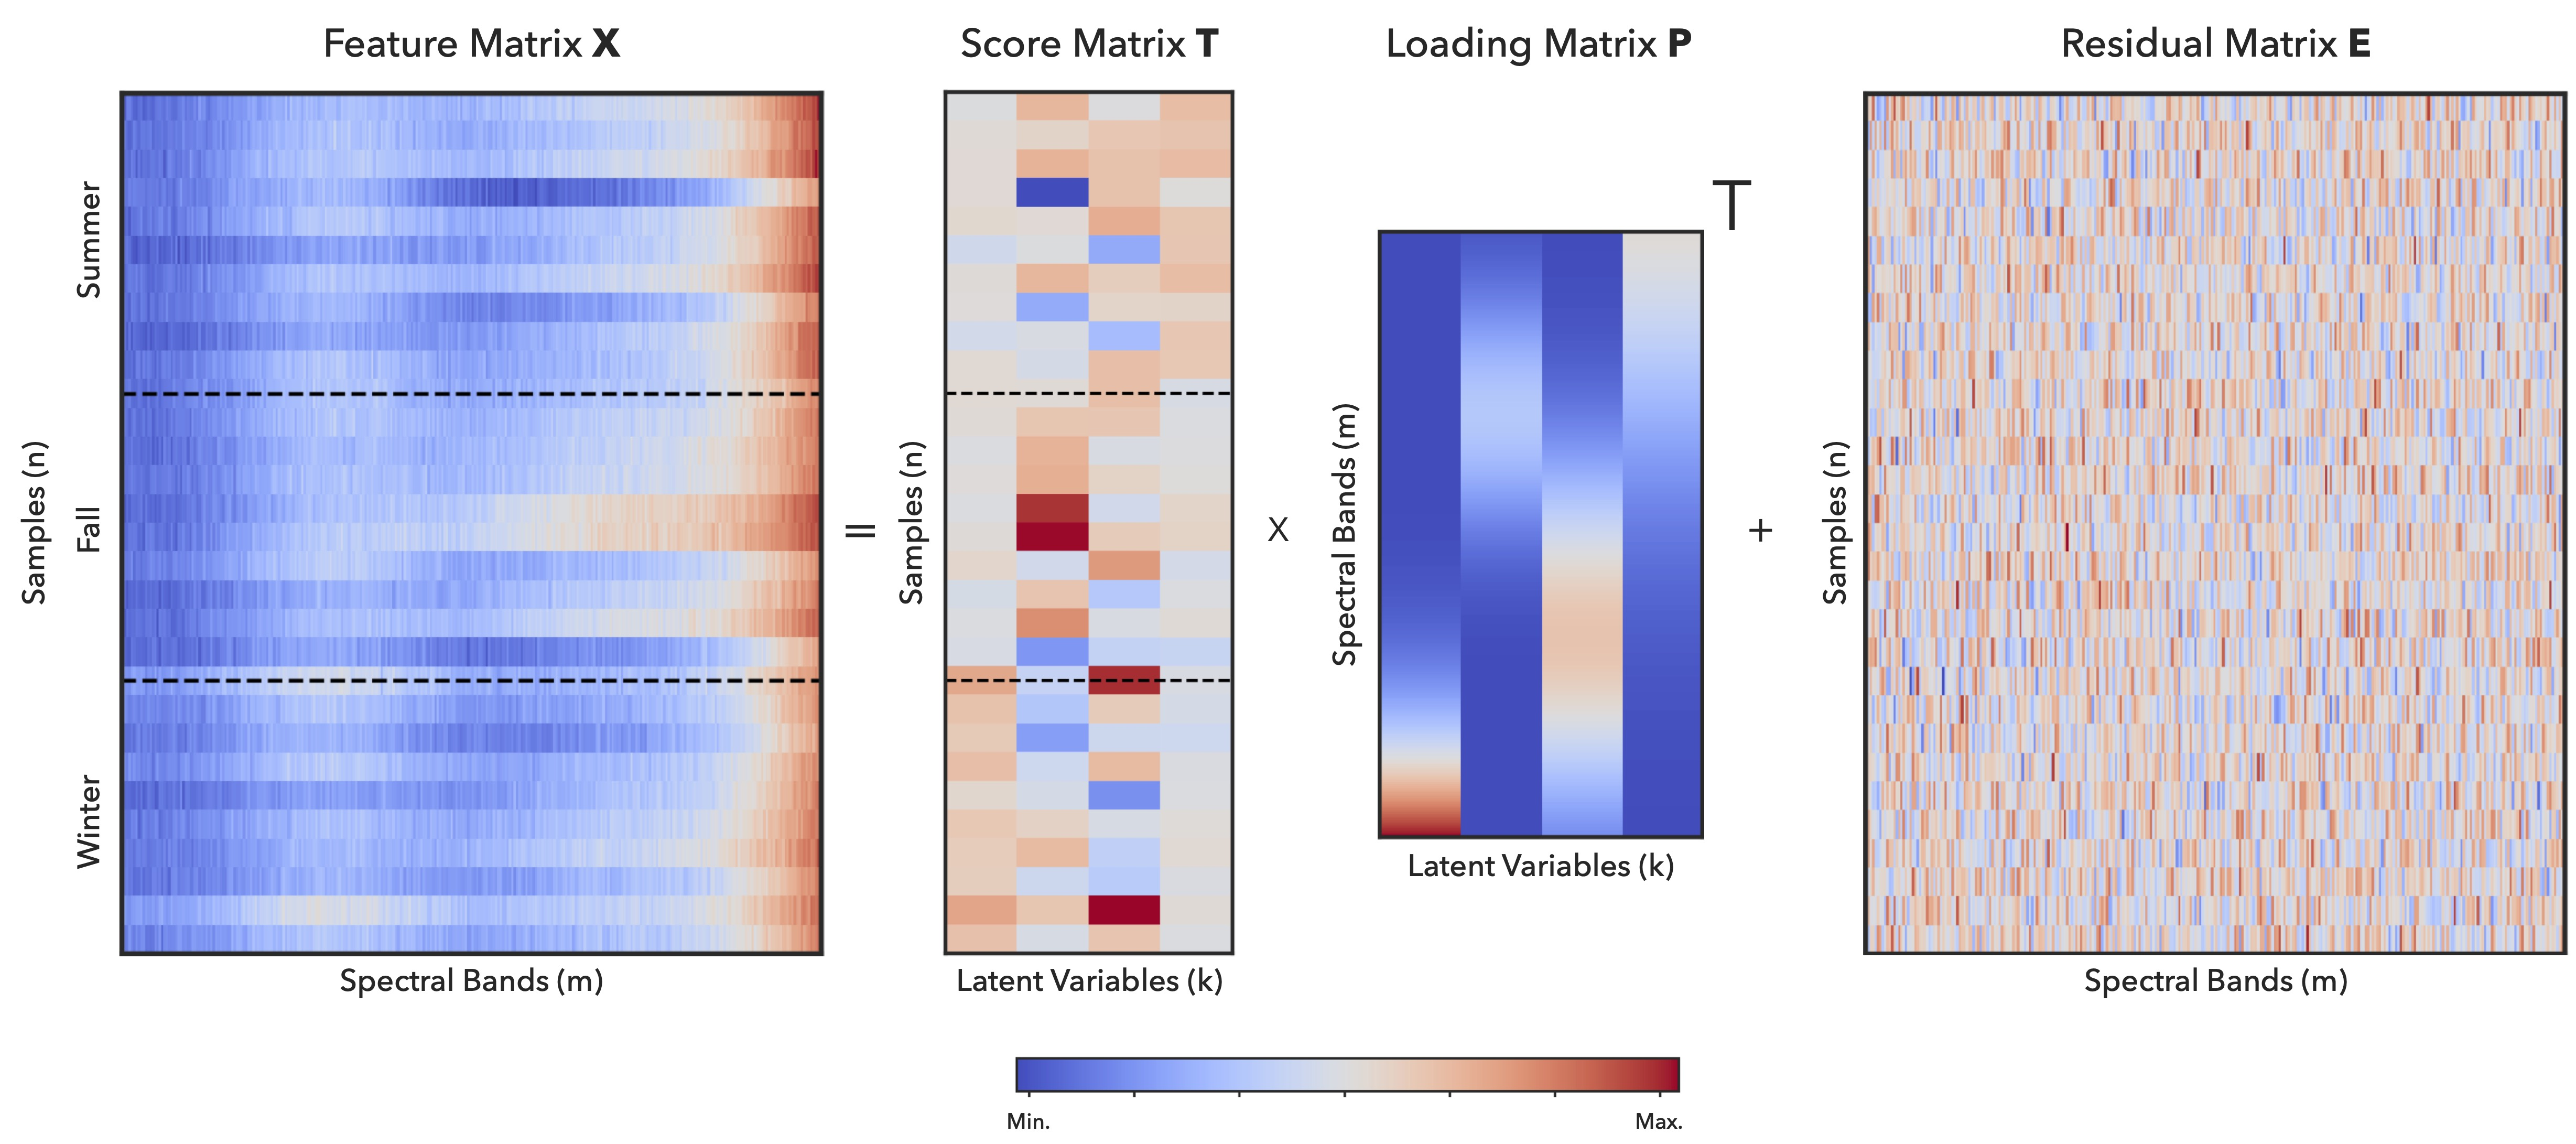
\includegraphics[width=1\textwidth]{fig_1.jpg}
    \caption{Matrix decomposition of the simulated spectral data. The spectral data matrix $X$ is generated as a linear combination of the score matrix $T$ and the loading matrix $P$, with added noise $E$. The color scale is independently normalized for each matrix.}
    \label{fig:1_sim_data}
\end{figure}

The score matrix $T$ defines how each sample contributes to each latent variable. For example, if the third sample exhibits higher spectral measurements around the first peak (as defined by the first latent variable), the value in the third row and first column of the score matrix will be higher relative to other rows. In this study, $T$ was sampled from a multivariate normal distribution with a mean vector of $[1, 1, 1, 1]$ and standard deviations of $[0.02, 0.10, 0.10, 0.02]$. This setup reflects a scenario where the second and third latent variables (corresponding to specific peaks) are more pronounced compared to the first and fourth latent variables. It is inspired by the spectrum measured in the past work \citep{chen_independent_2023}, which used 150 hyperspectral bands ranging from 1,000 nm to 1,600 nm to evaluate the wheat kernel quality trait.

The loading matrix $P$ defines how each spectral variable contributes to each latent variable. Each latent variable in $P$ was simulated using a Gaussian probability function with peaks at the -30$^\text{th}$, 90$^\text{th}$, 200$^\text{th}$, and 345$^\text{th}$ spectral positions and standard deviations of $[100, 40, 60, 60]$ to simulate the width of the peaks. Negative peak positions simulate signals outside the measured spectral range. The residual matrix $E$ is sampled from a normal distribution $\mathcal{N}(0, 0.01)$ to simulate the noise in the spectral data. 

Seasonal variation is an important factor in agricultural studies and is often overlooked in model evaluation. To incorporate this effect, the spectral measurements were simulated across three seasons, with random effects applied to the latent variables. These seasonal effects were modeled by multiplying different scalars with the latent variables in the score matrix $T$. The scalars for the first two latent variables were $[1.00, 1.10, 1.07]$, and for the latter two were $[1.07, 1.00, 1.00]$. This setup reflects a scenario where the first two latent variables are more pronounced in the second and third seasons, while the latter two latent variables dominate in the first season.

The response variable $y$ was generated as a nonlinear function of selected spectral variables. Specifically, four spectral bands ($B$) were selected at indices $[50, 100, 180, 230]$ from the 300 spectral bands. Nonlinear effects were introduced by applying a sinusoidal transformation to the selected spectral variables, raised to the power of three (cubic nonlinearity). To ensure that each effect has a unique sinusoidal component, a phase shift was added to each effect. The phase shift is defined as $\frac{i \pi}{m}$, where $i$ is the index of the selected spectral band, and $m$ is the total number of selected spectral bands. This approach introduces variation in the sinusoidal behavior of each effect, ensuring they are distinct:

$$
y = \sum_{i=1}^{m}\sin(b^3_i + \frac{i \pi}{m}), \quad b_i \in B
$$

where $b_i$ represents the $i$-th selected spectral band from the four bands $B$. Finally, Gaussian noise was added to the response variable $y$ to simulate measurement or modeling errors. The noise was generated with a standard deviation equal to that of the response variable $y$, simulating a scenario where only 50\% of the variance in $y$ can be explained by the spectral data. This approach introduces realistic variability, reflecting the inherent uncertainties and complexities often encountered in real-world prediction tasks.


\begin{figure}[H]
    \centering
    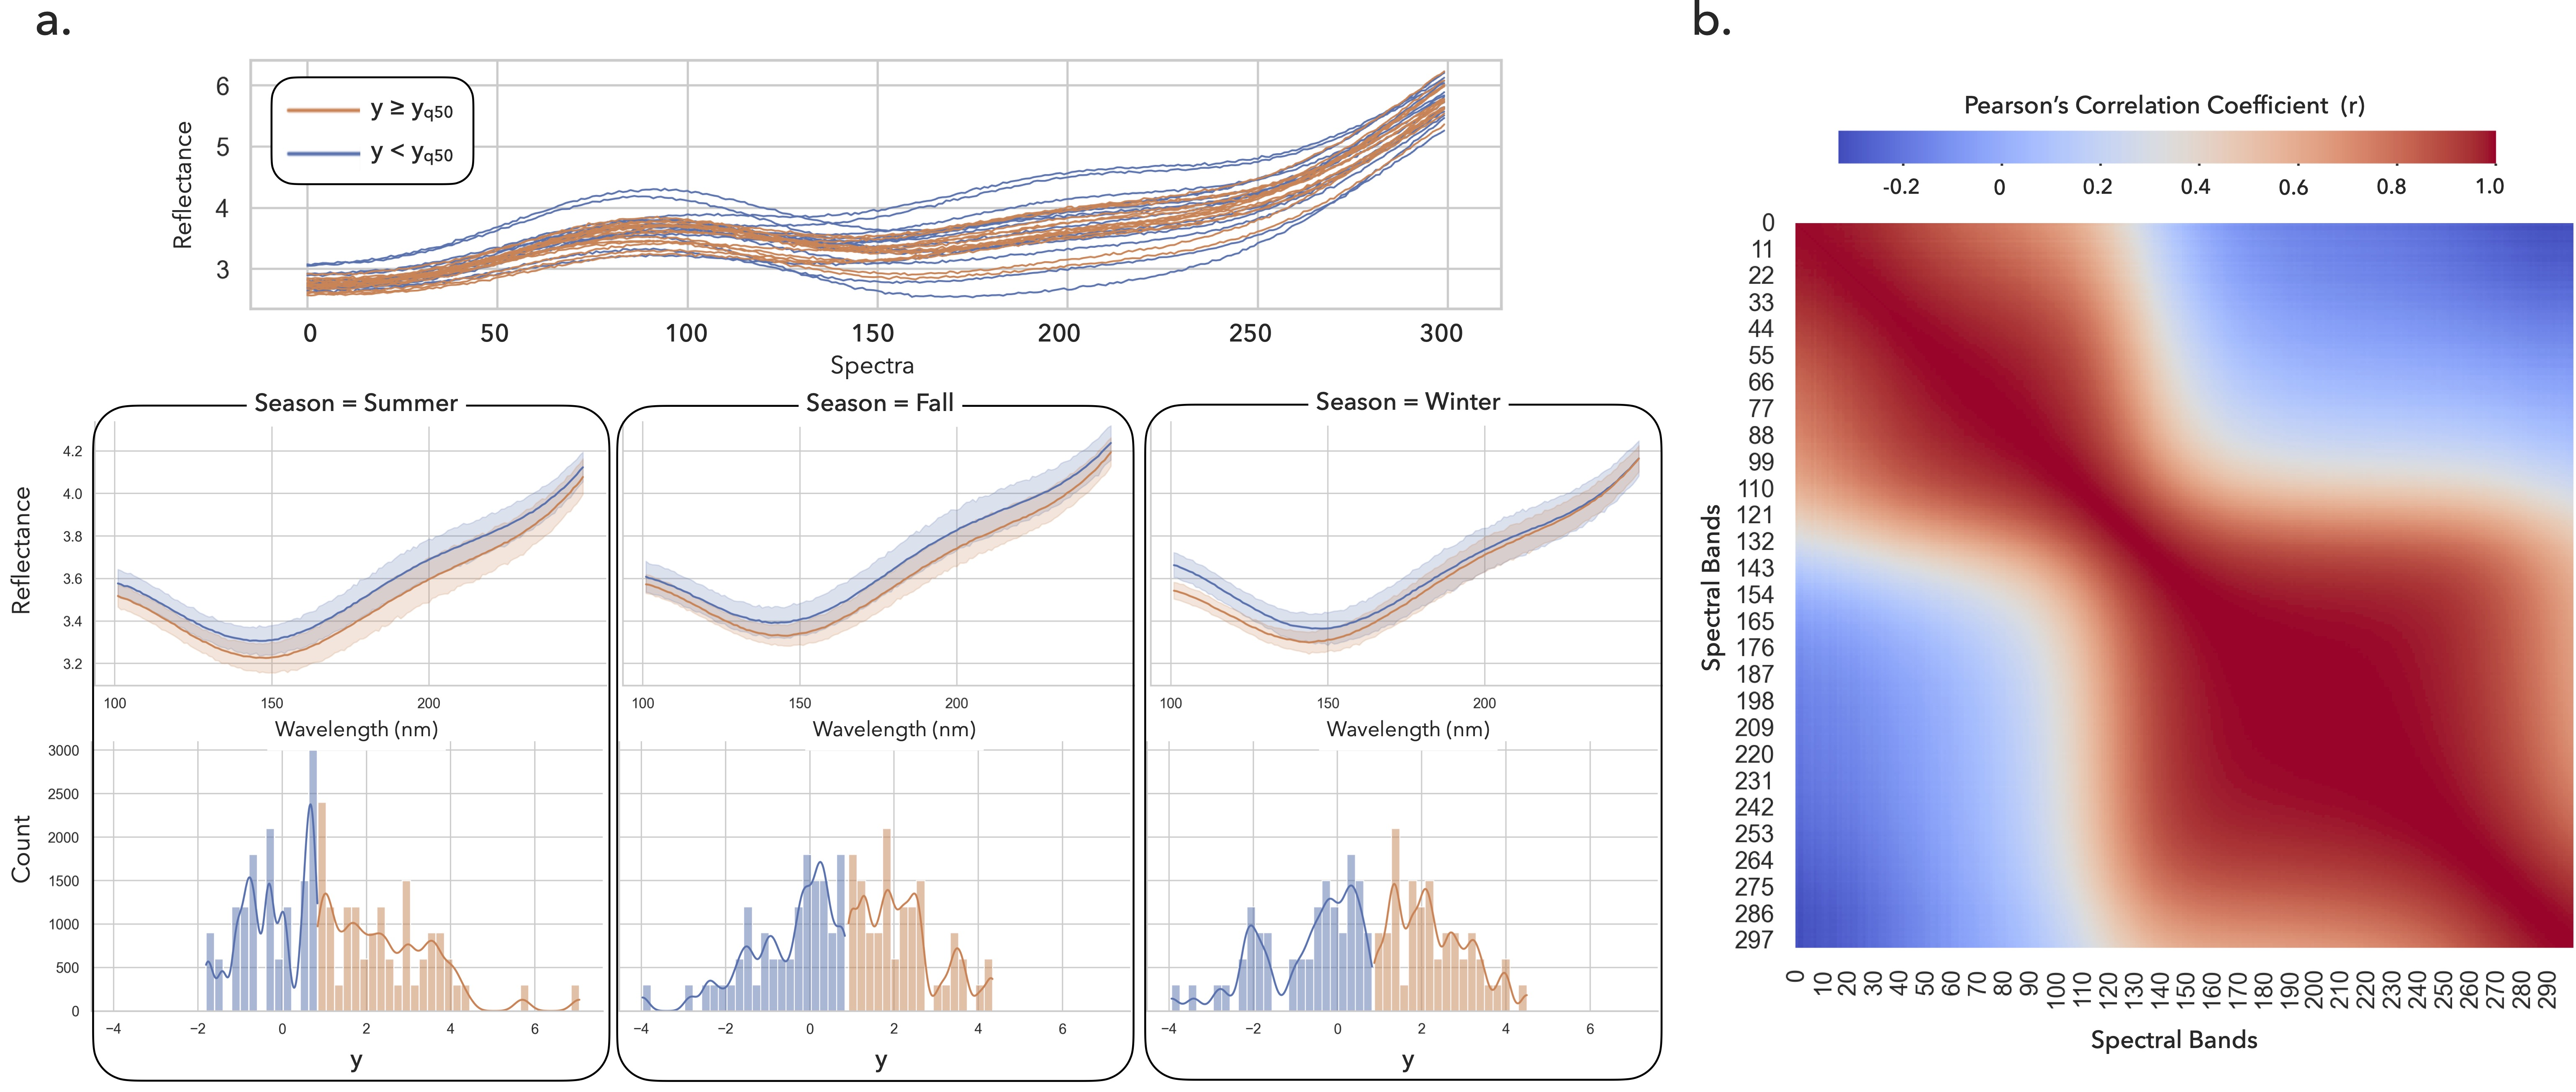
\includegraphics[width=1\textwidth]{fig_2.jpg}
    \caption{Overview of the simulated spectral dataset. (a) The spectral data matrix $X$ is visualized with the target variable $y$ categorized by its median value. (b) The autocorrelation plot of the spectral data matrix $X$ shows a bi-modular correlation structure.}
    \label{fig:2_sim_data}
\end{figure}

The simulated spectral data exhibit a bi-modular autocorrelation structure, with the least pair-wise correlation (r=0.4) observed near the 100th band, which serves as the cutoff between the two modules (Figure ~\ref{fig:2_sim_data}b). The non-linear relationship between the spectral data and the target variable $y$ is evident when $y$ is categorized by its median value ($y_{\text{q}50}$) and visualized in two color groups within the spectral space (Figure ~\ref{fig:2_sim_data}a). The resulting plot reveals that the data are not linearly separable in the spectral space, confirming the expected complexity and presenting a challenging task for model evaluation. Additionally, seasonal effects simultaneously influence both the spectral data and the target variable. For instance, the spectral reflection is less pronounced around the 150th band during the first season, while the separability of the two categorical groups decreases around the 250th band in the third season. Furthermore, the distribution of the target variable varies across seasons: the first season displays a right-skewed distribution, whereas the other two seasons have more symmetric distributions. These seasonal variations introduce additional layers of complexity, further highlighting the importance of robust evaluation methods for classification models.

\subsubsection{Real-world spectral dataset}

This dataset contains spectral data collected across 18 bands ranging from 410 nm to 940 nm, aimed at assessing forage quality. The spectral data were captured using a SparkFun ESP32 Thing Plus microprocessor paired with a SparkFun Triad Spectroscopy Sensor (SparkFun Electronics, Niwot, CO). The sensor suite was programmed using Arduino IDE v2.0.4 (Arduino Core Team, 2024) to export measurements.

Forage quality was quantified based on neutral detergent fiber (NDF) content, a critical parameter for evaluating livestock nutrition. Ground truth NDF values were determined using traditional bench chemistry methods with the ANKOM 200 fiber analyzer system (ANKOM Technology, Macedon, NY). The dataset comprises 599 samples collected over three distinct time periods reflecting the seasonal effects on both the spectral data and the NDF response: 189 samples were collected from May to June, 198 from July to August, and 212 from September to October. Sampling took place weekly between May 1 and October 30, 2023, with two samples collected each week from each of 12 fields. Within each field, sampling locations were chosen at random and varied from week to week.

The spectral data were collected in the field using a handheld sensor, while NDF content was measured in the lab. The fields were primarily grazed by cattle, with some fields grazed by other species, including sheep and horses. This dataset provides a comprehensive view of how seasonal variation influences forage quality and spectral characteristics, offering valuable insights into the dynamics of pasture composition and livestock nutrition.

\begin{figure}[H]
    \centering
    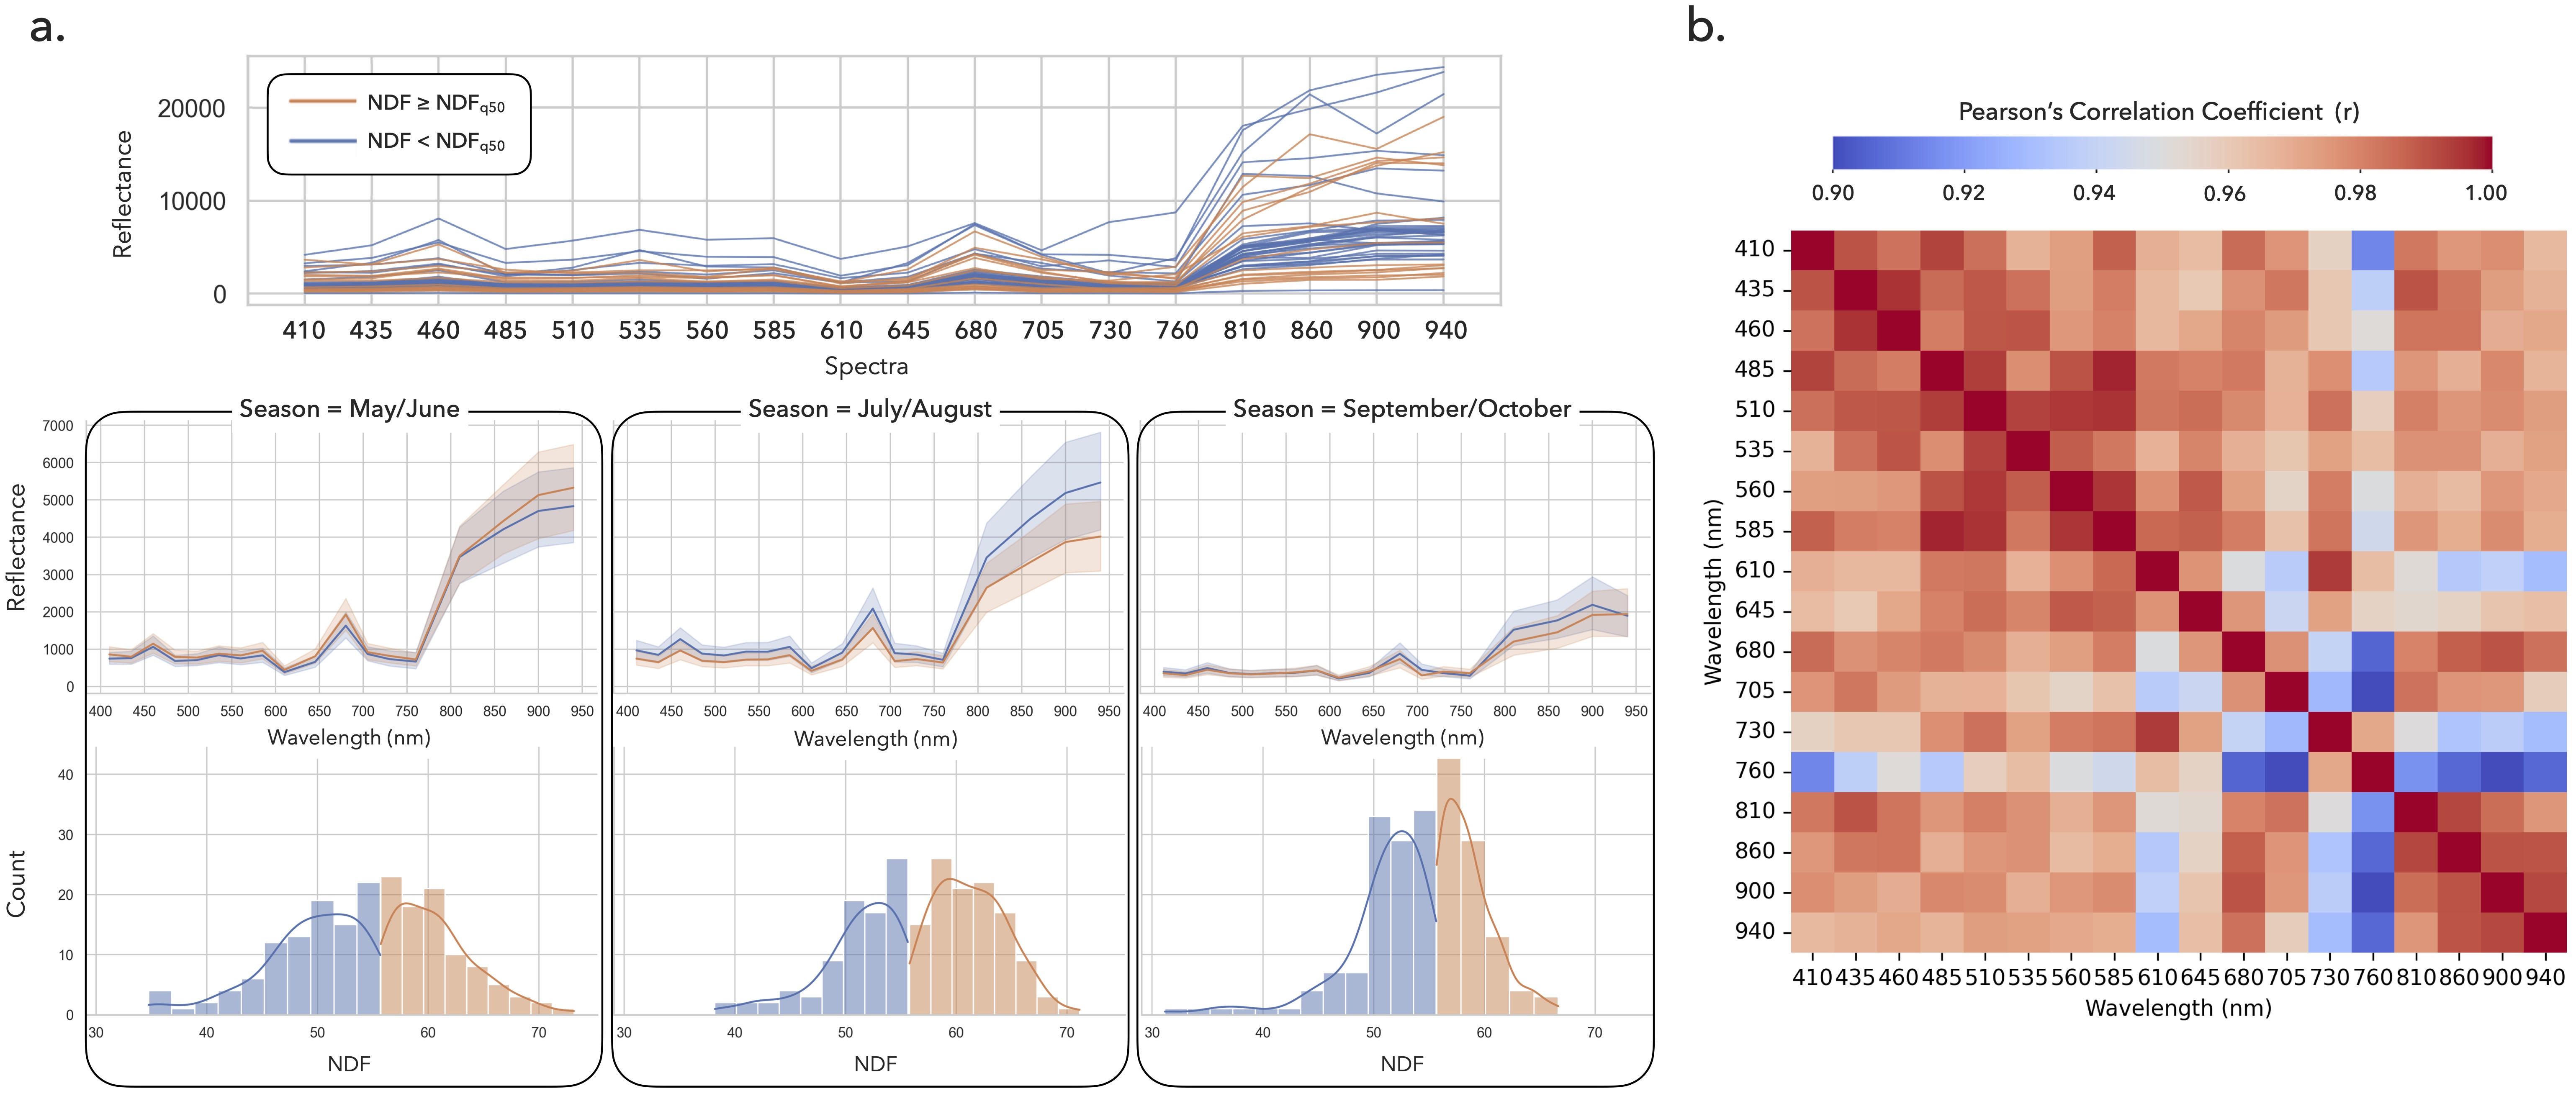
\includegraphics[width=1\textwidth]{fig_3.jpg}
    \caption{Overview of the real spectral dataset. (a) The spectral data matrix $X$ is visualized with the neutral detergent fiber (NDF) $y$ categorized by its median value. (b) The autocorrelation plot of the spectral data matrix $X$.}
    \label{fig:3_real_data}
\end{figure}

A similar examination of the data structure was conducted for both the spectral measurements and the target variable (Figure ~\ref{fig:3_real_data}). The autocorrelation in the spectral measurements is notably stronger than in the simulated dataset, with at least 0.90 for pairwise Pearson correlation coefficients. The seasonal interactions among the spectral measurements are also more pronounced compared to the simulated data. For instance, the spectral reflectance measured in September and October is roughly halved compared to the other seasons. Additionally, a distinct seasonal pattern was observed in the reflectance data beyond 800 nm. In July and August, samples with lower NDF value tend to exhibit higher spectral reflectance, whereas this trend is not evident in May–June or September–October. Moreover, the NDF distribution shows greater variability in July and August, with a higher standard deviation (7.15) compared to May–June (6.19) and September–October (5.23). These observations highlight the stronger seasonal effects and variability in the real dataset compared to the simulated data, providing another example of the challenges in evaluating model performance in real-world agricultural studies.
\subsection{Experiment 1: Evaluation bias and variance of cross-validation}

This experiment examined the reliability of CV in estimating model performance, with a focus on different performance estimators and their interaction with sample size. It is hypothesized that increasing the number of folds in CV will generally provide a more accurate estimate of model performance but will also lead to increased variance in each estimate, as suggested by the bias-variance trade-off theory. Additionally, sample size is considered a critical factor in reducing the bias difference between estimators, with larger sample sizes expected to mitigate the impact of estimator bias and improve the reliability of performance evaluation.

Since K-fold CV employs a fraction (i.e., $K-1$ folds) of the data for training, it may provide a pessimistic estimate of model performance. 
Such underestimation is explored in this experiment by comparing the performance metrics of K-fold CV with K set to 2, 5, and 10, as well as LOOCV where K equals the sample size N, and the "In-Sample" evaluation, which assesses model performance on the same dataset used for training, potentially leading to an overly optimistic bias. To gauge model performance, four metrics are employed: RMSE (Eq. ~\ref{eq_rmse}), MAE (Eq. ~\ref{eq_mae}), r (Eq. ~\ref{eq_r}), and $R^2$ (Eq. ~\ref{eq_R2}). The evaluation model is a linear regression with ten input features and one output target, all drawn from the null dataset. The sample sizes N are varied among 50, 250, and 500 to explore the dynamics between sample size and performance estimators. Each configuration is repeated across 500 iterations to assess the distribution of evaluation bias and variance.

For each iteration, the dataset $\mathcal{D}={(X, y)}$ was sampled as per the simulation’s premise. In the case of K-fold CV, the dataset $\mathcal{D}$ was partitioned into K folds in which each fold is $\mathcal{D}_k={(X_k, y_k)}$. For the “In-Sample” approach, partitioning does not occur. The linear model $f$ is trained on the training set $\mathcal{D}_\text{-k}$ (denoted as $f_{\mathcal{D}_{\text{-k}}}$) to estimate regression coefficients $\beta$, which then predicts the target variable ${\hat{y}}_k$ from the test set $\mathcal{D}_k$. The procedure of K-fold CV can be expressed as:

\begin{equation} \label{eq_kfoldcv}
    \begin{split}
	\text{Training: } \quad y_{\text{-k}} &= f_{\mathcal{D}_{\text{-k}}}(X_{\text{-k}})+\epsilon \\
    &= X_{\text{-k}} \beta + \epsilon \\
    \text{Testing: } \quad \hat{y}_k &= f_{\mathcal{D}_{\text{-k}}}(X_k) \\
    &=X_k \beta \quad \quad \quad k=1,2,\ldots,K
    \end{split}
\end{equation}

For the “In-Sample” performance estimator, predictions were made without splitting, as:

\begin{equation} \label{eq_insample}
    \begin{split}
    	\text{Training: } \quad y &= f_\mathcal{D}(X) \\ &= X\beta + \epsilon \\
        \text{Testing: } \quad \hat{y} &= f_\mathcal{D}(X) \\ &=X \beta
    \end{split}
\end{equation}

Where:
\begin{itemize}
  \item \( X \) denotes the input regressors sampled from a standard normal distribution \( \mathcal{N}(0, 1) \) with dimensions \( N \times 10 \).
  \item \( y \) denotes the target variable sampled from a standard normal distribution \( \mathcal{N}(0, 1) \) with dimensions \( N \times 1 \).
  \item \( X_\text{-k} \) and \( y_\text{-k} \) are the input regressors and target variable in the training set \( \mathcal{D}_\text{-k} \).
  \item \( X_k \) denotes the input regressors in the test set \( \mathcal{D}_k \).
  \item \( \hat{y}_k \) denotes the predicted target variable in the test set \( \mathcal{D}_k \).
  \item \( \beta \) denotes the estimated regression coefficient with dimensions \( 10 \times 1 \).
  \item \( \epsilon \) denotes the error term assumed to be normally distributed.
\end{itemize}

Estimated performance $\mathbb{E}[\hat{g}(f_\mathcal{D})]$ was derived by averaging the performance metrics across all K folds as per Eq. ~\ref{eq_g_exp}. The bias and variance of the evaluation were calculated using Eqs. ~\ref{eq_bias} and ~\ref{eq_var}, respectively. To approximate true model performance $G(f_\mathcal{D})$, a hundred unseen datasets $\mathcal{D}^\ast$ were generated identically to $\mathcal{D}$, and the performance $G(f_\mathcal{D})$ was estimated by averaging the performance metrics across all $\mathcal{D}^\ast$. The detailed steps to compute evaluation bias and variance are provided in the supplementary materials.

\subsection{Experiment 2: Model Selection in Cross-Validation}

The objective of this simulation experiment is to investigate the impact of improper model selection practices on evaluation bias. Two critical steps in the model selection process are considered: feature selection and hyperparameter tuning. The experiment hypothesizes that improper model selection — particularly the leakage of test set information during feature selection or hyperparameter tuning — will result in a significant overestimation of model performance.

To evaluate this hypothesis, three datasets are utilized: a null dataset with a baseline performance of  $r = 0$, a simulated spectral dataset, and a real spectral dataset. Feature selection is conducted by selecting the top 10 features most strongly correlated with the target variable, $y$. The original number of feature candidates varies across datasets, with 1000 for the null dataset, 300 for the simulated spectral dataset, and 18 for the real spectral dataset.

For hyperparameter tuning, the experiment employs a Support Vector Regression (SVR) model with two hyperparameters: the kernel function and the regularization parameter ($c$). The kernel functions considered are linear, sigmoid, and radial basis function (RBF), while the regularization parameter is set to two values: $c = 1.0$  and  $c = 0.01$. The kernel function determines how the selected features are transformed — either linearly or nonlinearly — to predict the target variable, $y$. The regularization parameter $c$ controls the trade-off between minimizing prediction error and model complexity; a larger $c$ allows for more error but reduces the likelihood of overfitting. In total, six SVR model variants (i.e., three kernel functions combined with two regularization parameter values) are available for selection during the evaluation process.

\begin{figure}[H]
    \centering
    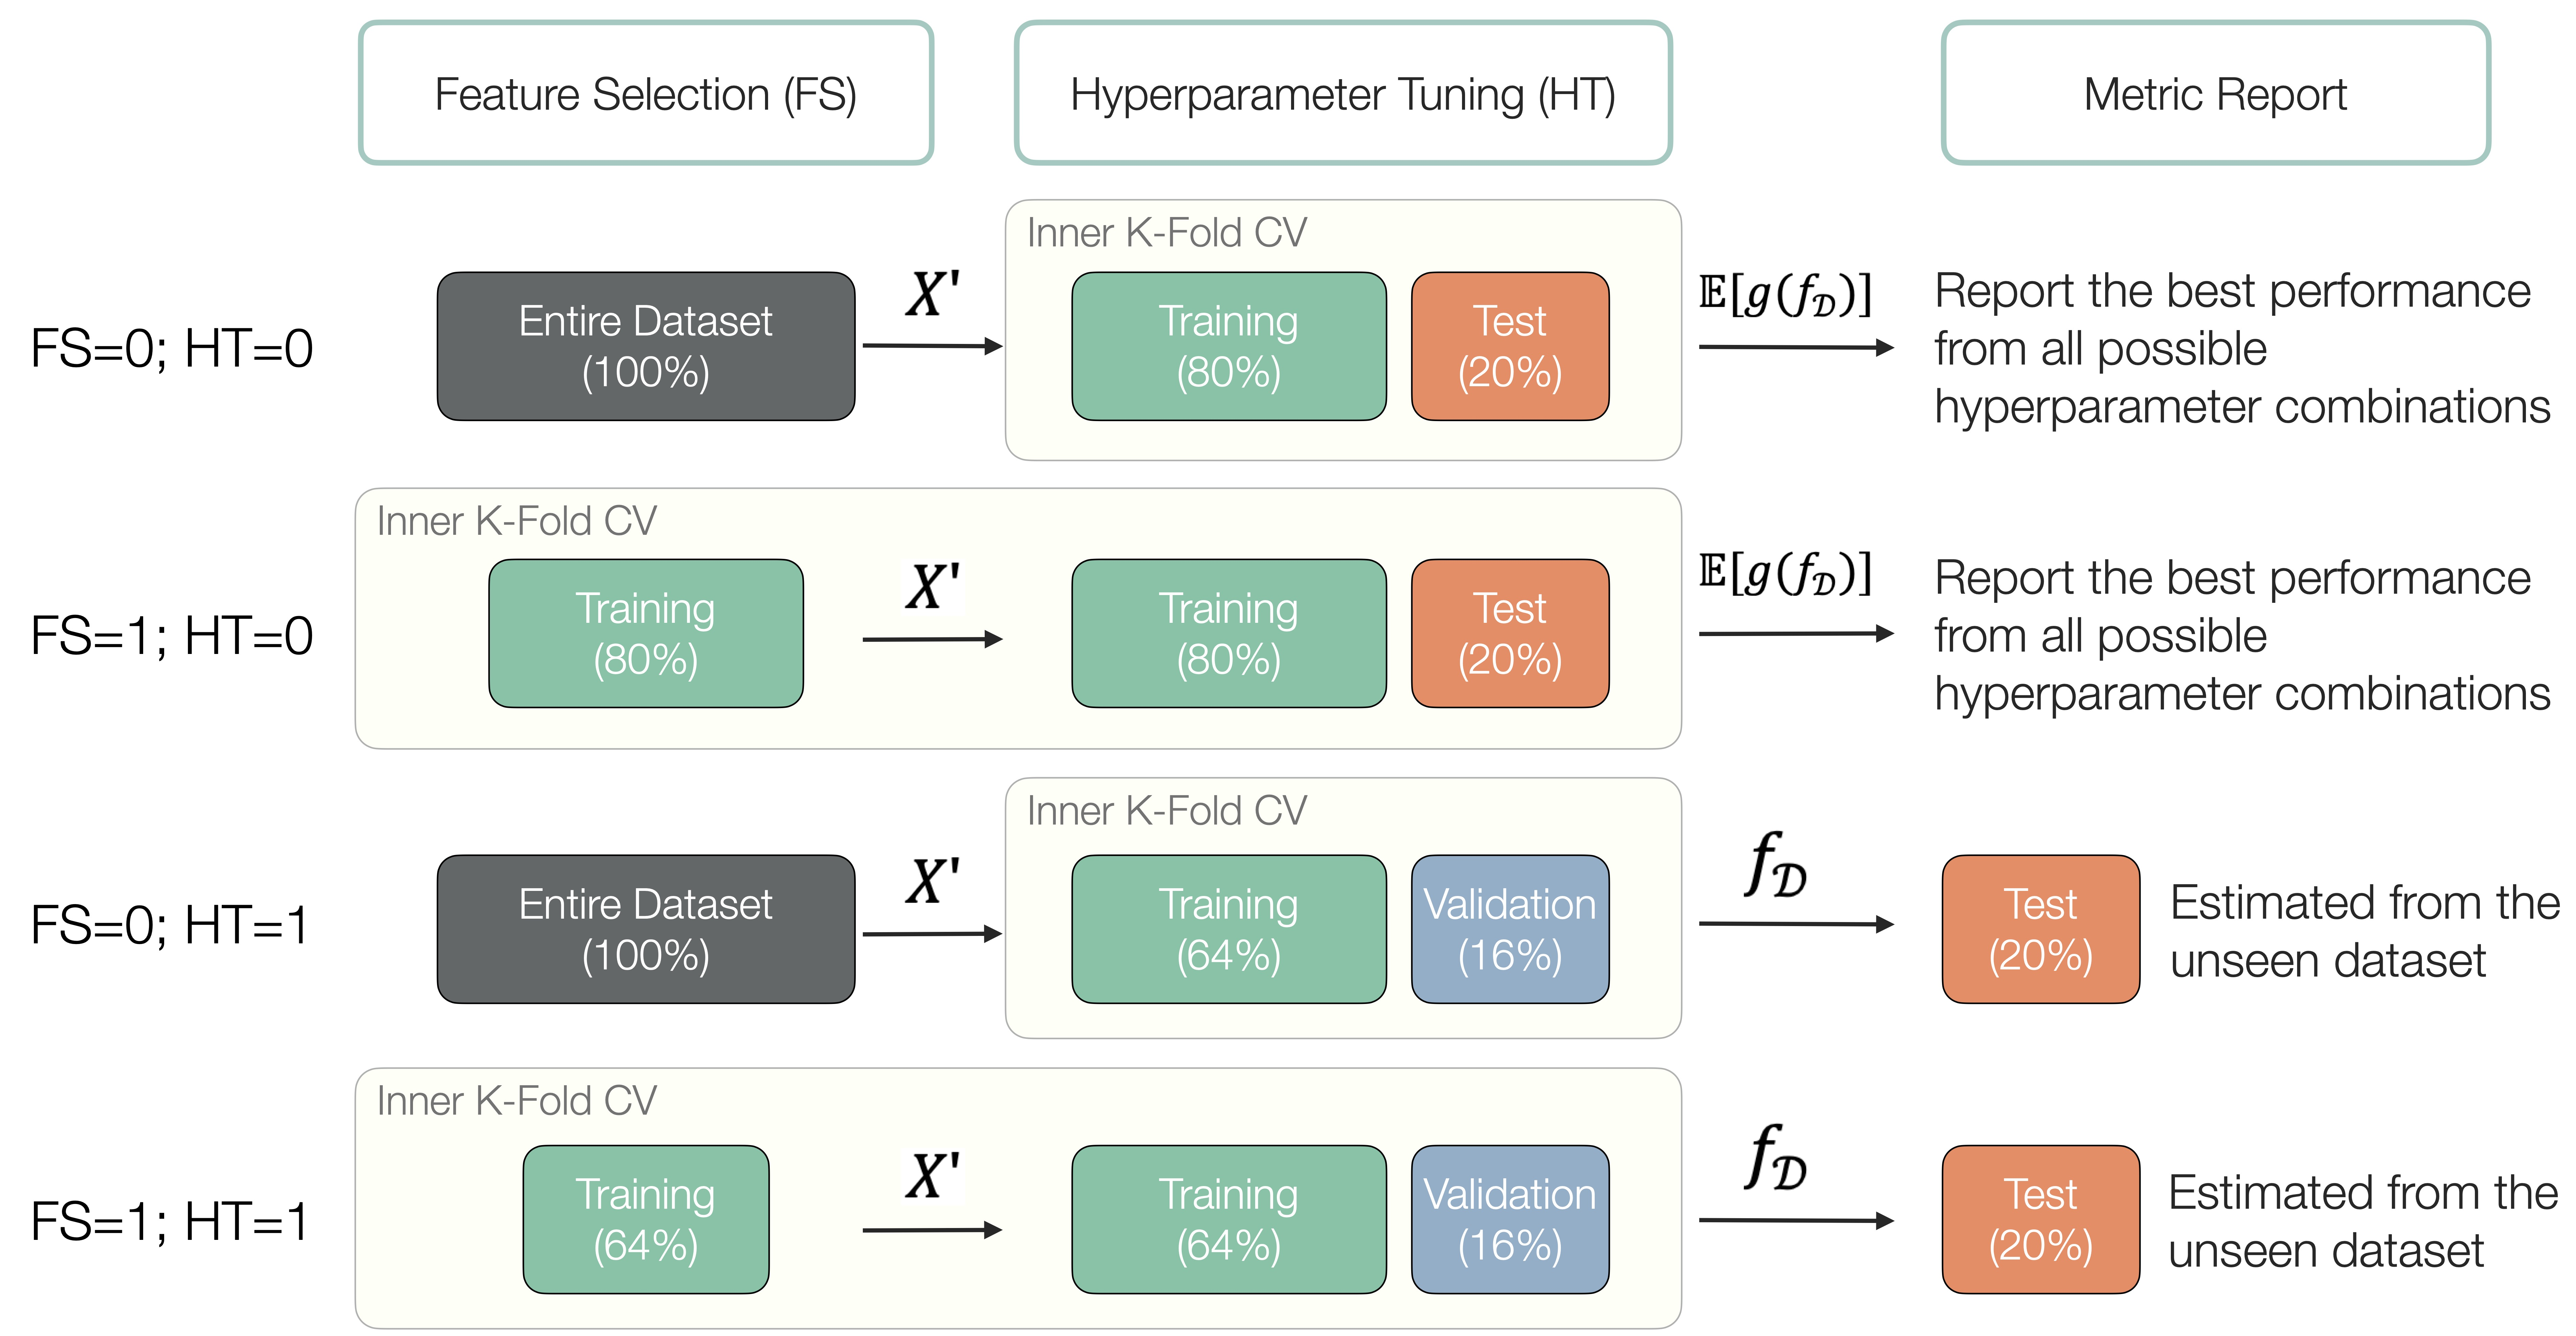
\includegraphics[width=1\textwidth]{fig_s2_schemes.jpg}
    \caption{Workflow diagram illustrating four cross-validation strategies of feature selection (FS) and hyperparameter tuning (HT), where 0 denotes incorrect implementation and 1 indicates correct practice. $X'$ is the selected feature subset, $\mathbb{E}[\hat{g}(f_\mathcal{D})]$ is the expected generalization performance, $f_\mathcal{D}$ is the model trained on the training set without being revealed to the test set.}
    \label{fig:s2_schemes}
\end{figure}

This experiment introduces notations FS for feature selection and HT for hyperparameter tuning, assigning a binary indicator (0 or 1) to denote incorrect (0) or correct (1) implementation of model selection. This yields four possible combinations of model selection strategies: “FS=0; HT=0”, “FS=0; HT=1”, “FS=1; HT=0”, “FS=1; HT=1” (Figure ~\ref{fig:s2_schemes}). When FS=0, feature selection precedes cross-validation splitting. If FS=1, feature selection occurs within each fold of the training set during cross-validation. With hyperparameter tuning, a correct implementation (HT=1) involves splitting the dataset into training (64\%), validation (16\%), and test (20\%) sets. The model is trained and tuned using the training and validation sets, respectively, while the test set is reserved for a single evaluation of model performance. Conversely, with HT=0, only training (80\%) and test (20\%) sets are used, risking evaluation bias as the test set informs both training and performance reporting. A 5-fold cross-validation approach was deployed for all strategies.
evaluation bias is measured as the discrepancy between the model selection-influenced performance estimate and the expected generalization performance (r=0), using the Pearson correlation coefficient between predicted and observed values. Over 500 sampling iterations, the experiment assesses the distribution of evaluation bias. A two-way analysis of variance (ANOVA) was conducted to examine the main effects of HT and FS on model performance. The ANOVA model was specified as $y \sim 1 + \text{HT} + \text{FS}$. This experimental setup is designed to quantify the extent of performance overestimation under improper model selection practices and provide insights into its implications for predictive modeling.
\subsection{Experiment 3: Block Effects in Cross-Validation}

\begin{figure}[H]
    \centering
    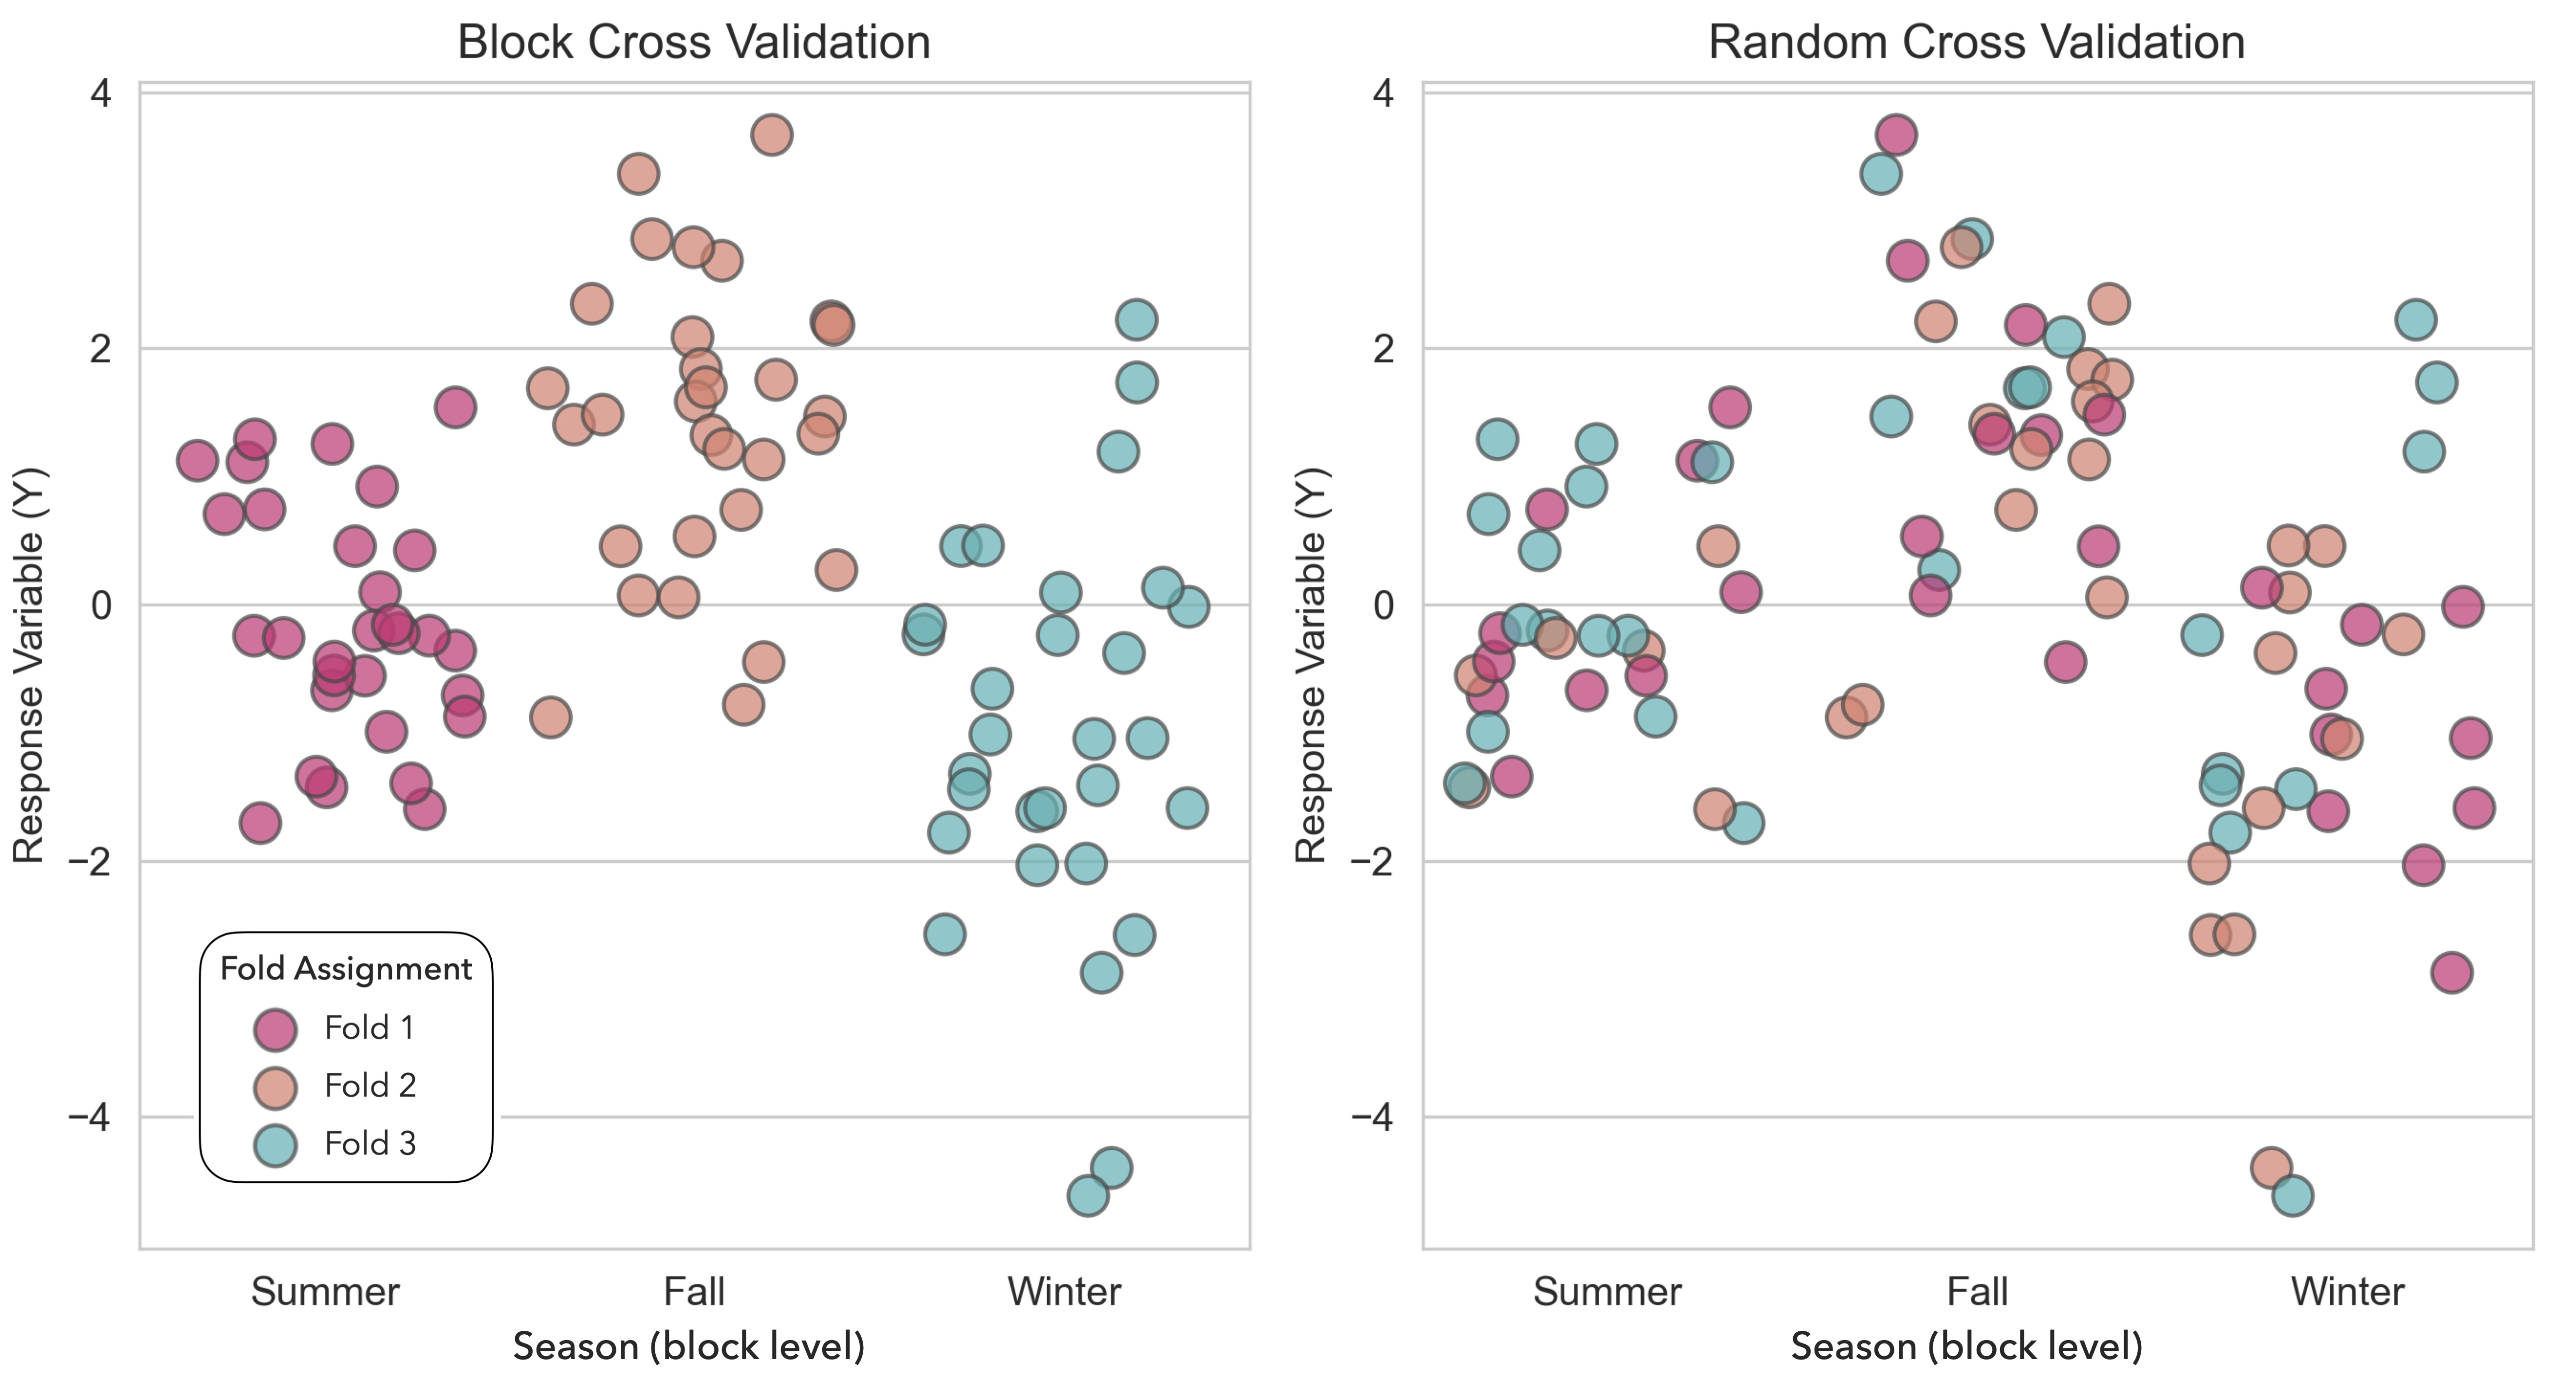
\includegraphics[width=.8\textwidth]{fig_s3_block.jpg}
    \caption{Illustration of fold assignment in block cross validation (left) and random cross validation (right). Folds are color-coded, and the block effect is set to 3 in this example.}
    \label{fig:s3_block}
\end{figure}

The objective of this experiment is to demonstrate how Random CV, which randomly assigns samples to folds without accounting for block effects, can lead to an overestimation of model performance. As a benchmark, the experiment employs Block CV, where each block is treated as a fold in cross-validation. The hypothesis is that the model performance estimated by Random CV will be significantly higher than that estimated by Block CV.

This experiment utilizes both simulated and real-world datasets, both of which were collected across multiple seasons, introducing block effects that confound both the predictor features and the response variable. The simulated dataset includes 200 observations per season, distributed equally across seasons, while the real-world dataset also contains approximately 200 observations per season. The block effect in both datasets is defined by the seasonal variation.

The experiment evaluates two model validation strategies: Block CV and Random CV, both using a 3-fold cross-validation approach. Three folds are used to match the number of seasons in the dataset. In Block CV, each block (i.e., season) is treated as a distinct fold, ensuring that samples from the same block are not split across folds. In Random CV, samples are randomly assigned to folds without consideration of block boundaries (Figure ~\ref{fig:s3_block}). The predictive model used is a random forest regression model, and its performance is assessed using Pearson’s correlation coefficient $r$ and RMSE.

The simulation is run for 500 iterations, with $X$ (predictor variables) and $Y$ (response variable) resampled in each iteration for the simulation dataset and also the fold assignment to account for variability. A one-way ANOVA was performed to evaluate whether the choice of CV strategy (i.e., block CV vs. random CV) significantly affects model bias. The model was specified as $y \sim 1 + \text{BlockCV}$,

\subsection{Experiment 4: Characteristics of Metrics in Regression Tasks}

\begin{figure}[H]
    \centering
    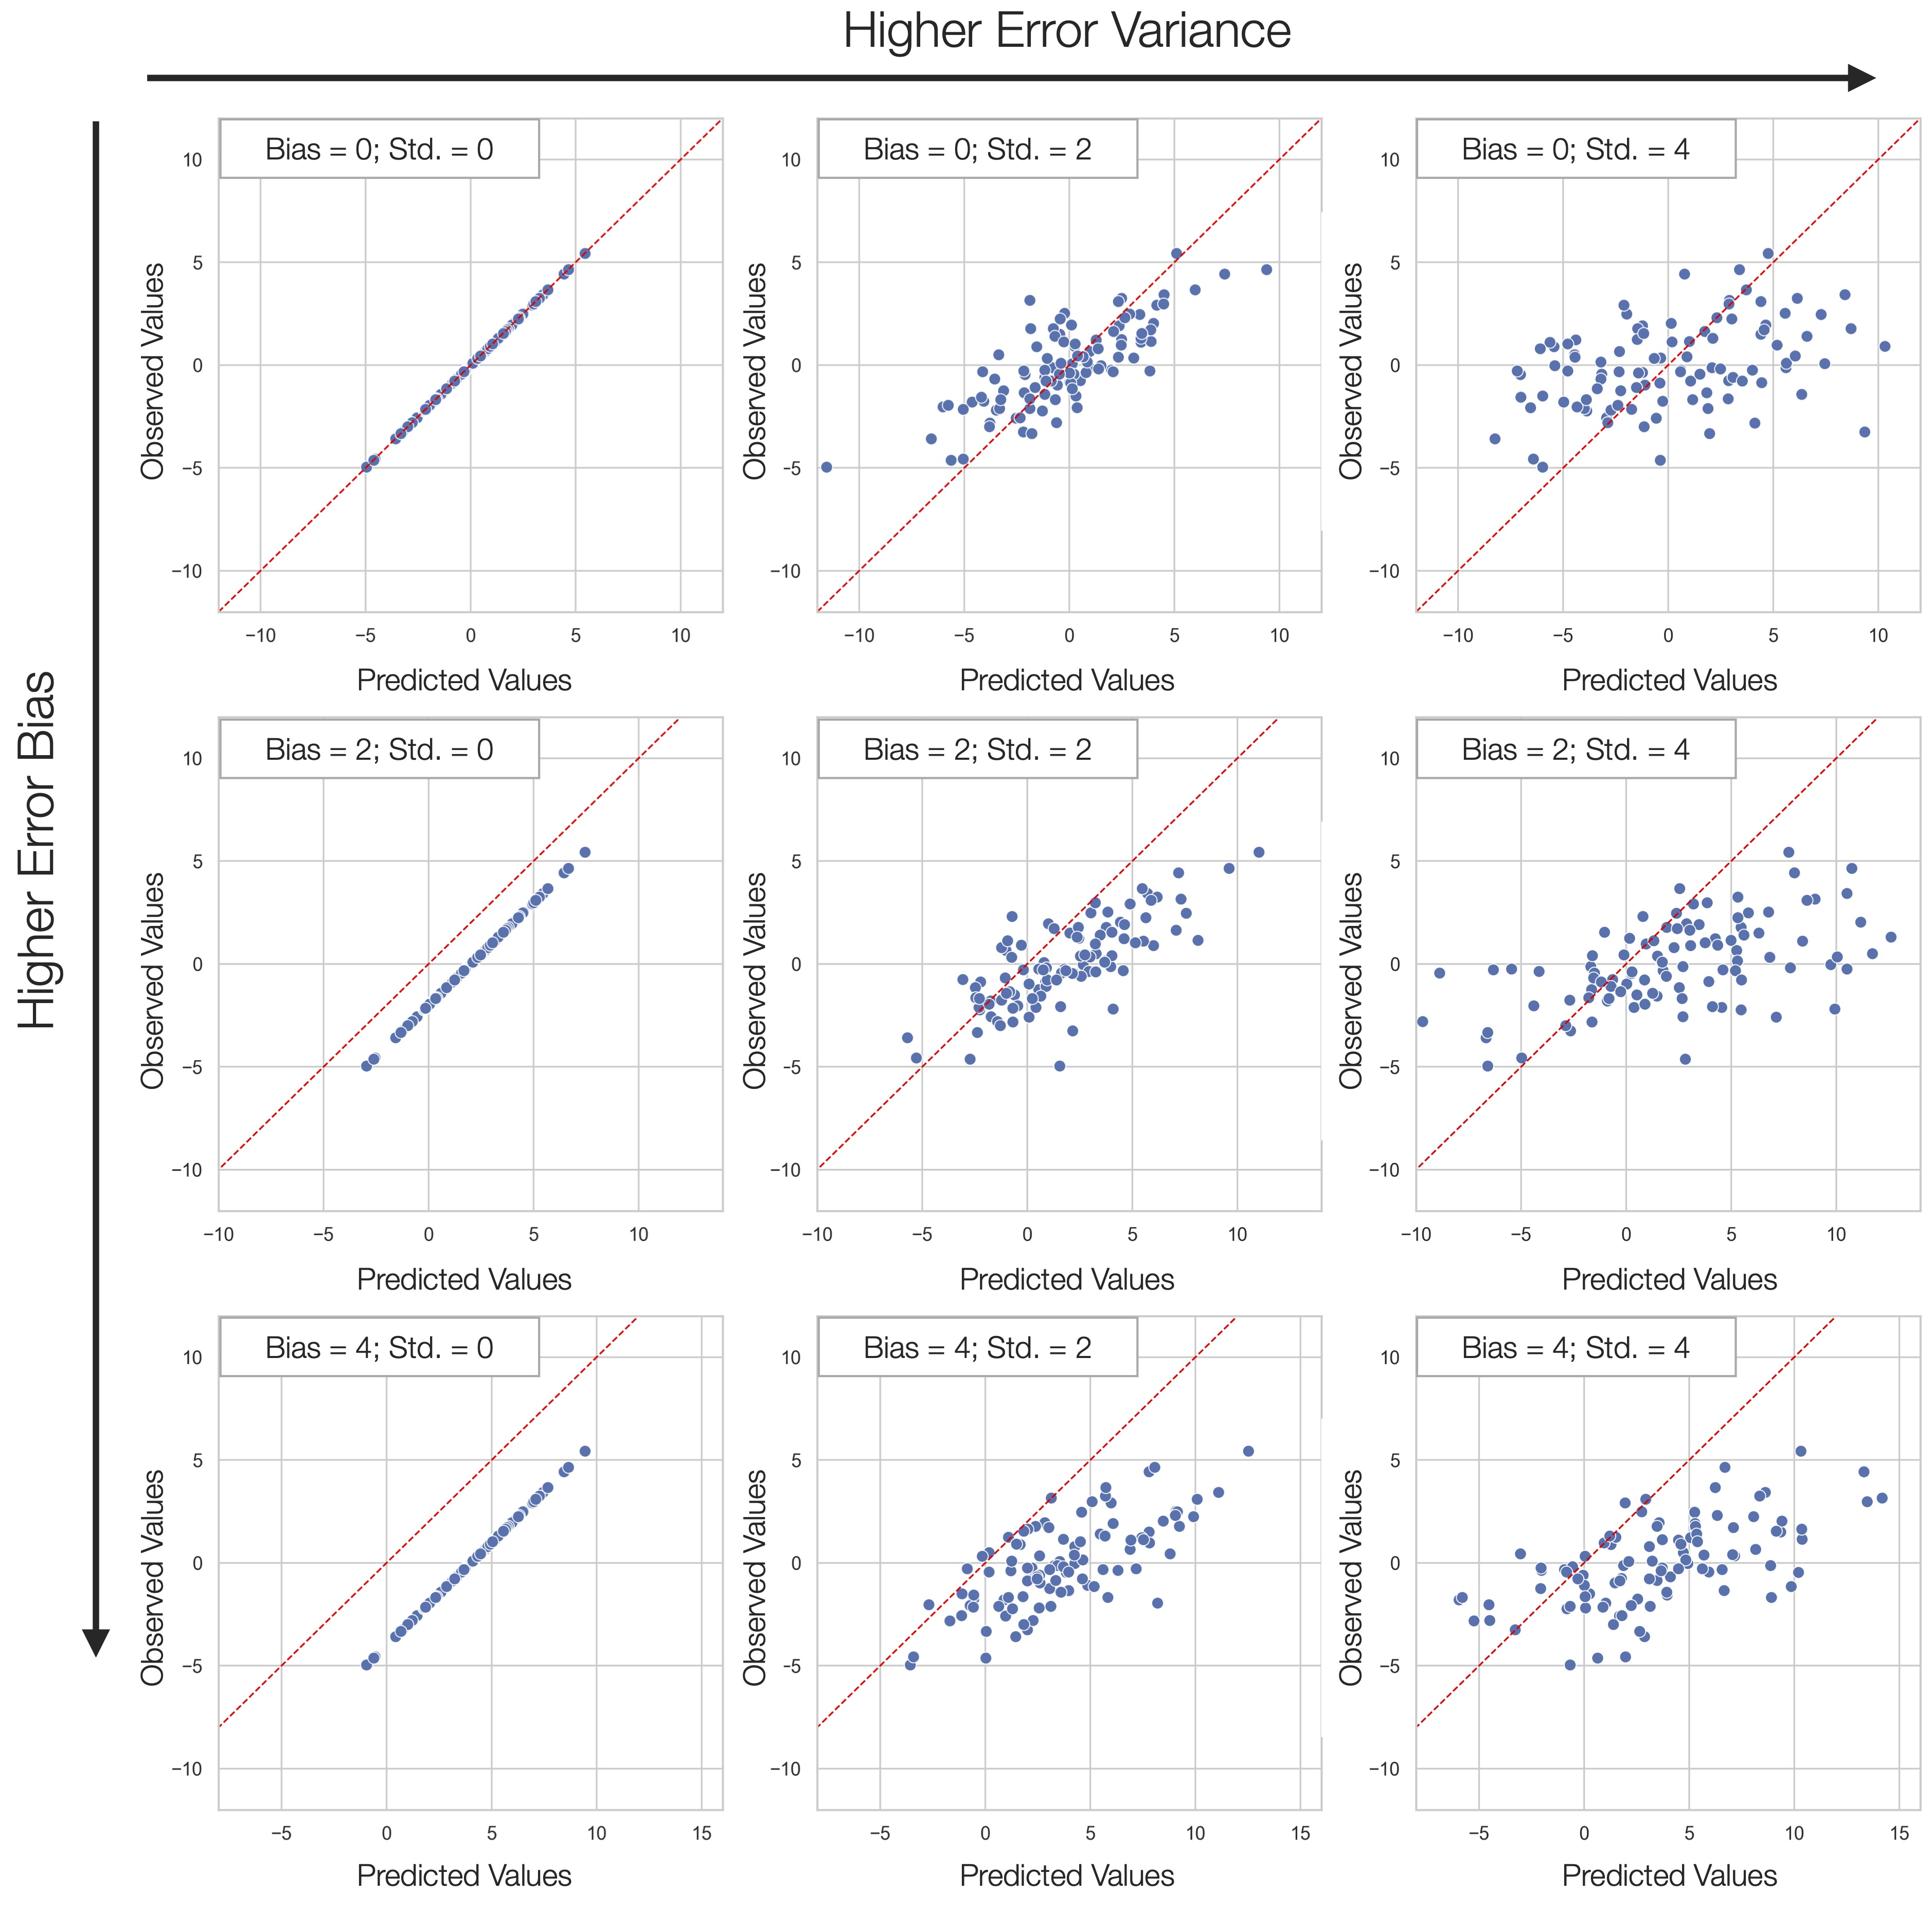
\includegraphics[width=1\textwidth]{fig_4.jpg}
    \caption{Scatter plots illustrating the relationship between predicted and actual values for 9 combinations of bias and variance, with each parameter set to one of three levels: 0, 2, or 4. The red diagonal line represents the ideal prediction line.}
    \label{fig:s4_regression}
\end{figure}

The objective of this experiment is to examine how different performance metrics in regression tasks respond to two types of prediction errors: bias and variance. The experiment aims to highlight the unique characteristics of each metric, such as sensitivity to outliers or systematic bias, and provide guidance for selecting appropriate metrics in regression tasks. Additionally, it seeks to verify the trade-off relationship between bias and variance in prediction errors.

To achieve this, six levels of bias and variance are examined: $[0, 0.5, 1, 2, 4, 8]$, forming a total of 36 combinations of prediction errors. The bias error can be considered as a systematic error that consistently overestimates or underestimates the ground truth values, while the variance error represents the random fluctuations around the ground truth. Outliers of prediction errors are considered as extreme cases of variance errors, where the predicted values deviate considerably from the ground truth. The simulated ground truth values are generated from a normal distribution with a mean of 0 and a standard deviation of 2, while the predicted values ($\hat{y}$) are created by adding random errors ($\epsilon$) with specified levels of bias and variance to the ground truth:

\begin{equation}
\begin{cases}
y \sim \mathcal{N}(0, 2) \\
\epsilon \sim \mathcal{N}(b, s) \\
\hat{y} = y + \epsilon
\end{cases}
\end{equation}

where $b$ represents the bias and $s$ represents the variance of the prediction errors (Figure ~\ref{fig:s4_regression}). The choice of a standard deviation of 2 for the ground truth values is intended to highlight the differences in behavior between the RMSE and RSR metrics, with RSR being standardized by the standard deviation of the ground truth values while RMSE tracks the original error scale.


The evaluated metrics in this experiment are categorized into two main groups. Error-based metrics include RMSE, MAE, and RSR. These metrics focus on quantifying the magnitude of errors in the predictions. Linearity-based metrics, such as $r$, $R^2$, and CCC, assess the linear relationship and agreement between the predicted and actual values. By systematically exploring how each metric responds to varying levels of bias and variance, this experiment demonstrates their strengths, limitations, and practical implications for regression analysis. The findings are intended to guide practitioners in selecting the most appropriate performance metrics based on their specific modeling objectives and the characteristics of their data.


\subsection{Experiment 5: Characteristics of Metrics in Classification Tasks}

\begin{figure}[H]
    \centering
    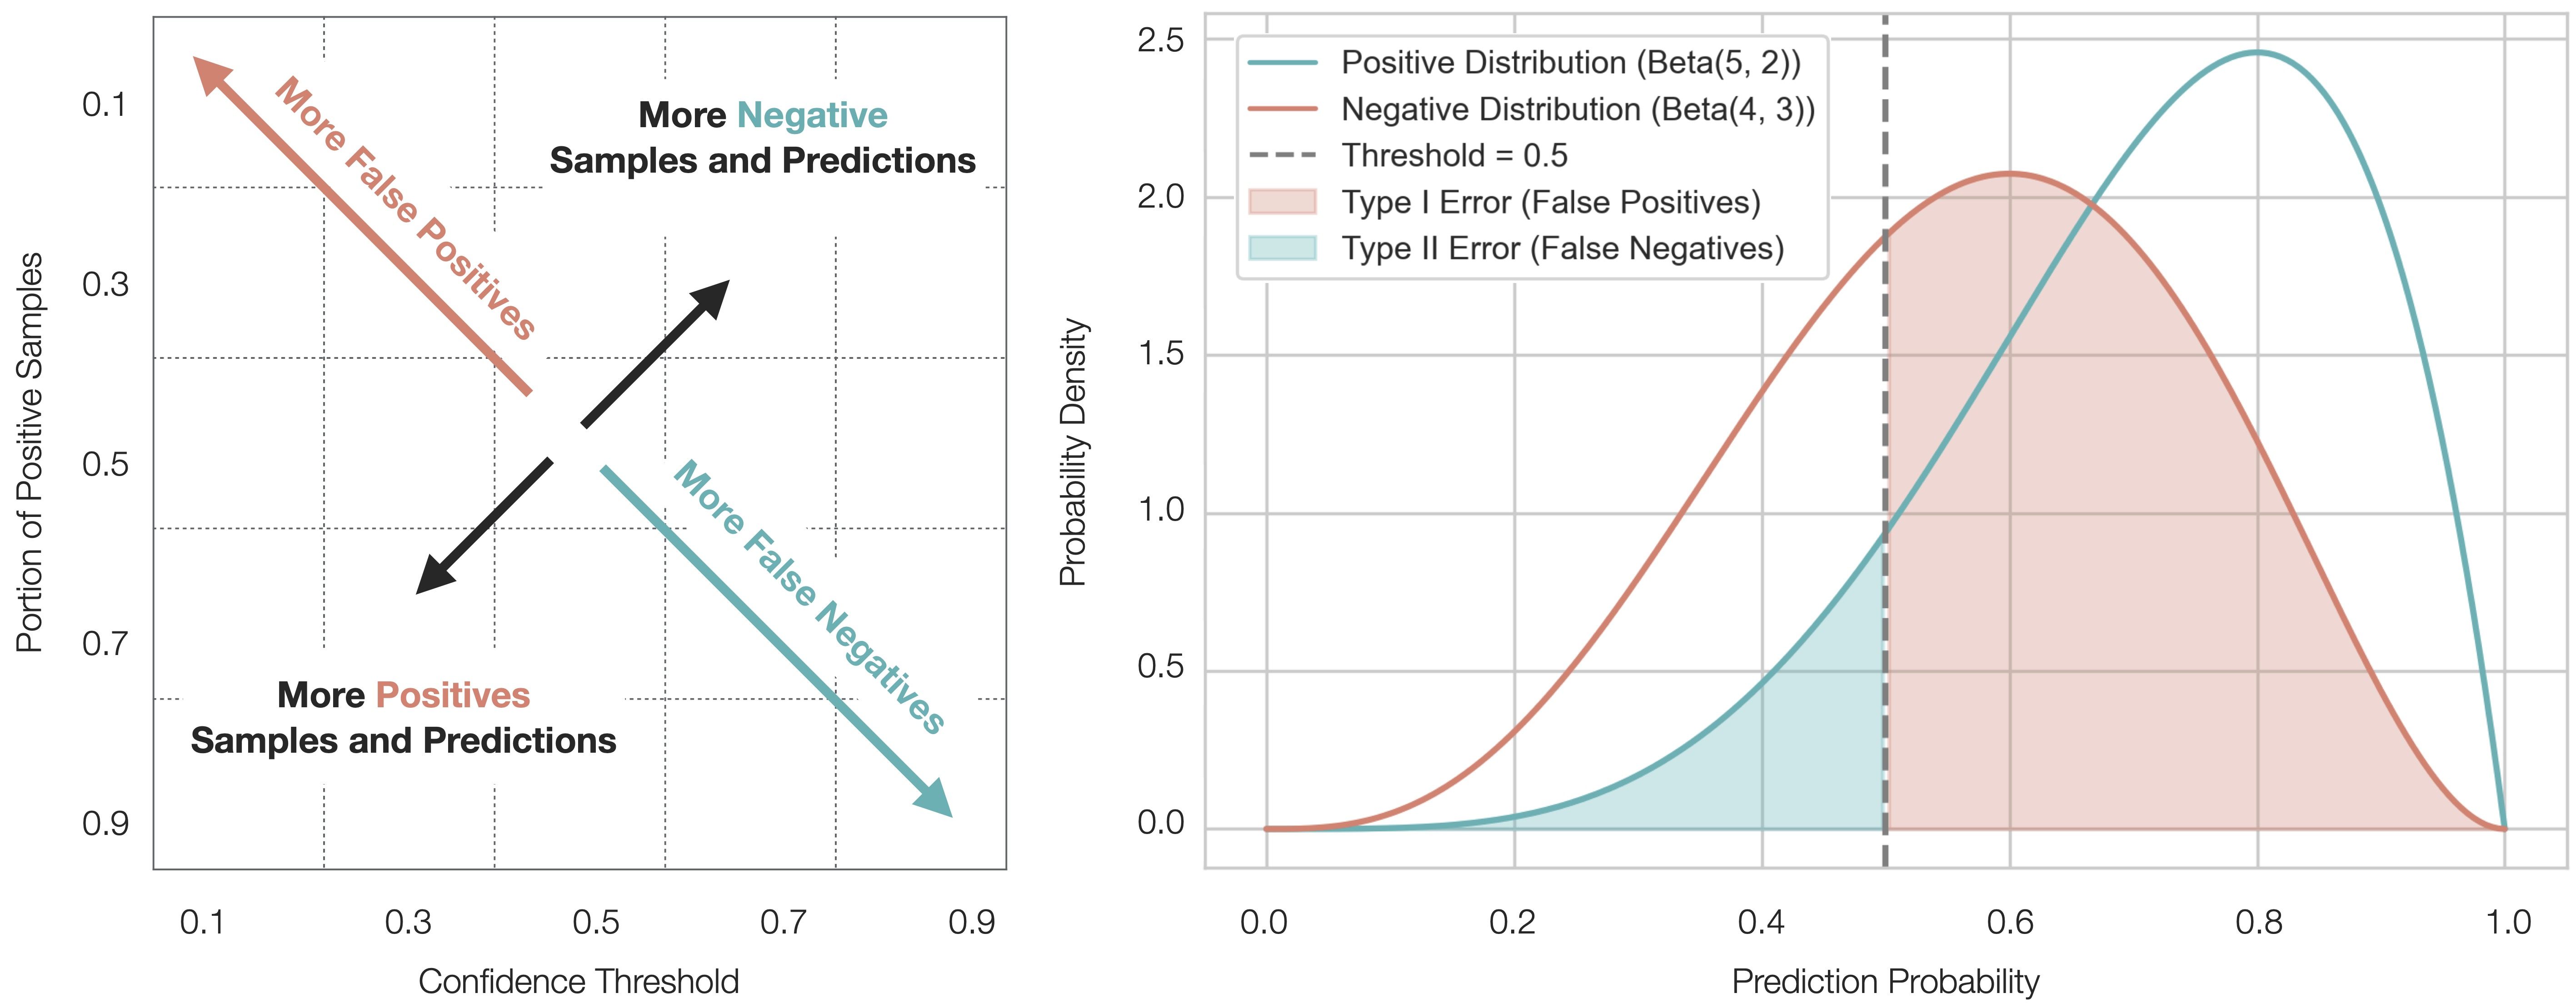
\includegraphics[width=1\textwidth]{fig_5.jpg}
    \caption{Illustration of the simulation design for evaluating classification metrics under varying balance and confidence thresholds. (Left) A 5 × 5 grid of performance metrics, with each cell representing a unique combination of balance level and confidence threshold. (Right) The prediction probability distribution for positive and negative samples.}
    \label{fig:s5_classification}
\end{figure}

The objective of this experiment is to investigate two critical aspects of evaluating binary classification models: the balance between positive and negative samples and the choice of confidence threshold. The experiment aims to explore how these factors influence the performance metrics used to evaluate classification models and to provide insights into the necessity of reporting specific metrics together.



To achieve this, five levels of balance and five levels of confidence thresholds are examined, forming a total of 25 combinations. The inspected levels are $[0.1, 0.3, 0.5, 0.7, 0.9]$ for both balance and confidence thresholds. The balance level is determined by the proportion of positive samples, with a balance level of 0.9 indicating that 90\% of the samples are positive. The confidence threshold is used to dichotomize prediction probabilities, where a higher threshold results in fewer positive predictions by requiring higher certainty for a positive classification. This simulation produces a 5 × 5 grid of performance metrics, where each cell represents a unique combination of balance and confidence threshold (Figure ~\ref{fig:s5_classification}a). The top-left corner of the grid corresponds to a scenario where positive samples are rare, and the model uses a low confidence threshold, resulting in a high false positive rate. In contrast, the bottom-right corner represents a scenario where positive samples are abundant, and the model applies a high confidence threshold, leading to a high false negative rate. This design contrasts these two extreme cases and hence provides a comprehensive evaluation of performance metrics across varying conditions.

The prediction probability, which represents the likelihood of a given sample being classified as positive by the model, is simulated using a beta distribution (Figure ~\ref{fig:s5_classification}b). For positive samples, the prediction probability is drawn from a beta distribution with parameters $\alpha = 5$ and $\beta = 2$, resulting in a peak probability around 0.8. 

For negative samples, the beta distribution has parameters $\alpha = 4$ and $\beta = 3$, with a peak probability around 0.6. This design create a scenario where more false positives are expected than false negatives, as the negative samples have high prediction probabilities that overlap with the positive samples. The shaded area in Figure ~\ref{fig:s5_classification}b represents the overlap between the two distributions, where the confidence threshold is applied. This overlap introduces two types of errors: the region to the right of the threshold intersecting with the negative distribution represents false positives (Type I error), while the region to the left of the threshold intersecting with the positive distribution represents false negatives (Type II error). This setup highlights the trade-off between these error types based on the choice of the confidence threshold.

The metrics evaluated in this experiment include TPR, TNR, FPR, FNR, sensitivity, specificity, precision, recall, accuracy, F1 score, F2 score, and MCC. Although some of these metrics are mathematically equivalent but referred to by different names, this experiment also highlights the reasons why certain metrics are commonly reported together and discusses their complementary roles in evaluating model performance.


\newpage
\section{Results and Discussion}
\subsection{Experiment 1: The Impact of Estimator Choice and Sample Size on Model Evaluation Reliability}

\begin{figure}[H]
    \centering
    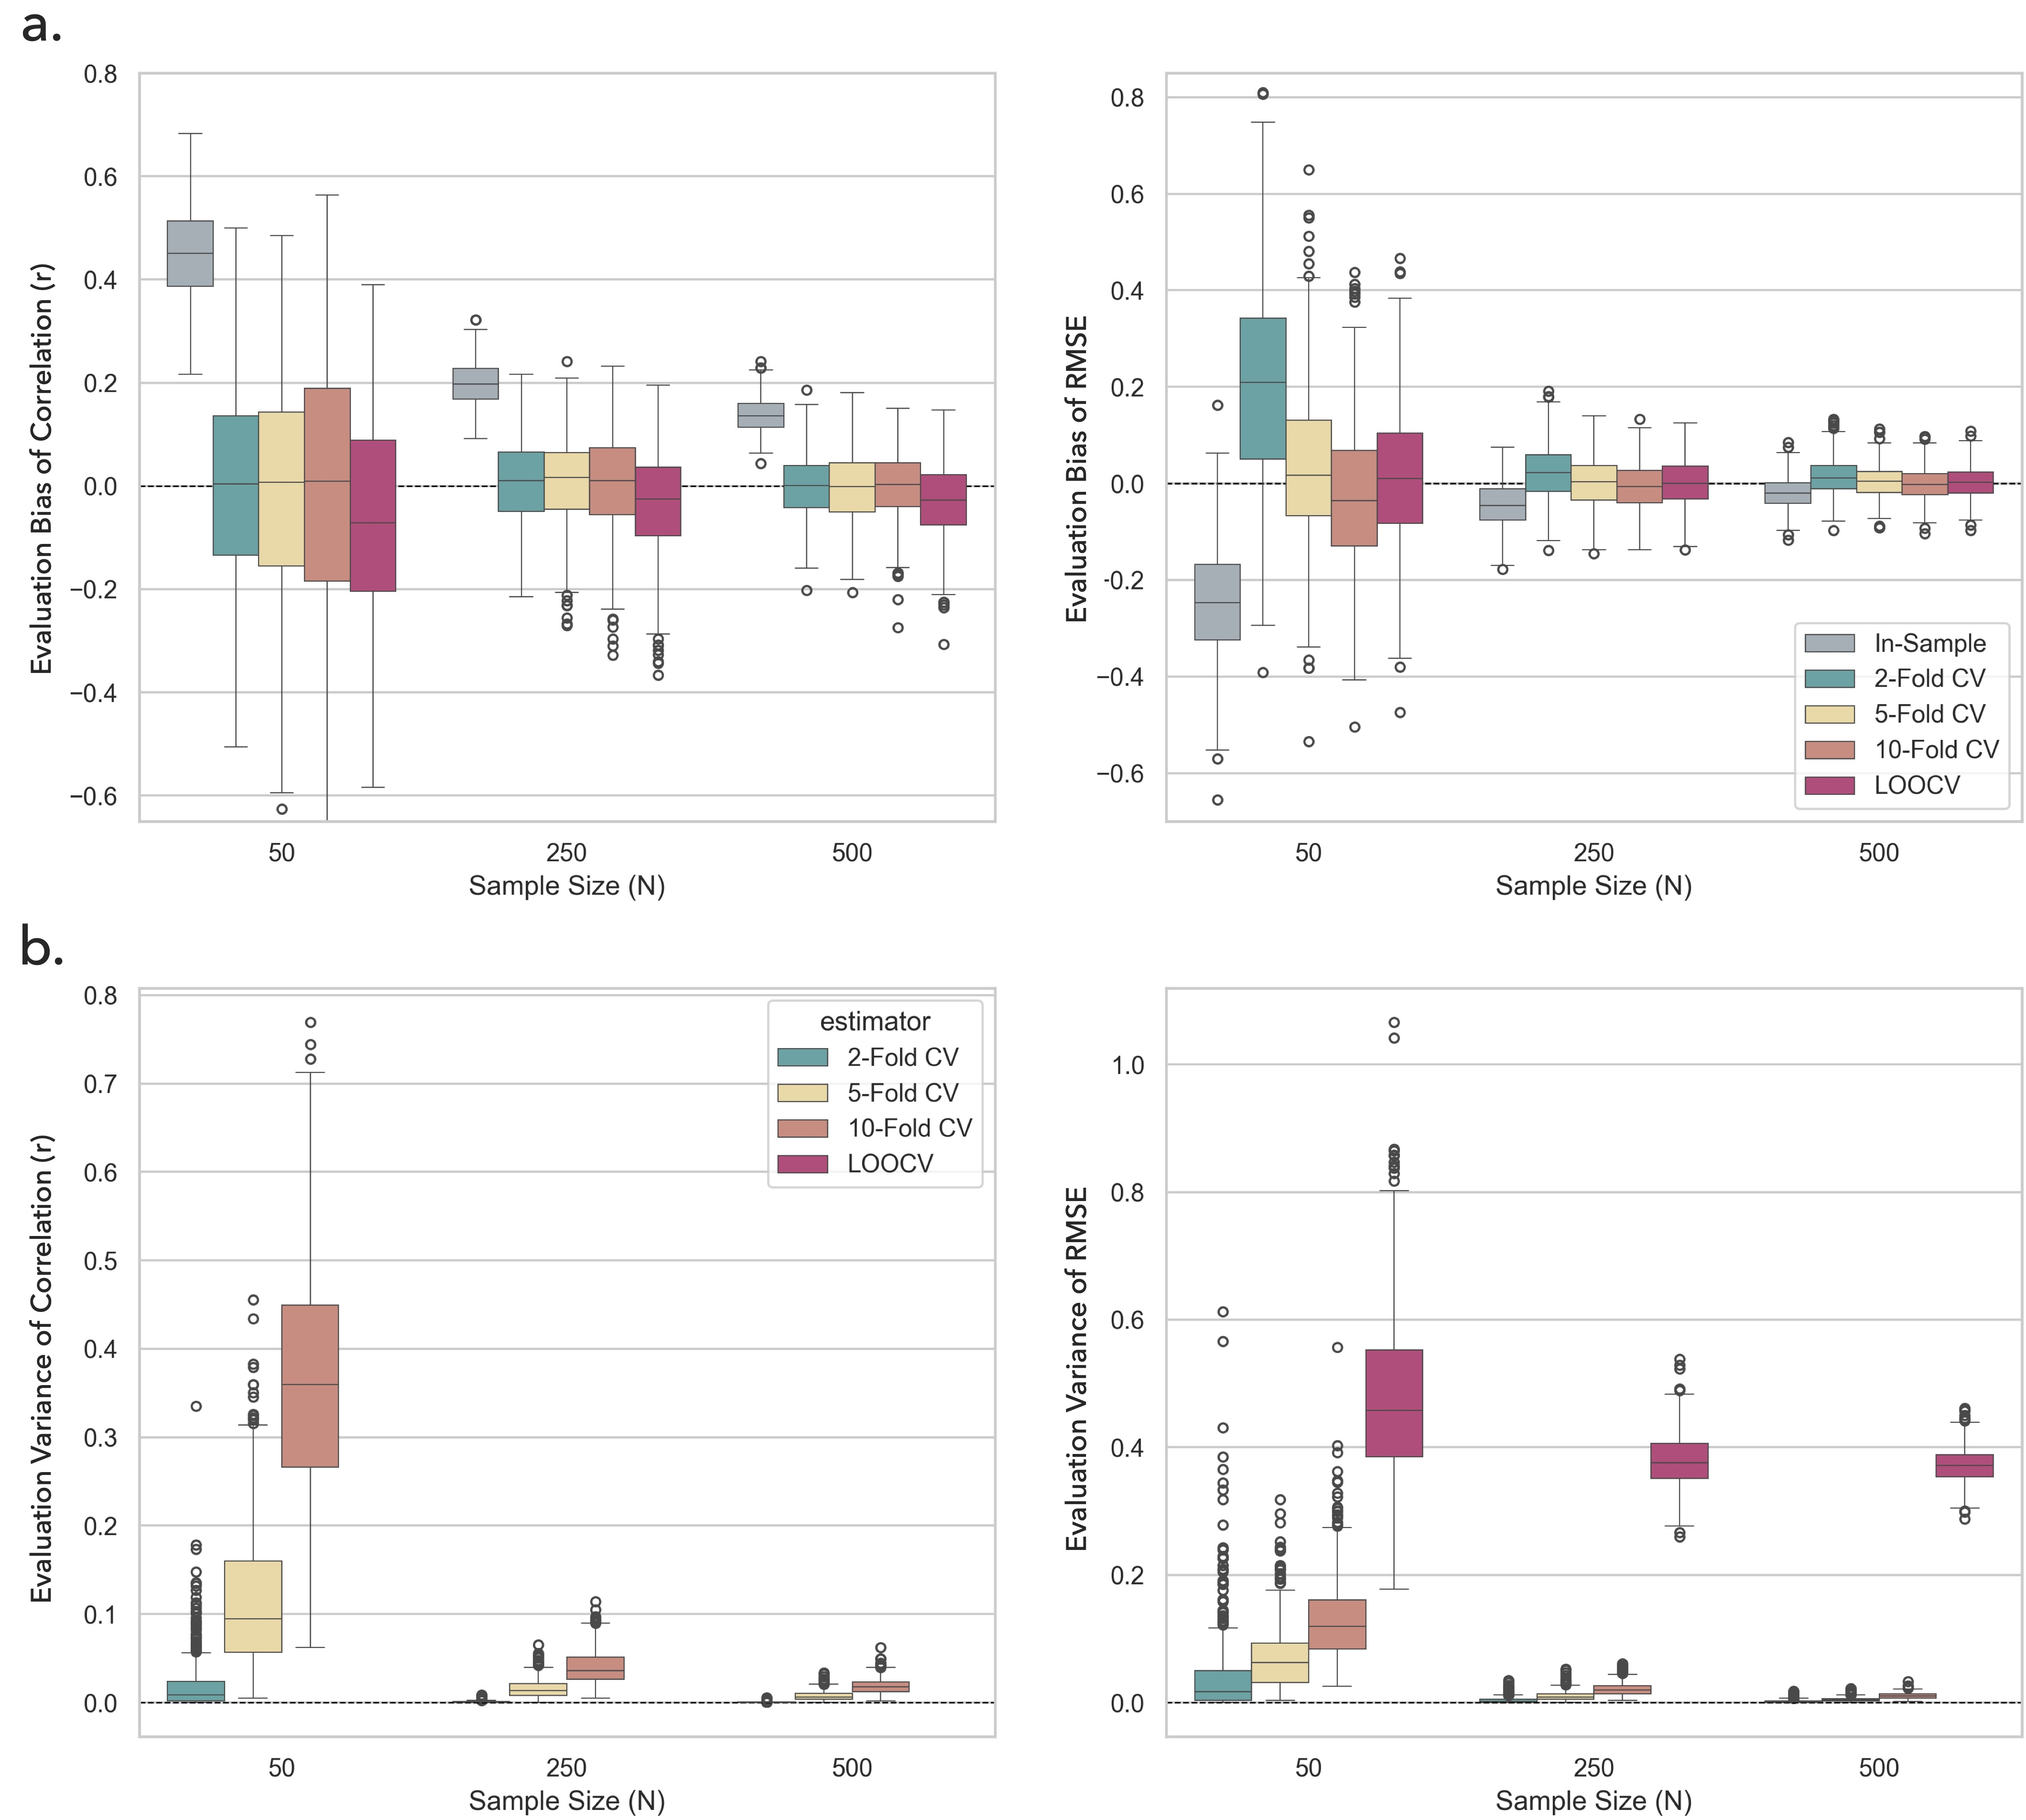
\includegraphics[width=.8\textwidth]{fig_6.jpg}
    \caption{Evaluation bias (8a) and variance (8b) from 500 sampling iterations on the null dataset with 10 feature variables. Multiple performance estimators across different sample sizes were color-coded. Two metrics: $r$ (left) and RMSE (right), were displayed in the column facets.}
    \label{fig:s1_biasvar}
\end{figure}


The results (Figure ~\ref{fig:s1_biasvar}, Table ~\ref{tab:eval_bias}, and Table ~\ref{tab:eval_var}) indicate that both the choice of performance estimator and the sample size notably influence evaluation reliability, which can be decomposed into bias and variance. Although different numbers of folds in CV and LOOCV show no substantial differences in bias, they do affect variance. Specifically, as the number of folds increases, the testing sets become smaller, leading to higher variance. Traditionally, LOOCV has been considered an unbiased estimator for error-based metrics such as $R^2$, RMSE, and MAE. In this experiment, LOOCV generally follows that expectation, except for a few cases at certain sample sizes. Interestingly, when the ratio of sample size to number of features is sufficiently high (e.g., 25 when $N=250$), other $K$-fold estimators can deliver comparable accuracy and bias, offering a more computationally efficient alternative to LOOCV.

However, a key finding emerges with correlation-based metrics (e.g., $r$): LOOCV tends to underestimate model performance and exhibits a pessimistic bias. At $N=250$ and $N=500$, LOOCV’s bias on $r$ can be 10 to 30 times larger than other $K$-fold estimators. In contrast, in-sample (or apparent) estimation, while conventionally deemed the most biased due to information leakage from the testing set, can surprisingly achieve comparable reliability at larger sample sizes. For instance, at $N=250$, the bias of in-sample estimation is only 0.099 for $R^2$ and -0.044 for RMSE, which is less biased than all $K$-fold CV estimators for $R^2$ and less biased than 2-fold CV for RMSE with a smaller sample size of 50. Further examination confirms that a higher number of folds in CV generally reduces bias for error-based metrics (RMSE, MAE) because training sets become more representative of the total data. Yet, correlation-based metrics can display divergent trends under the same conditions. In LOOCV, evaluating a single data point at a time makes its variance particularly evident for RMSE, as single-point predictions inherently fluctuate more. Consequently, across all sample sizes tested, LOOCV consistently exhibits greater variance than lower-fold CV (e.g., 2-fold, 5-fold). Nonetheless, bias and variance across all estimators converge as sample size grows (e.g., $N=500$).

Understanding the potential bias associated with each combination of performance estimator and sample size is critical when comparing similar work across multiple studies. For instance, Haque et al. (2023) reported a classification accuracy of 0.991 using 10-fold cross-validation on a dataset of over 3,000 plant leaf images to train a classifier for identifying potential maize diseases \citep{haque_recognition_2023}. The study claimed that its methodology outperformed other works in terms of model performance. However, one of the cited studies reported an accuracy of 0.925, which was based on a dataset of only 100 images and evaluated using a 70/30 train-test split (approximately equivalent to 3-fold cross-validation) \citep{sibiya_computational_2019}. This comparison is therefore worth questioning, as the performance metrics were derived using different evaluation methods and sample sizes. The apparent performance gap may not reflect differences in the models themselves but rather the evaluation strategies employed.

In conclusion, performance estimation reliability depends strongly on the interplay between the estimation method, the metric in use, and the sample size. Larger sample sizes typically reduce both bias and variance, thereby improving the trustworthiness of model evaluations. While LOOCV often provides less biased estimates for error-based metrics, it can severely underestimate correlation-based metrics and suffers from higher variance. $K$-fold CV methods present a more computationally manageable solution for large datasets and can match LOOCV’s performance when the sample size is sufficiently large relative to the number of features. Ultimately, selecting the most appropriate evaluation strategy should be based on practical considerations—such as available sample size, computational resources, and the specific metrics of interest—to ensure robust and reliable model assessments.


\begin{table}[H]
    \caption{Evaluation bias (mean ± std) for the metrics from 500 sampling iterations. The minimum bias given the same sample size is highlighted in bold. N: training sample size; $r$: Pearson correlation coefficient; $R^2$: coefficient of determination; RMSE: root mean squared error; MAE: mean absolute error. CV: cross-validation; LOOCV: leave-one-out cross-validation.}
    \centering
    \begin{tabular}{lcccc}
        \toprule
        \textbf{Metric} & \textbf{Estimator} & \textbf{N=50} & \textbf{N=250} & \textbf{N=500} \\
        \midrule
        \multirow{5}{*}{$r$} 
            & In-Sample
                & 0.449±0.088
                & 0.198±0.043
                & 0.137±0.033 \\
            & 2-Fold CV
                & \textbf{0.004±0.184}
                & 0.009±0.082
                & -0.001±0.061 \\
            & 5-Fold CV
                & -0.012±0.209
                & 0.006±0.088
                & -0.001±0.067 \\
            & 10-Fold CV
                & -0.011±0.254
                & \textbf{0.003±0.094}
                & \textbf{0.000±0.065} \\
            & LOOCV
                & -0.070±0.203
                & -0.035±0.098
                & -0.031±0.071 \\
        \midrule
        \multirow{5}{*}{$R^2$}
            & In-Sample
                & 0.515±0.207
                & 0.099±0.037
                & 0.053±0.020 \\
            & 2-Fold CV
                & -0.694±0.642
                & -0.044±0.071
                & -0.017±0.034 \\
            & 5-Fold CV
                & -0.401±0.409
                & -0.024±0.049
                & \textbf{-0.007±0.026} \\
            & 10-Fold CV
                & -0.940±0.857
                & -0.046±0.052
                & -0.014±0.024 \\
            & LOOCV
                & \textbf{-0.013±0.256}
                & \textbf{0.009±0.039}
                & 0.008±0.020 \\
        \midrule
        \multirow{5}{*}{RMSE}
                & In-Sample
                    & -0.244±0.116
                    & -0.044±0.044
                    & -0.020±0.032 \\
                & 2-Fold CV
                    & 0.215±0.226
                    & 0.022±0.056
                    & 0.013±0.036 \\
                & 5-Fold CV
                    & 0.035±0.158
                    & 0.002±0.047
                    & 0.004±0.033 \\
                & 10-Fold CV
                    & -0.024±0.149
                    & -0.006±0.046
                    & \textbf{-0.001±0.033} \\
                & LOOCV
                    & \textbf{0.012±0.144}
                    & \textbf{0.001±0.046}
                    & 0.003±0.033 \\
        \midrule
        \multirow{5}{*}{MAE}
                & In-Sample
                    & -0.195±0.096
                    & -0.037±0.037
                    & -0.017±0.028 \\
                & 2-Fold CV
                    & 0.180±0.190
                    & 0.017±0.047
                    & 0.010±0.030 \\
                & 5-Fold CV
                    & 0.049±0.134
                    & 0.004±0.039
                    & 0.003±0.028 \\
                & 10-Fold CV
                    & 0.022±0.127
                    & 0.002±0.038
                    & 0.002±0.028 \\
                & LOOCV
                    & \textbf{0.011±0.119}
                    & \textbf{-0.001±0.038}
                    & \textbf{0.001±0.028} \\
        \bottomrule
    \end{tabular}
    \label{tab:eval_bias}
\end{table}
    

\begin{table}[H]
    \caption{Evaluation variance (mean ± std) for the metrics from 500 sampling iterations. The minimum variance given the same sample size is highlighted in bold. N: training sample size; $r$: Pearson correlation coefficient; $R^2$: coefficient of determination; RMSE: root mean squared error; MAE: mean absolute error. CV: cross-validation; LOOCV: leave-one-out cross-validation.}
    \centering
    \begin{tabular}{lcccc}
        \toprule
        \textbf{Metric} & \textbf{Estimator} 
            & \textbf{N=50} & \textbf{N=250} & \textbf{N=500} \\
        \midrule
        \multirow{3}{*}{$r$}
            & 2-Fold CV
                & \textbf{0.019±0.030} 
                & \textbf{0.001±0.001}
                & \textbf{0.000±0.001} \\
            & 5-Fold CV
                & 0.117±0.081
                & 0.016±0.011
                & 0.008±0.005 \\
            & 10-Fold CV
                & 0.362±0.131
                & 0.040±0.019
                & 0.019±0.009 \\          
        \midrule
        \multirow{3}{*}{$R^2$}
            & 2-Fold CV
                & 0.859±2.876
                & \textbf{0.003±0.006}
                & \textbf{0.001±0.001} \\
            & 5-Fold CV
                & \textbf{0.743±1.391}
                & 0.008±0.009
                & 0.002±0.002 \\
            & 10-Fold CV
                & 7.164±37.486
                & 0.018±0.019
                & 0.003±0.002 \\
               
        \midrule
        \multirow{4}{*}{RMSE}
            & 2-Fold CV
                & \textbf{0.041±0.068}
                & \textbf{0.004±0.005}
                & \textbf{0.002±0.003} \\
            & 5-Fold CV
                & 0.070±0.050
                & 0.010±0.008
                & 0.005±0.004 \\
            & 10-Fold CV
                & 0.130±0.067
                & 0.021±0.010
                & 0.010±0.005 \\
            & LOOCV
                & 0.477±0.131
                & 0.379±0.041
                & 0.371±0.029 \\         
        \midrule
        \multirow{4}{*}{MAE}
            & 2-Fold CV
                & \textbf{0.030±0.053}
                & \textbf{0.003±0.003}
                & \textbf{0.001±0.002} \\
            & 5-Fold CV
                & 0.052±0.039
                & 0.008±0.005
                & 0.004±0.003 \\
            & 10-Fold CV
                & 0.100±0.052
                & 0.015±0.007
                & 0.008±0.004 \\
            & LOOCV
                & 0.477±0.131
                & 0.379±0.041
                & 0.371±0.029 \\
        \bottomrule
    \end{tabular}
    \label{tab:eval_var}
\end{table}

\subsection{Experiment 2: Misuse of Model Selection Can Lead to Over-Optimistic Performance Estimates}

\begin{figure}[H]
    \centering
    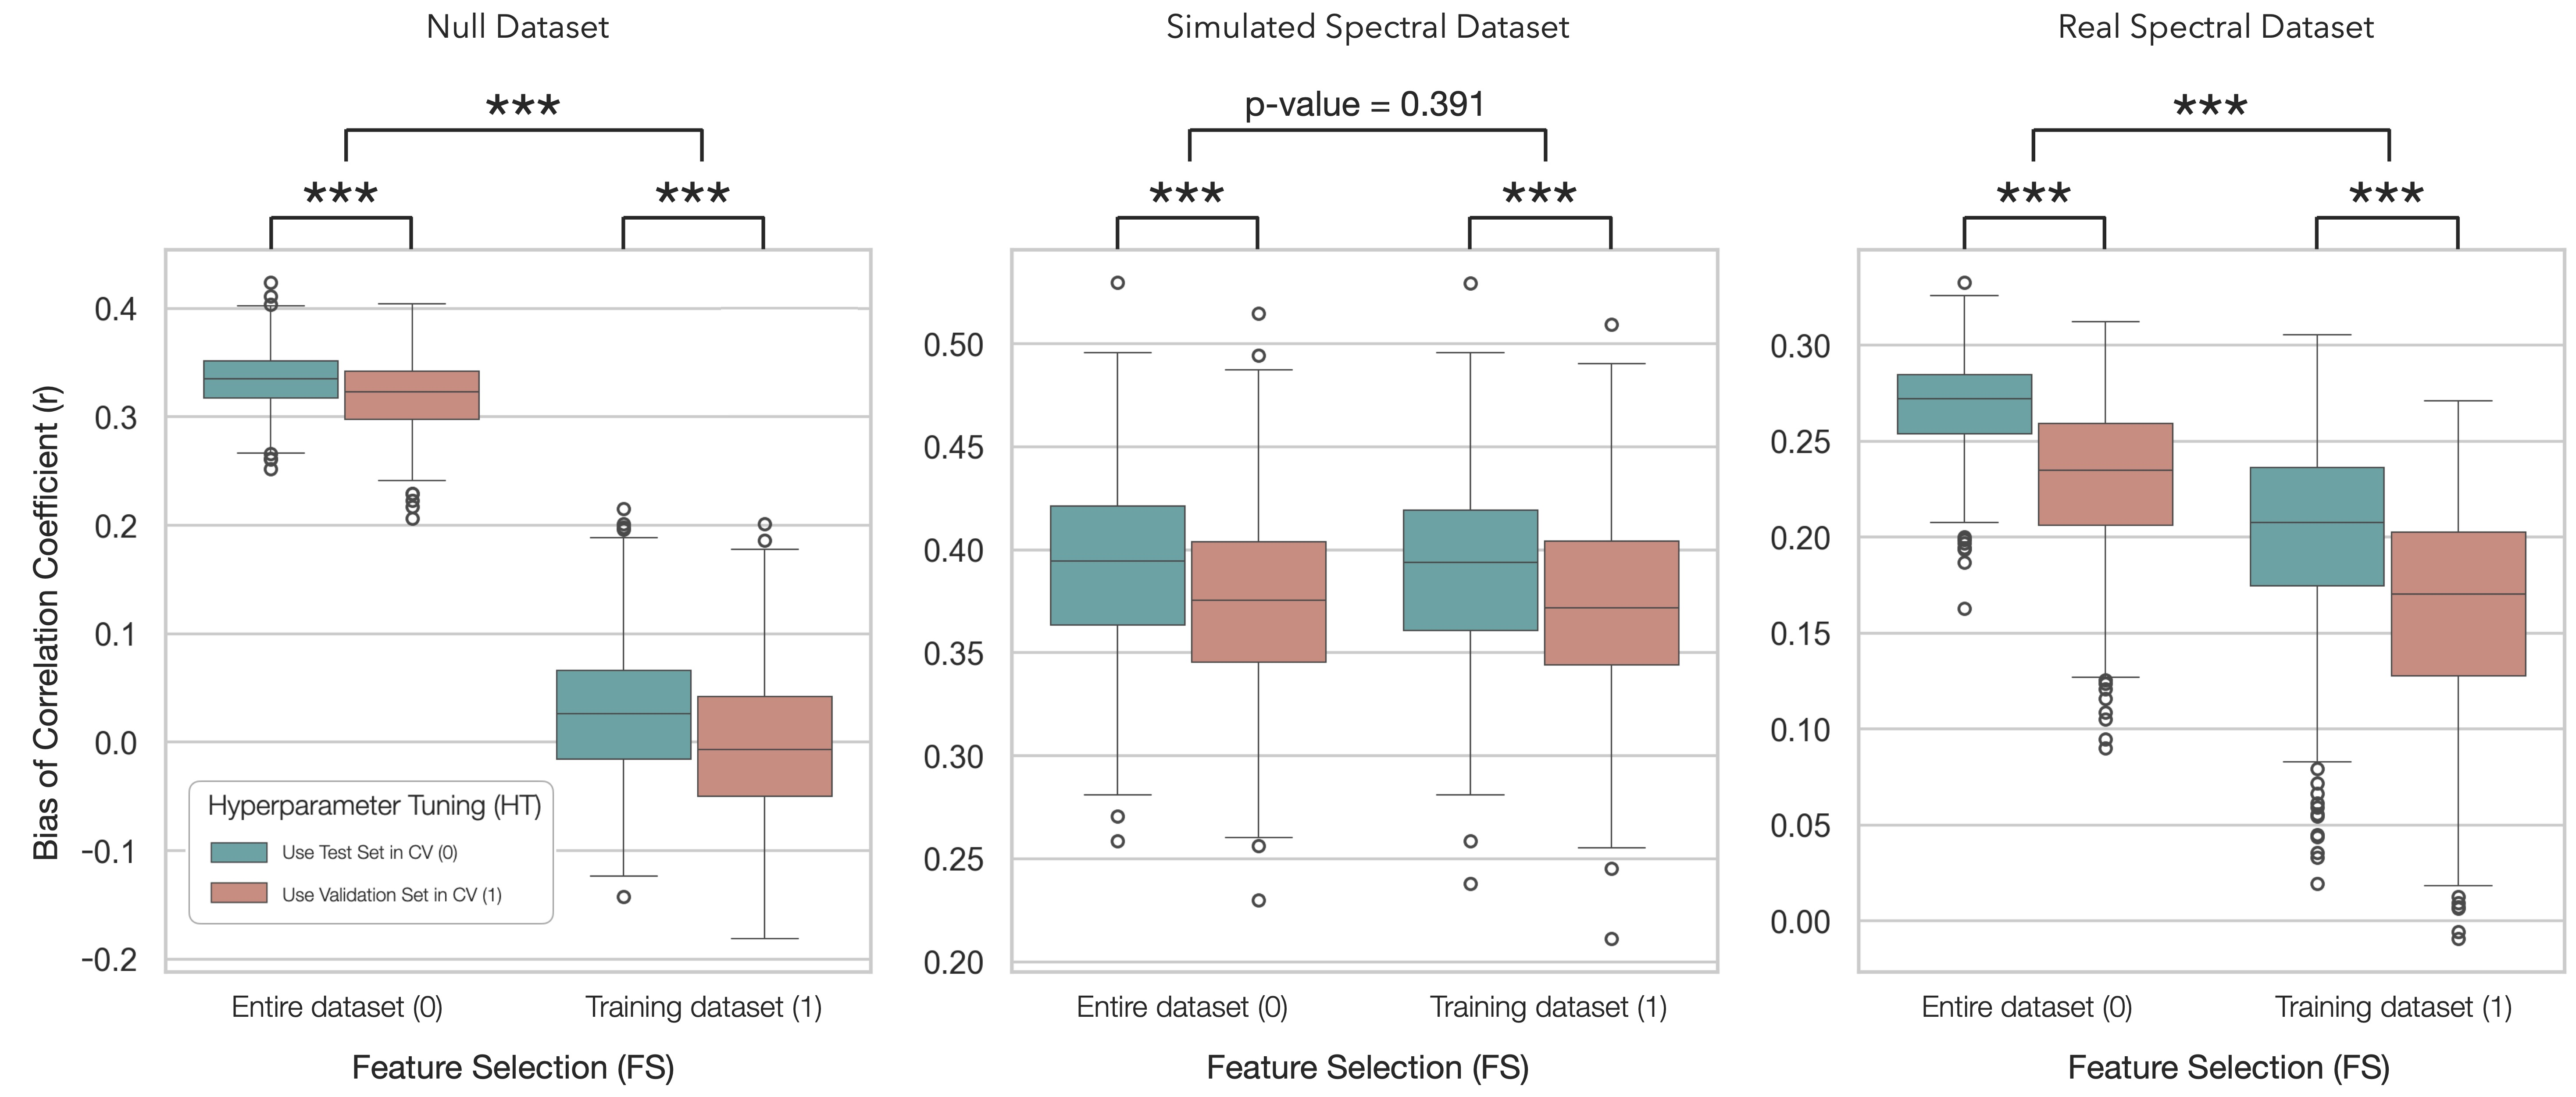
\includegraphics[width=1\textwidth]{fig_7.jpg}
    \caption{The evaluation bias of the four combinations of model selection strategies: “FS=0; HT=0”, “FS=0; HT=1”, “FS=1; HT=0”, “FS=1; HT=1” across three datasets. The significance level of the difference between the two strategies is noted as *** < 0.00001.}
    \label{fig:s2_results}
\end{figure}

With the exception of the feature selection procedure in the simulated spectral dataset, all other procedures that erroneously incorporate the testing set into the model selection process substantially inflate evaluation bias (Figure~\ref{fig:s2_results} and Table~\ref{tab:anova_r}). However, the magnitude of this inflation varies across datasets. In the null dataset, incorrectly performing feature selection leads to roughly a 30\% performance inflation; on the real dataset, a similar practice results in a 6\% inflation. By contrast, the simulated spectral dataset shows no measurable inflation, with only a negligible 0.02\% change in r. This minimal effect may stem from the degree to which the selected features contribute to predictive accuracy. If a model’s performance is comparable to that obtained through random feature selection, then leveraging the testing set for feature selection does not necessarily boost performance. Such a scenario is more plausible in datasets with high multicollinearity, where multiple features correlate strongly, making any subset of features effectively representative of the entire feature space.

On the other hand, using the entire dataset to perform hyperparameter tuning substantially inflates performance in all three datasets—by approximately 2.5\% in the null dataset, 1.5\% in the simulated spectral dataset, and nearly 4\% in the real spectral dataset. It is worth noting that these estimates arise from a relatively small search space of only six hyperparameter combinations. In contemporary machine learning, hyperparameter spaces can be far larger, especially for deep learning models in which the architectures themselves are highly configurable, involving potentially millions of parameters. Even minor alterations (e.g., changing the kernel size in a convolutional layer) may markedly affect model performance in such complex settings \citep{zoph_neural_2017}.

Model selection practices are critical in many precision agricultural applications. It is important to note that feature selection is not entirely prohibited from using the entire dataset, especially when employing unsupervised feature selection methods, such as the successive projections algorithm (SPA) \citep{soares_successive_2013}. These methods consider feature redundancy and select the most informative features without incorporating information from the target variable in the testing set. For example, Zhang et al. (2019) leveraged ground-based hyperspectral sensors to detect weed species in rice fields \citep{zhang_automated_2019}. Even after preprocessing and discarding spectral bands with high fluctuations due to hardware limitations, 470 bands remained for consideration. The SPA method was employed to select the most informative bands for the prediction task, ultimately identifying six key bands that also match the past literature on weed detection. This procedure is considered unbiased, as the feature selection was not explicitly performed to maximize model performance.

The same study demonstrated good practices in hyperparameter tuning. Within each training fold, a nested 5-fold cross-validation was implemented to identify the optimal hyperparameter combinations. For the random forest model, the number of trees and the spectral bands considered for splits were tuned during classifier development. Similarly, for the SVM model, the best regularization parameter $C$ and kernel function were identified to avoid overfitting. Other studies have adopted similar practices. For instance, Shahinfar et al. (2019) used a large dataset of sheep growth management records to predict carcass traits, including birth weight, age at slaughter, and breeding values for fat composition from ancestors \citep{shahinfar_prediction_2019}. Given the large feature space, careful hyperparameter tuning was essential to prevent overfitting. Shahinfar et al. employed nested cross-validation to select the optimal number of decision trees and bootstrap samples for the random forest model. These examples illustrate the importance of rigorous feature selection and hyperparameter tuning to enhance model reliability and generalizability in precision agricultural studies.

Collectively, these findings underscore the importance of rigorous CV practices in model selection, particularly for feature selection and hyperparameter tuning, to achieve accurate performance estimates and robust generalizability in predictive modeling.

\subsection{Experiment 3: Overlooking Experimental Block Effects Can Lead to Biased Model Performance Estimates}

\begin{figure}[H]
    \centering
    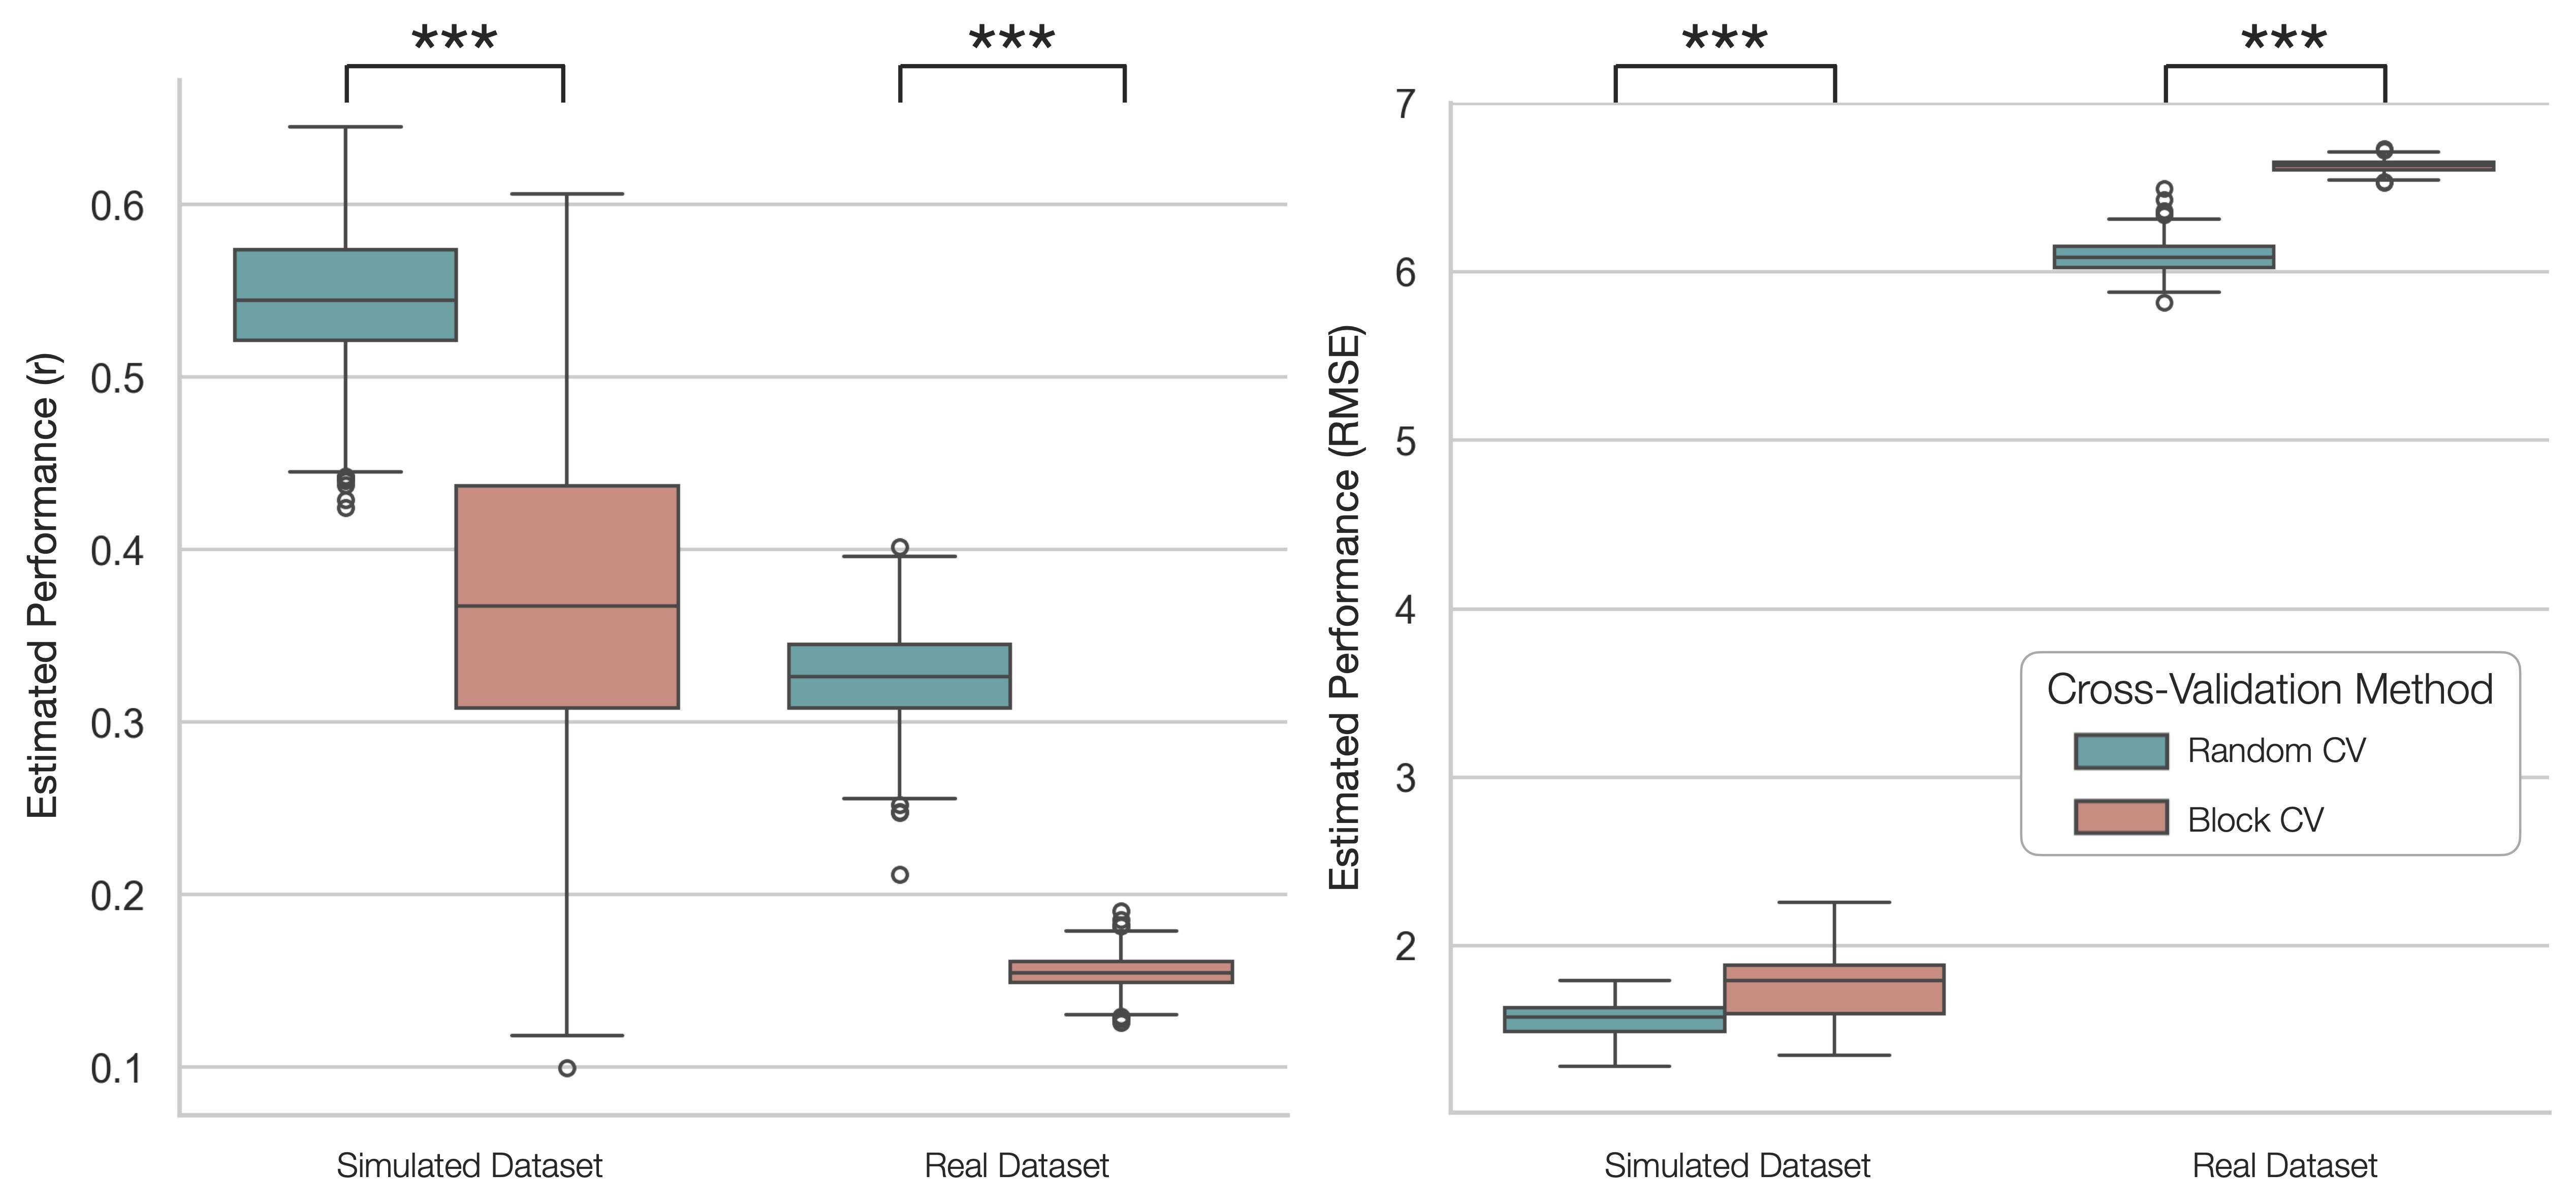
\includegraphics[width=1\textwidth]{fig_8.jpg}
    \caption{Bias in model performance estimation by Block CV and Random CV across 1000 iterations. The dashed line represents the null hypothesis that the mean performance estimate is zero. The significance level is noted as *** < 0.00001.}
    \label{fig:s3_results}
\end{figure}

Performance inflation is evident in both the simulated and real spectral datasets, which inherently exhibit seasonal variation as block effects (Figure~\ref{fig:s3_results} and Table~\ref{tab:anova_all}). Ignoring this seasonal variation leads to a notable overestimation of model performance, as reflected by a 17.5\% bias in r for the simulated dataset and 17.1\% for the real dataset. A similar pattern emerges for RMSE, with a 15.5\% bias in the simulated dataset and an 11.1\% bias in the real dataset. The ANOVA results further support these findings, since all four tests show significant differences (p-value < 0.001) between the two methods on the estimated model performance.

St-Pierre (2001) made a similar observation when comparing datasets collected from different studies conducted under distinct time periods or environmental conditions \citep{st-pierre_invited_2001}. The distinctness often manifests in differences in variance or value scales, complicating comparisons in the literature. St-Pierre defined this phenomenon as the “study effect,” recommending that it be calibrated as a random variable instead of a fixed variable in a linear mixed model. It is because these study effects are unobserved until the data is collected, fitting these effects as random variables allows for the calibration of a broader set of study effects, including those that are unobserved. The author advocated for calibrating the study variation before making any inferences from the dataset, which parallels the need to calibrate the seasonal variation in prediction modeling to alleviate the overestimation bias observed in random CV.

Similar discussion are found in maize breeding. Predicting hybrid yield performance for future years or seasons has been a challenge. De Oliveira et al. (2020) estimated hybrid performance across multiple years and compared two CV systems \citep{de_oliveira_genomic_2020}. The first system used random splits of the available hybrids into validation folds, while the second employed year-based splits, which is an approach akin to block CV as advocated in this study. The results showed substantial performance differences of up to 0.4 in $r$ across years, underscoring the impact of properly accounting for temporal effects. Since seasons are inherently random effects that cannot be fully observed in historical datasets (as no two seasons are identical in their environmental responses to yield), a common strategy to address this issue is to quantify year-to-year variation using quantitative variables rather than directly modeling the seasonal effect. In crop modeling, such variables are referred to as environmental covariates, which decompose environmental variability into measurable components like temperature, humidity, and soil moisture. For instance, Cruz et al. (2023) incorporated 183 environmental covariates, including cumulative thermal time, soil water evaporation, leaf area index, and daily infiltration, into their prediction models \citep{lopez-cruz_leveraging_2023}. By estimating the effects of these covariates, researchers can address the missing information from unseen seasonal variations and mitigate the performance drop when transitioning from random CV to block CV.

These observations emphasize the importance of closely examining identifiable sources of variation in experiments and aligning evaluation strategies with the model’s intended real-world application. Variations, such as seasonal block effects, can simultaneously influence both predictive features and response variables. If a model is intended for deployment in a new block, such as a future season for which no prior information is available, using block CV is critical to ensure the evaluation results in generalizability. Conversely, for models designed for a closed environment where all possible blocks are represented, random CV may offer a more efficient evaluation strategy.

\subsection{Experiment 4: Characteristics of Metrics in Regression Tasks}

\begin{figure}[H]
    \centering
    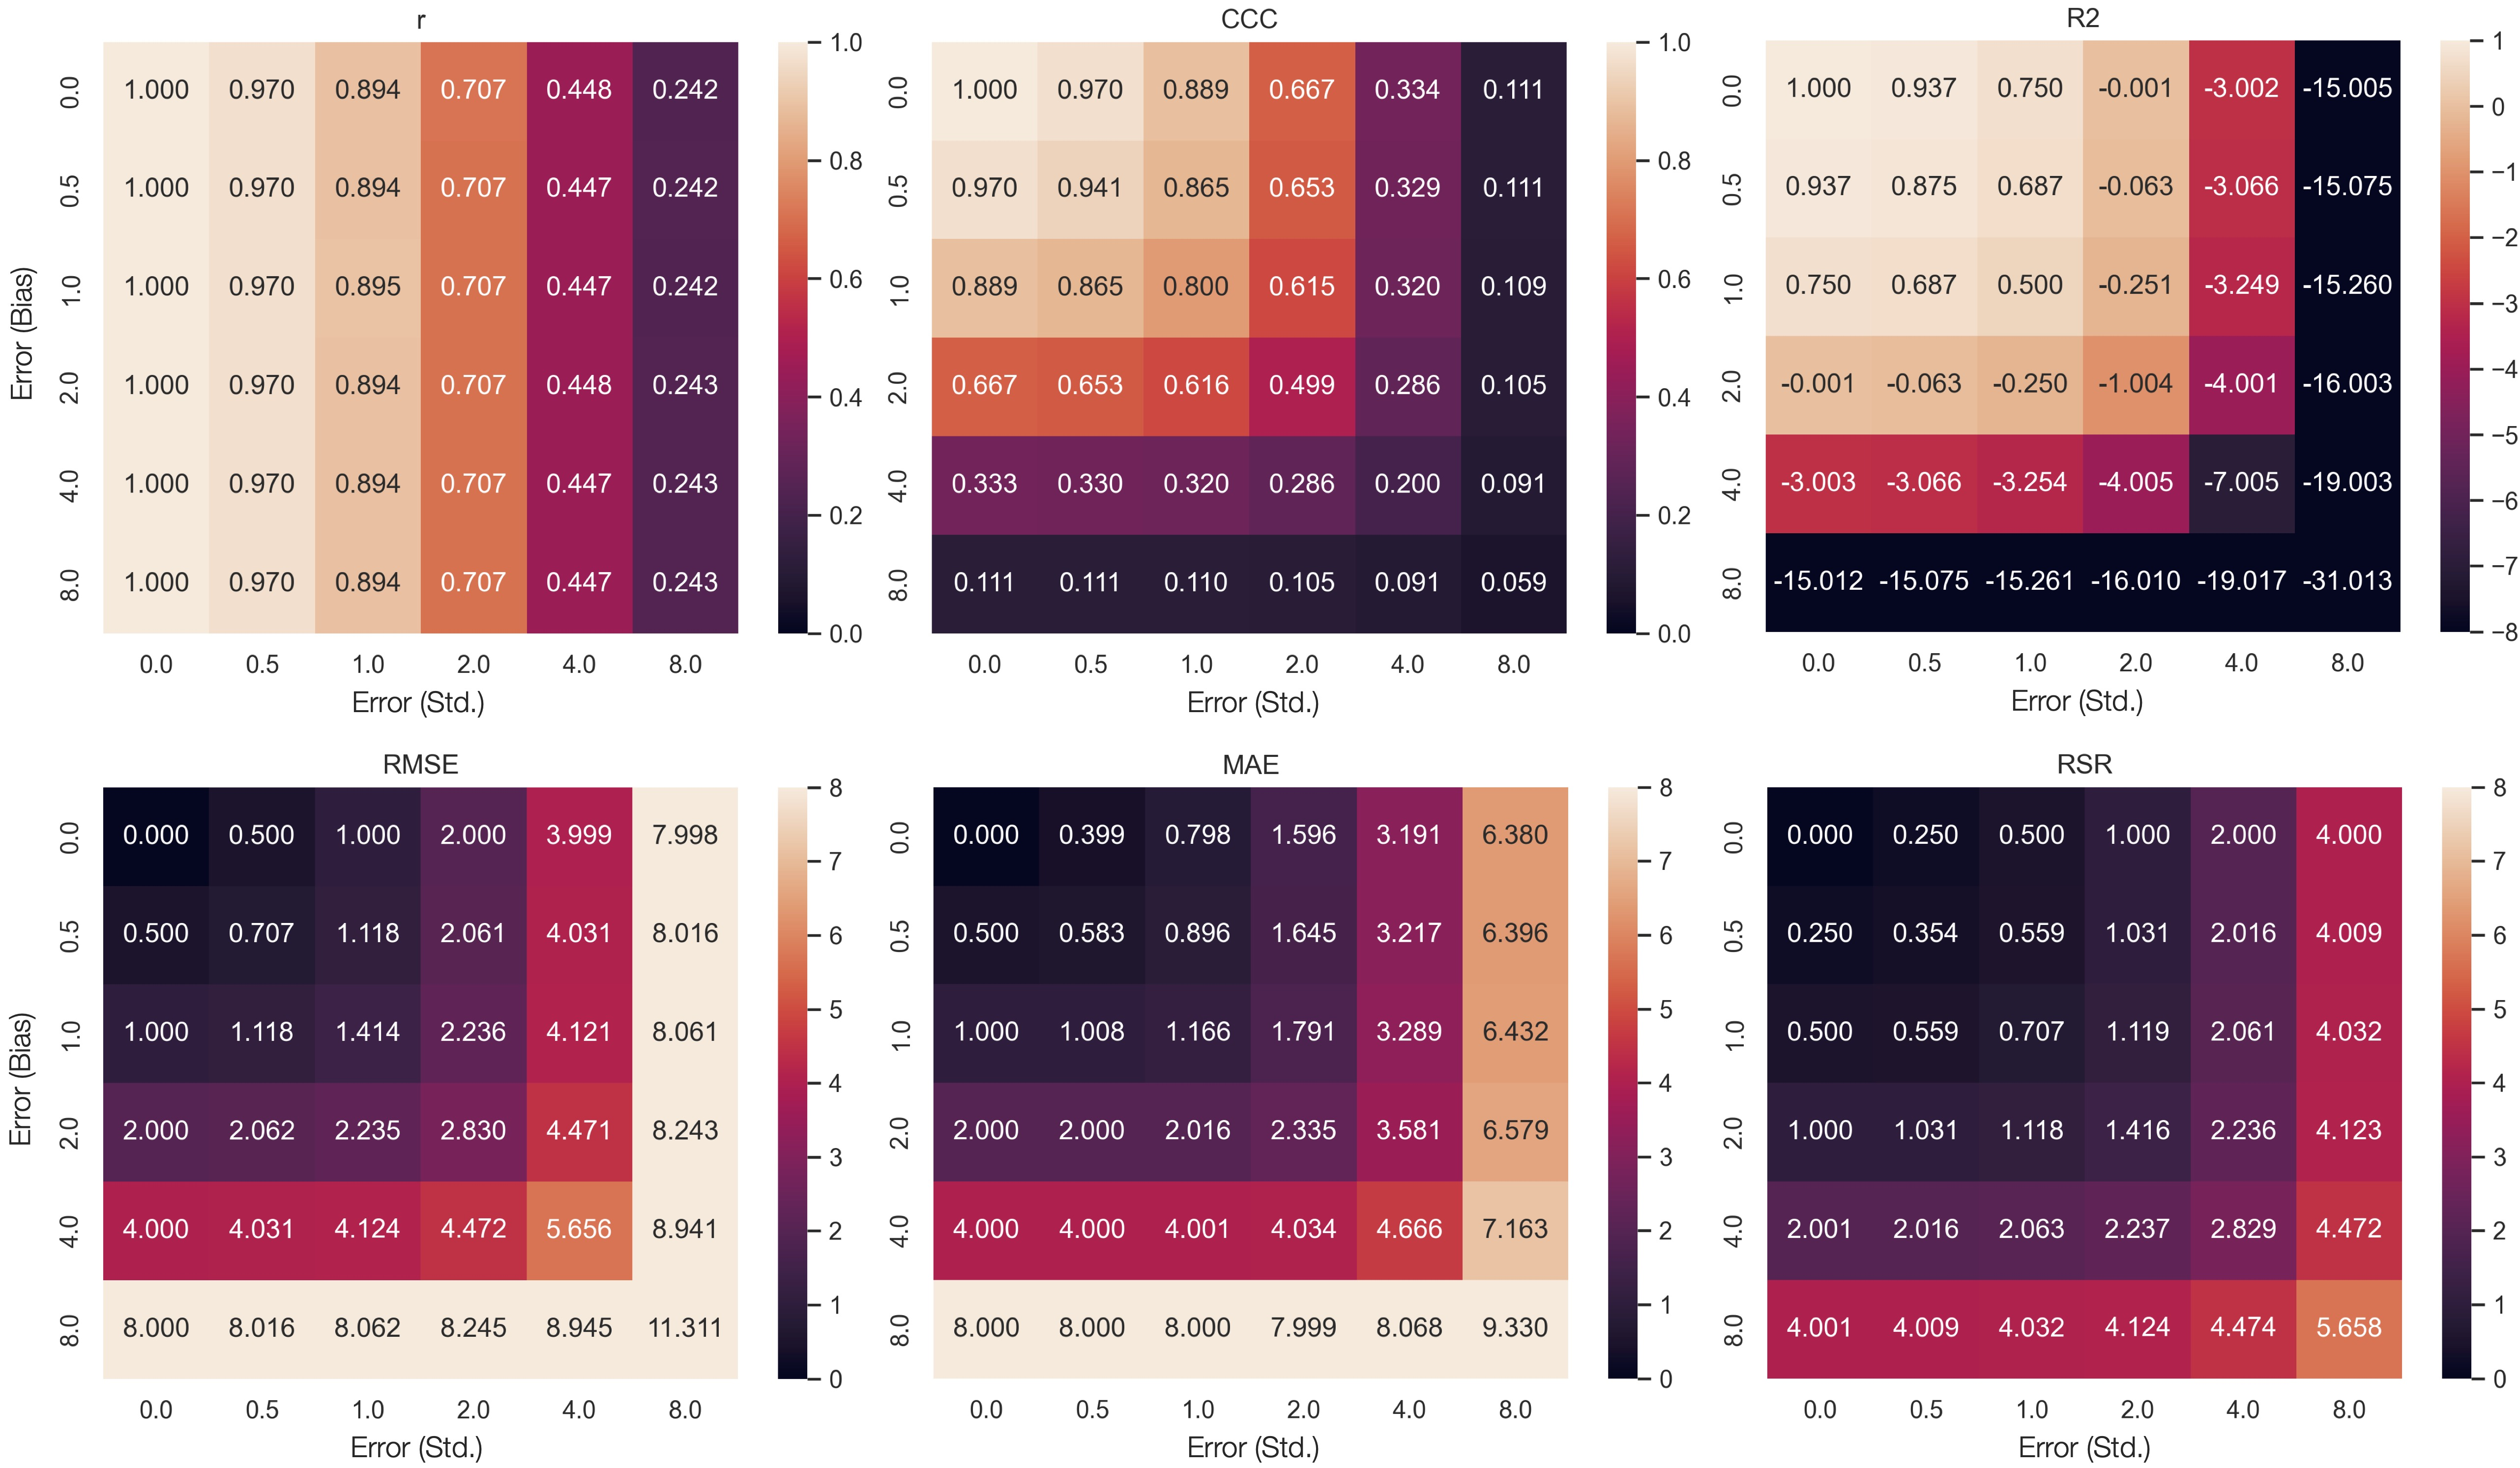
\includegraphics[width=1\textwidth]{fig_9.jpg}
    \caption{Heatmaps illustrating various metrics as functions of the bias and standard deviation (Std.) of the prediction error in a regression task, where the ground truth values have a Std. of 4.}
    \label{fig:s4_reg}
\end{figure}

Metrics in regression tasks exhibit distinct trends in response to various combinations of error bias and variance (Figure \ref{fig:s4_reg}). Except for $r$ and MAE, all metrics demonstrate symmetric responses in the grid matrix, supporting the trade-off relationship between bias and variance. For instance, $R^2$ consistently shows a value of 0.75 at the positions (1, 4) and (4, 1), indicating that a model with zero bias and variance of 2 achieves the same $R^2$ as a model with bias of 2 and zero variance.

Both $r$ and CCC are linearity-based metrics that assess the correlation between predicted and actual values, yet they exhibit different trends in the heatmap. Since $r$ is standardized by the standard deviation of both predicted and actual values, it is entirely invariant to bias errors, which reflect the scale of the prediction error. In contrast, CCC is sensitive to both bias and variance, offering a more comprehensive evaluation of correlation. In this experiment, CCC also provides better interpretability compared to $r$. Specifically, when \text{CCC} > 0.5, the total squared error (i.e., the sum of squared bias and variance) does not exceed $4 + 4 = 8$, which is twice the ground truth variance ($2^2 = 4$). Furthermore, when \text{CCC} > 0.8, the error is guaranteed to be less than the ground truth variance. Unlike the ambiguous interpretation of r, these benchmarks provide a straightforward guideline for translating the correlation concept into the scale of prediction errors.

$R^2$ is a widely used metric in the machine learning community and offers good interpretability. When $R^2 = 0$, it indicates that the model performs no better than the mean prediction. In the heatmap, this is evident at positions (4, 1) and (1, 4), where the prediction error equals the ground truth variance. Additionally, when $R^2 = -1$, it suggests the prediction error exceeds the mean prediction error by one unit of the ground truth variance, as seen at position (4, 4), where both bias and variance errors are 2, resulting in a total squared error of 8 (twice the ground truth variance). Although $R^2$ shares similar interpretability with CCC, it inflates rapidly in the presence of outliers. For example, when the bias or variance error increases from 4 to 8, $R^2$ drops dramatically from -3 to -15. In contrast, CCC decreases only by 0.22 under the same conditions, maintaining a range between 0 and 1, which makes it more stable and comparable across different prediction contexts.

Error-based metrics like RMSE and MAE are often compared for their robustness to outliers. Due to the squared error term in RMSE, it is more sensitive to large prediction errors. Interestingly, when analyzing their response to increases in bias error, RMSE and MAE exhibit identical trends: a 1-unit increase in bias error results in a 1-unit increase in both metrics. However, differences emerge along the variance error axis, where MAE increases by only 0.8 units per unit increase in variance error, whereas RMSE increases by 1 unit. This indicates that MAE is more robust to variance-related errors than RMSE, making it better suited for handling outlier predictions.

RSR, on the other hand, standardizes RMSE by the standard deviation of the ground truth values. In this experiment, where the ground truth values were generated from a normal distribution with a standard deviation of 2, RSR serves as a direct comparison to RMSE. While RMSE reflects the original error scale, RSR normalizes the error scale to the ground truth variance, resulting in values that are always half those of RMSE. This property makes RSR an excellent metric for comparing model performance across multiple datasets with varying variance levels. RSR provides a uniform standard for performance evaluation while retaining the capability to capture error amplitude, which linearity-based metrics like $r$ and CCC lack.

\subsection{Experiment 5: Characteristics of Metrics in Classification Tasks}

\begin{figure}[H]
    \centering
    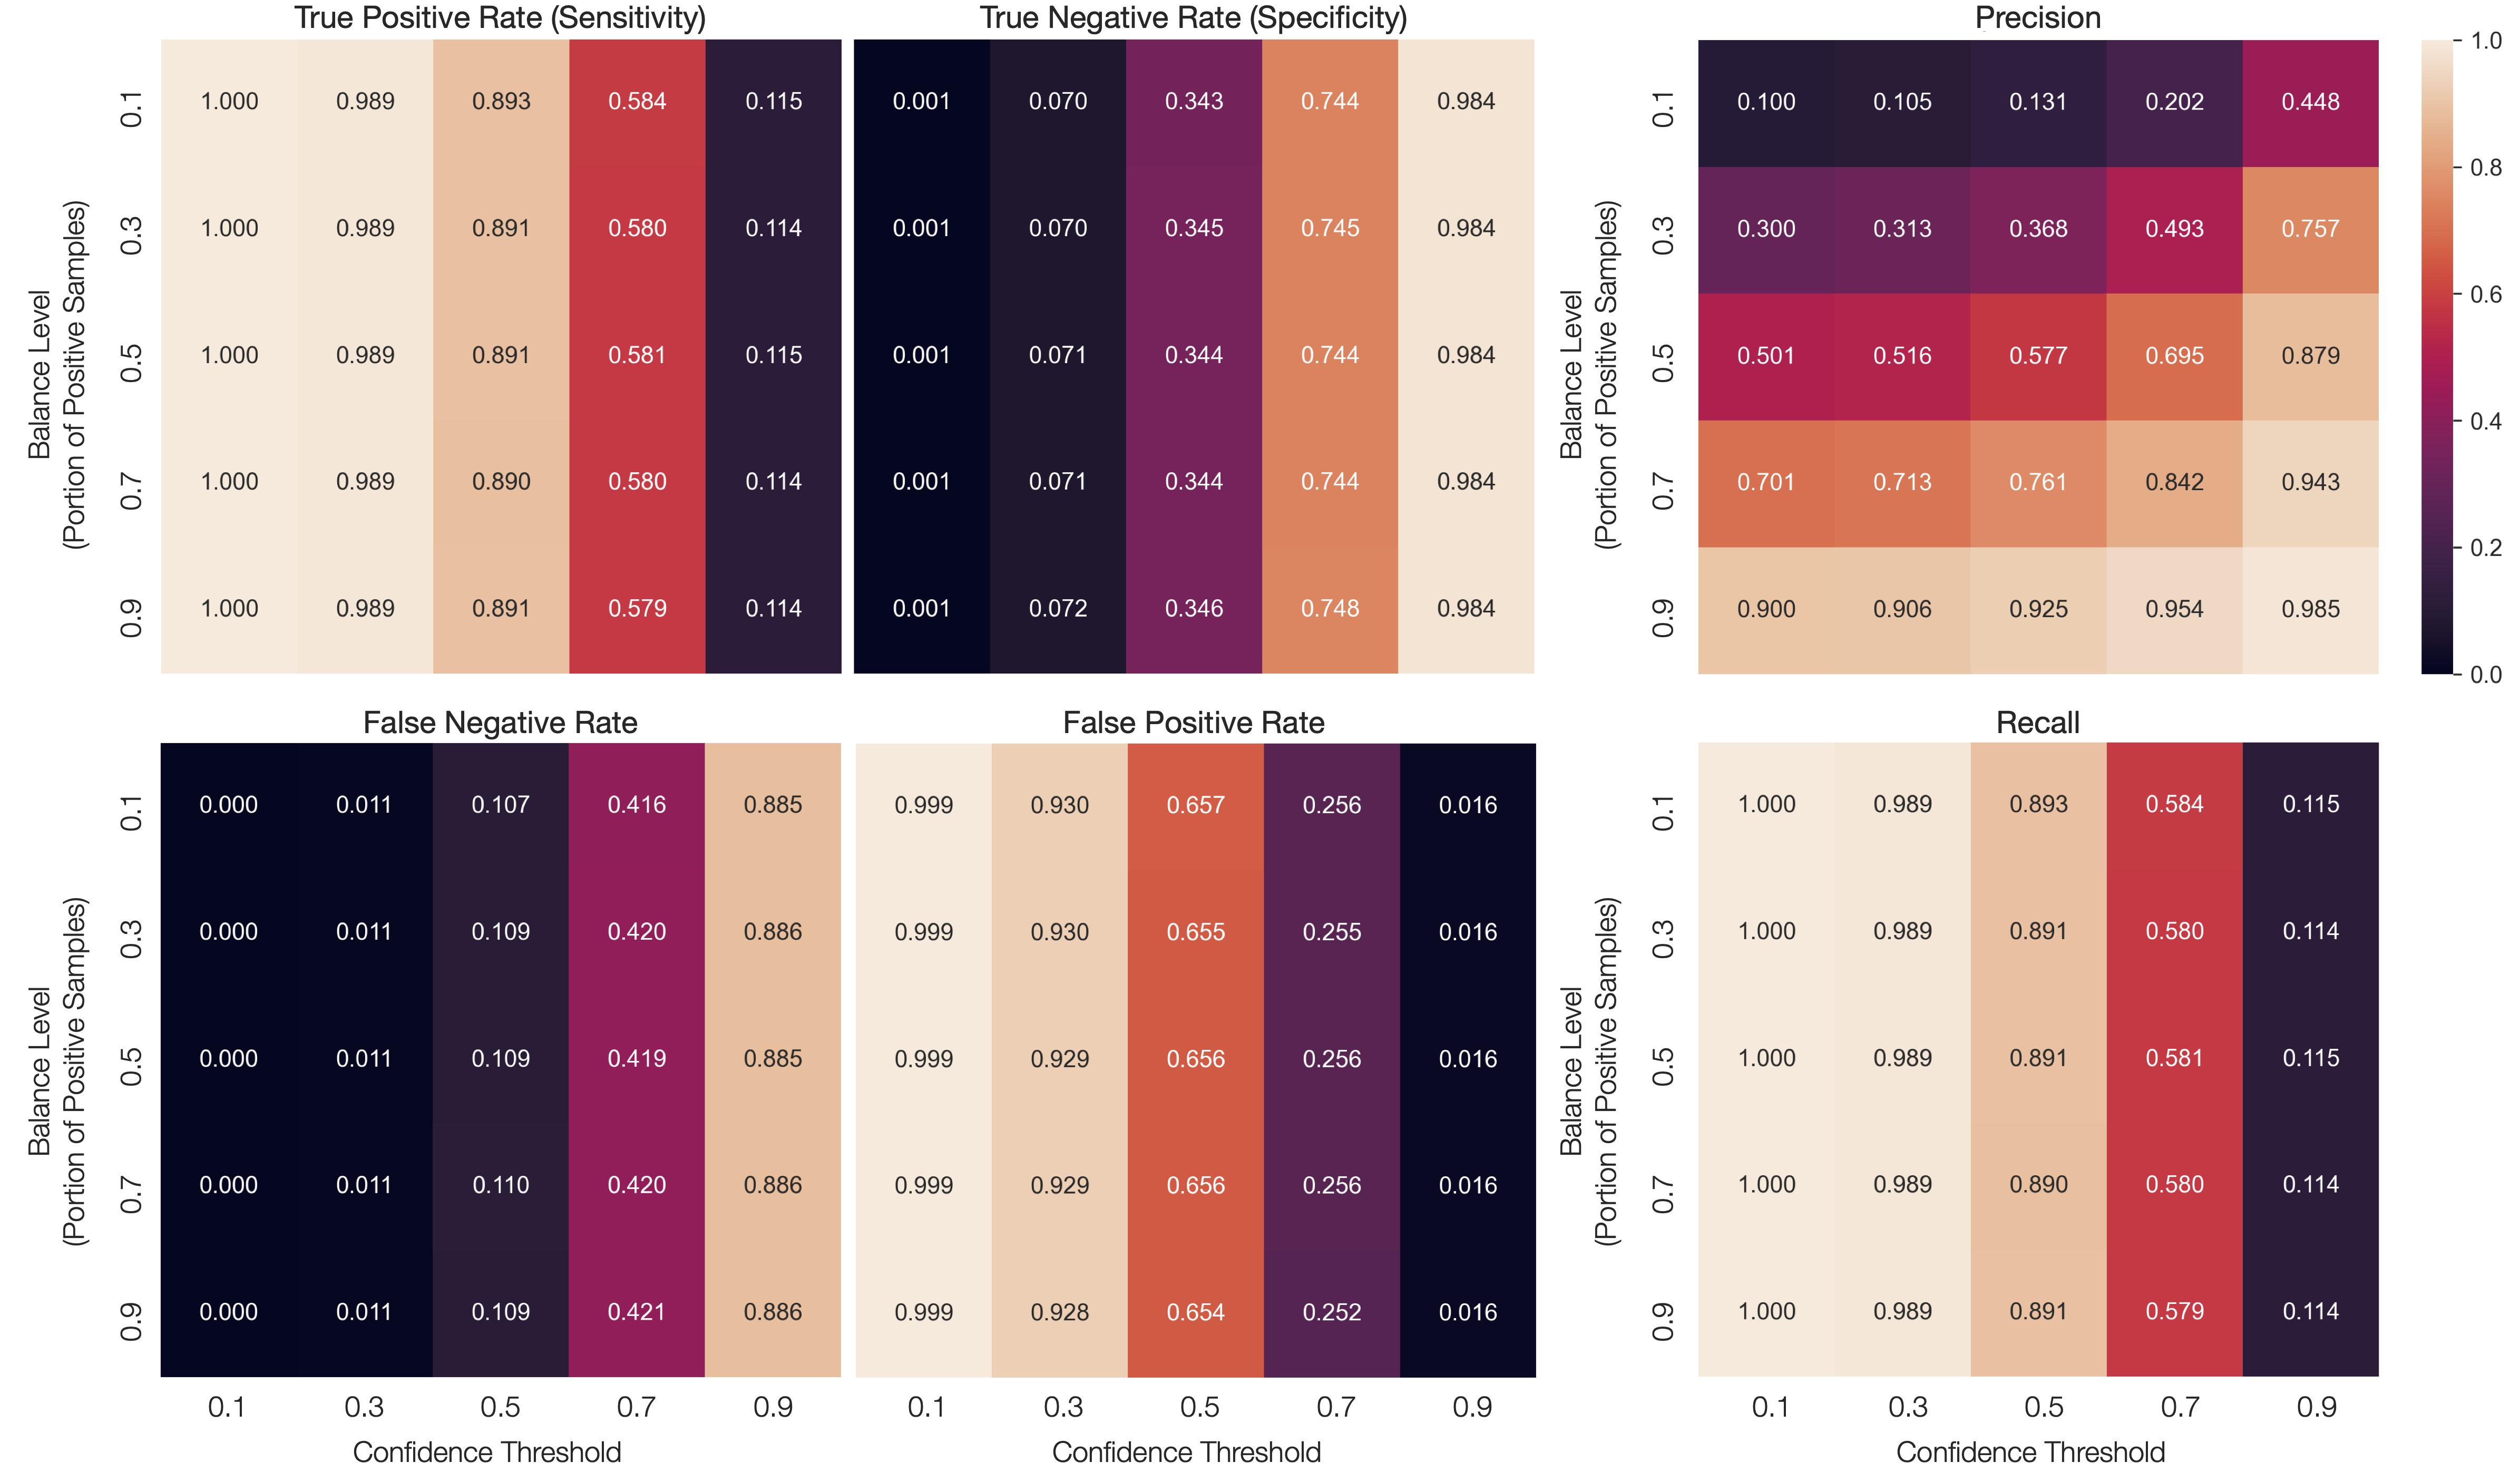
\includegraphics[width=1\textwidth]{fig_10.jpg}
    \caption{A 5 × 5 grid of performance metrics, with each cell representing a unique combination of balance and confidence threshold. The inspected metrics focus on one sample distribution at a time. The model is simulated to have higher false positive predictions than false negative predictions with a beta distribution of $\alpha=4$ and $\beta=3$ for the negative class.} 
    \label{fig:s5_1}
\end{figure}


Except for precision, metrics focused on a single sample distribution (i.e., actual positives or negatives) are unaffected by class imbalance (Figure~\ref{fig:s5_1}). For instance, the TPR remains stable at 0.989 with a confidence threshold of 0.3, regardless of the proportion of positive samples. This stability arises because such metrics evaluate only one distribution at a time, making them invariant to shifts in class balance.

To capture a more comprehensive view of model performance, multiple metrics are often combined. In this experiment, where false positives are more frequent than false negatives, TPR alone is insufficient, as it focuses only on actual positives. Including TNR accounts for false positives among actual negatives, revealing the model’s overall tendency to produce more false positives than false negatives. Since TNR and FPR (false positive rate) are complementary (TNR + FPR = 1), as are TPR and FNR (false negative rate), these pairs offer flexibility in reporting and interpreting classification errors. Researchers can choose to emphasize either the correctness (TPR and TNR) or error (FPR and FNR) aspects of model predictions, depending on the application context.

In agricultural disease diagnosis, both TPR (sensitivity) and TNR (specificity) are critical for evaluating performance. These metrics ensure accurate identification of both positive (diseased) and negative (healthy) cases. For example, Buczinski et al. (2018) used biometric indicators to detect bovine respiratory disease \citep{buczinski_validation_2018}, while Lu et al. (2017) relied on camera images to identify wheat stripe rust and black chaff \citep{lu_-field_2017}. These studies highlight the importance of sensitivity and specificity for balanced evaluations in diagnostic applications.

In contrast, precision and recall focus on predicted positive samples instead of actual positives, making them essential for tasks prioritizing prediction quality on positive samples over identifying all instances of interest. It is worth noting that precision measures the correctness of positive predictions and is highly sensitive to class imbalance and confidence thresholds. For example, in a dataset with 70\% positive samples, a naive model (i.e., when threshold = 0.1) predicting all samples as positive achieves a baseline precision of 0.7. It can only be considered modest improvement if a model reports a high precision of 0.8. However, in a dataset with only 10\% positive samples, achieving a precision of 0.448 with a high confidence threshold significantly outperforms the baseline of 0.1, demonstrating strong performance in handling imbalance even with a low value of precision in this case.

Compared to using the pair of TPR and TNR, precision and recall are particularly useful in computer vision domains like image-based weed detection \citep{zhang_automated_2019, su_advanced_2020}, where the goal is to identify weeds or economic crops, which may constitute rare positive samples, against a background of negative samples (e.g., areas with no objects of interest). In such cases, TNR and FPR are less relevant, as the focus is on the reliability of the model’s predictions (precision) and its ability to capture all positive instances of weeds or crops (recall). Similarly, in natural language processing (NLP) and information retrieval tasks \citep{gao_retrieval-augmented_2024, salemi_evaluating_2024}, precision and recall play vital roles. For example, in evaluating language models, the focus is often on how reliable the generated responses are (precision) and how many relevant responses are produced (recall). Negative samples, such as irrelevant or nonsensical outputs, are typically less of a concern compared to ensuring the relevance and completeness of positive samples. In information retrieval, where a user might submit a document containing ten key pieces of information (positive samples), the emphasis is on how many of these key pieces the system retrieves (recall) and how accurate those retrieved pieces are (precision), rather than on the proportion of irrelevant information correctly ignored (TNR).

In summary, each pair of metrics (TPR and TNR, precision and recall) offers a unique perspective on model performance. TPR (or sensitivity) and TNR (specificity) are essential for evaluating the model’s ability to correctly classify positive and negative samples, respectively, while precision and recall are indispensable metrics for scenarios where identifying and evaluating the quality of positive samples are more critical than focusing on the negative ones. These metrics are not self-explanatory but remain popular in the machine learning community due to their ability to measure the reliability and completeness of positive predictions in tasks where negative samples are of secondary interest.


\begin{figure}[H]
    \centering
    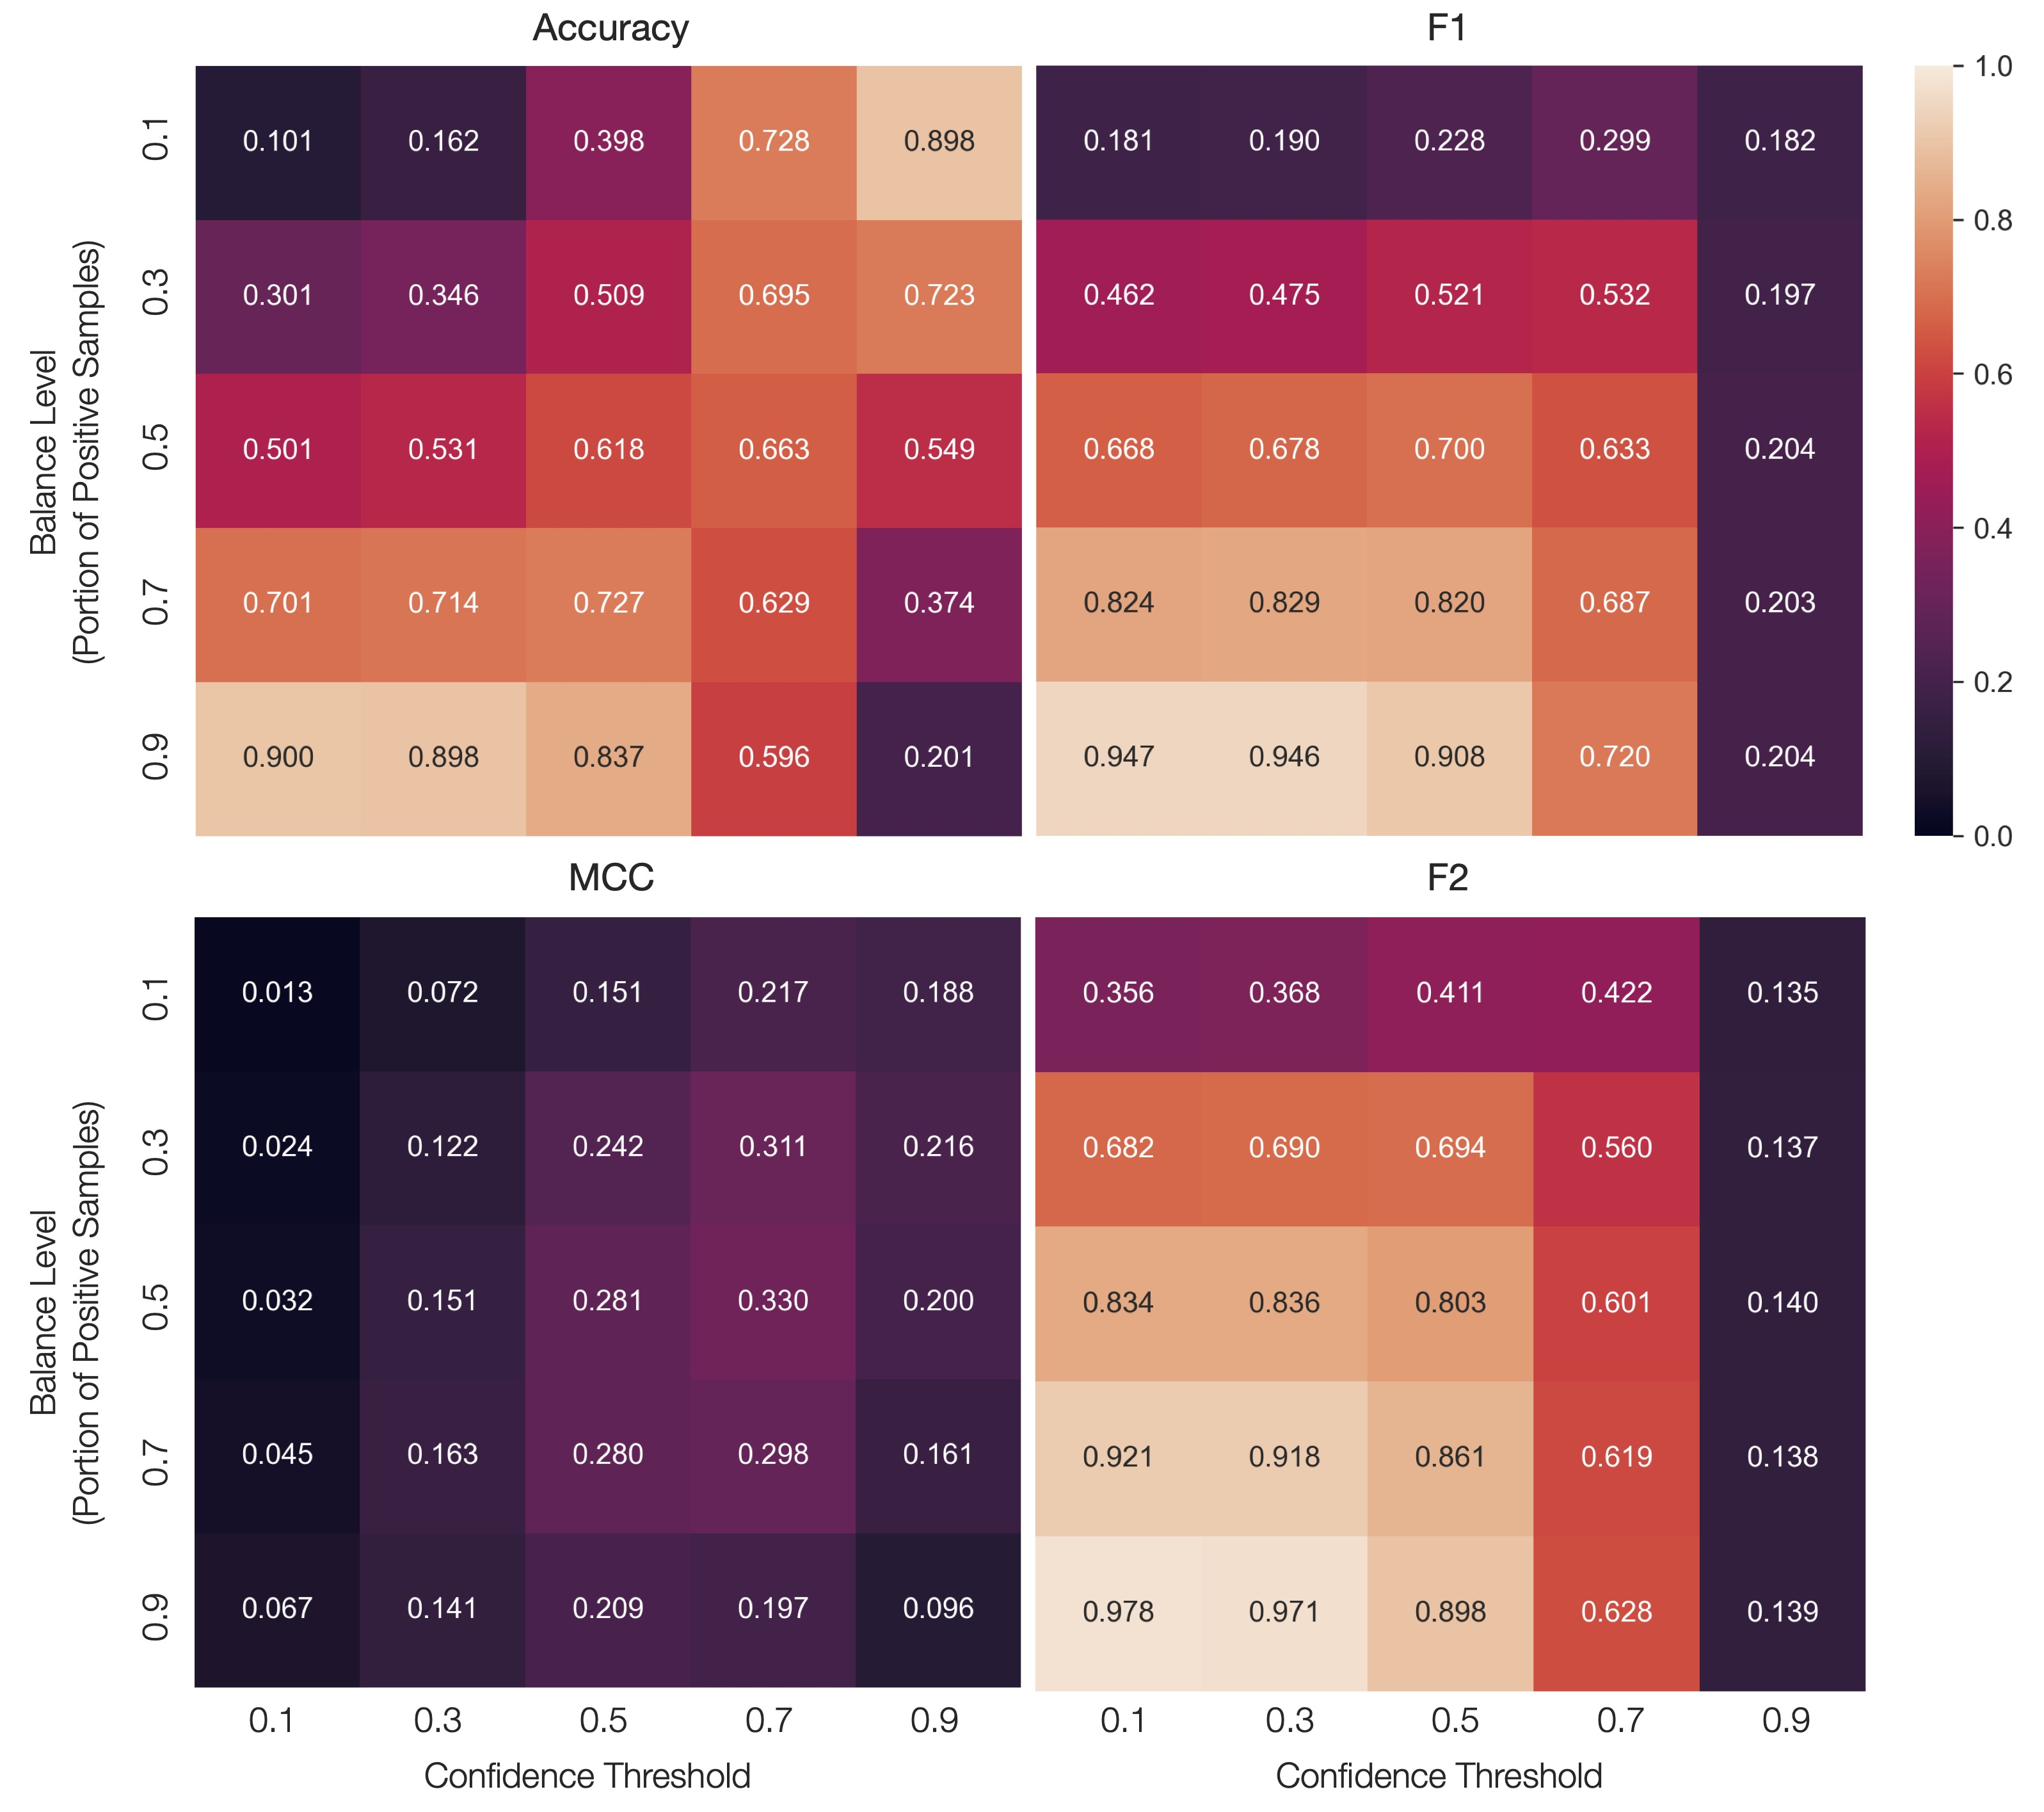
\includegraphics[width=.7\textwidth]{fig_11.jpg}
    \caption{A 5 × 5 grid of performance metrics, with each cell representing a unique combination of balance and confidence threshold. The inspected metrics focus on multiple sample distributions simultaneously. The prediction model is simulated to have higher false positive rate than false negative rate.}
    \label{fig:s5_2}
\end{figure}

Metrics that capture multiple aspects of model performance offer more comprehensive insights into a model’s effectiveness (Figure~\ref{fig:s5_2}). The heatmap in this experiment illustrates extreme scenarios at its corners, highlighting metric strengths and limitations. For example, the top-left corner features predominantly negative samples with mostly positive predictions, leading to many false positives, while the bottom-right corner features predominantly positive samples with mostly negative predictions, resulting in false negatives. The other corners illustrate cases where predictions align overwhelmingly with the majority class, allowing naive models to achieve high performance purely due to class imbalance rather than true predictive power. Effective metrics must assess performance beyond such “background effects.”

Accuracy, while simple and widely used, is limited in these extreme cases. For instance, in the top-left corner, accuracy drops due to false positives, whereas in corners dominated by a majority class, accuracy can be misleadingly high. For example, in the top-right corner, where 90\% of samples are negative, a model predicting all negatives achieves 90\% accuracy, despite ignoring true positives. Such scenarios demonstrate accuracy’s inability to capture critical trade-offs between false positives and false negatives.

The F1-score addresses accuracy’s limitations by balancing precision and TPR (i.e., recall), making it suitable for moderately imbalanced datasets. For example, in the same top-right corner of the heatmap, the F1-score of 0.182 reflects sensitivity to both false positives and false negatives, unlike accuracy, which may inflate performance due to imbalance. Real-world studies, such as Haque et al. (2023), underscore this: in a maize leaf blight detection task with a 1:2 class imbalance, an accuracy of 99.02\% masked the model’s limitations. Instead, an F1-score of 97.49\% provided a clearer measure of the model’s ability to balance precision and TPR \citep{haque_recognition_2023}.

Variants like the F2-score further refine performance evaluation by prioritizing TPR over precision, making it useful for scenarios where missing positive cases is costly. For instance, Minni (2024) applied the F2-score in breast cancer diagnosis to emphasize capturing positive cases, addressing the severe consequences of false negatives \citep{minni_exploring_2024}.

The MCC provides a robust alternative by considering all confusion matrix components and mitigating sensitivity to class imbalance. Becker et al. (2021) demonstrated MCC’s stability across datasets with varying imbalances, ranging from mildly (119 vs. 153 samples) to severely imbalanced (265 non-stress vs. 50 stress samples), when predicting heat stress in dairy cattle. Unlike F1-scores, which can reflect class distribution more than true classifier quality, MCC delivered a more comprehensive and reliable evaluation \citep{becker_predicting_2021}. These examples highlight MCC’s effectiveness in assessing model performance across diverse contexts.
\newpage

\section{Conclusion}

In summary, the review highlights several key considerations for performance assessment in predictive modeling. When evaluating regression models, the choice of metrics like Correlation Coefficient r, RMSE, and $R^2$ depends on the specific goals of the model. A comprehensive evaluation should include multiple metrics to understand different aspects of model performance. In binary classification models, precision and recall are crucial, but it is essential to correctly designate the positive class to avoid bias. Label-invariant metrics, such as the ROC curve and the proposed MCC curve, provide a balanced assessment, unaffected by class label choices.
Additionally, the reliability of model evaluation is significantly influenced by estimator choice and sample size. Larger sample sizes tend to reduce bias and variance, increasing evaluation reliability. Cross-validation methods, such as K-fold CV and LOOCV, are preferable for unbiased performance estimation, with the number of folds in K-fold CV being particularly influential in smaller datasets. Moreover, the review underscores the importance of correct implementation in model selection processes, as improper techniques can inflate performance estimates. This is especially true in complex models where feature selection and hyperparameter tuning need meticulous cross-validation to avoid overestimation of performance. Finally, the utility of Block CV is emphasized in contexts where block effects are significant. It provides a more realistic assessment of model generalizability and accuracy compared to a Random CV, which tends to overestimate performance in such scenarios.
Overall, the review recommends a thoughtful selection of metrics and evaluation techniques, tailored to the specific dataset and modeling objectives, to ensure accurate and reliable performance assessments in predictive modeling.

\section{Acknowledgement}
The author James Chen expresses his gratitude to Drs. Zhiwu Zhang, Hao Cheng, Gota Morota, and Gonzalo Ferreira for their insightful discussions that partially contributed to this study. The authors declare no conflicts of interest.

\newpage
%Bibliography
\bibliographystyle{unsrt}
\bibliography{references}

\newpage

\renewcommand{\theequation}{S.\arabic{equation}}
\renewcommand{\thefigure}{S.\arabic{figure}}
\renewcommand{\thetable}{S.\arabic{table}}

\section*{Appendix}

\subsection*{Cross Validation}

Model cross validation aims to evaluate how well a given model generalizes to an independent dataset that it has not seen during the training process. The most common method is K-fold cross-validation (\textbf{K-fold CV}). To implement the K-fold CV, the available dataset, denoted as $\mathcal{D}$, is partitioned into K equally sized folds. We can express the dataset as below:


\begin{equation} \label{eq_datasplit}
\begin{split}
    \mathcal{D} & = \{(X, Y)\} \\
    & = \{(X_1, Y_1), (X_2, Y_2), \dots, (X_K, Y_K)\}
\end{split}
\end{equation}

where $X\in\mathbb{R}^{n\times p}$ represents the input features, and $Y\in\mathbb{R}^{n\times1}$ symbolizes the ground truth labels for a single target variable. The value of n\ corresponds to the total number of samples, while p represents the number of features. In each iteration of the K-fold CV, a single fold is reserved as the test set, $\mathcal{D}_{\mathrm{test}}$ (or $\mathcal{D}_k$), to act as unseen data, while the remaining folds make up the training set $\mathcal{D}_{\mathrm{train}}$ (or $\mathcal{D}_\text{-k}$):

\begin{equation} \label{eq_traintest}
\begin{split}
    \mathcal{D}_{\text{train}} &= \mathcal{D}_{\text{-k}} \\
    &= \{(X_1, Y_1), (X_2, Y_2), \dots, (X_{k-1}, Y_{k-1}), (X_{k+1}, Y_{k+1}), \dots, (X_K, Y_K)\}\\
    \mathcal{D}_{\text{test}} &= \mathcal{D}_{k} \\
    &= \{(X_k, Y_k)\}
\end{split}
\end{equation}

After splitting the dataset into $\mathcal{D}_\text{-k}$ and $\mathcal{D}_k$, the examined model $f$ is trained on the training set $\mathcal{D}_\text{-k}$ and denoted as $f_{\mathcal{D}_{\text{-k}}}$. The hold-out test set $\mathcal{D}_k$ is then used to evaluate the model performance $\hat{g}\left(f_{\mathcal{D}_{\text{-k}}}\right)$, which is defined by comparing the predicted labels $\hat{Y}_{k} = f_{\mathcal{D}_{\text{-k}}}(X_k)$ with the true labels $Y_k$ using a performance metric $\mathcal{L}$ (e.g., RMSE or $R^2$):

\begin{equation} \label{eq_g_est}
    \begin{split}
\hat{g}(f_{\mathcal{D}_{\text{-k}}}) &= \mathcal{L}(Y_k, \hat{Y_k}) \\
    &= \mathcal{L}(Y_k, f_{\mathcal{D}_{\text{-k}}}(X_k))
    \end{split}
\end{equation}

To estimate the generalization performance of a model $\mathbb{E}[\hat{g}(f_\mathcal{D})]$, the K-fold CV procedure is repeated K times until each fold has been used as the test set $\mathcal{D}_k$ once. The entire dataset $\mathcal{D}$ is leveraged to calculate the average prediction performance over all K folds. The model's generalization performance can be expressed as:

\begin{equation} \label{eq_g_exp}
    \begin{split}
        \mathbb{E}[\hat{g}(f_{\mathcal{D}})] &= \mathbb{E}[\hat{g}(f_{\mathcal{D}_{\text{-k}}})] \\
        &= \frac{1}{K}\sum_{k=1}^{K} \hat{g}(f_{\mathcal{D}_{\text{-k}}})
    \end{split}
\end{equation}

It is noted that $\mathbb{E}[\hat{g}(f_\mathcal{D})]$ is equivalent to $\mathbb{E}[\hat{g}(f_{\mathcal{D}_{\text{-k}}})]$ in K-fold CV. It is because the $\mathbb{E}[\hat{g}(f_\mathcal{D})]$ is estimated by averaging all $\hat{g}(f_{\mathcal{D}_{\text{-k}}}) $ over K folds, which is also the definition of $\mathbb{E}[\hat{g}(f_{\mathcal{D}_{\text{-k}}})]$.

\subsection*{Cross Validation Bias and Variance}

The true generalization performance of the model $G(f_\mathcal{D})$ can only be approximated by averaging the performance metrics over infinite unseen datasets. However, in practice, the dataset $\mathcal{D}$ is finite and therefore, there is always a bias when using a finite dataset to estimate $G(f_\mathcal{D})$. The bias is known as validation bias:

\begin{equation} \label{eq_bias}
    \mathrm{Bias}=\mathbb{E}[\hat{g}\ (f_\mathcal{D})]-G(f_{D})
\end{equation}

For example, if RMSE is used as the performance metric, a positive validation bias suggests that the model validation procedure concludes a pessimistic estimation of the model performance, since the true performance is expected to be lower than the estimated performance.
Another aspect of model validation is the variance of the estimated performance. For example, in a 5-fold cross-validation, there are five estimates of the model performance. The variance among these five estimates is known as validation variance. A high validation variance suggests that the performance is sensitive to the choice of the test set $\mathcal{D}_k$, which may be caused by a small sample size or an over-complex model. The validation variance can be defined as:

\begin{equation} \label{eq_var}
    \begin{split}
        \mathrm{Variance}&=\mathbb{E}[(\hat{g}(f_{\mathcal{D}_{\text{-k}}})-\mathbb{E}[\hat{g}(f_\mathcal{D})])^{2}]\\
        &=\mathbb{E}[{\hat{g}}^2(f_{\mathcal{D}_{\text{-k}}}) - 2\hat{g}(f_{\mathcal{D}_{\text{-k}}})\mathbb{E}[\hat{g}(f_\mathcal{D})] + \mathbb{E}^{2}[\hat{g}(f_{\mathcal{D}})]]\\
        &=\mathbb{E}[{\hat{g}}^2(f_{\mathcal{D}_{\text{-k}}})] - 2\mathbb{E}[\hat{g}(f_{\mathcal{D}_{\text{-k}}})]\mathbb{E}[\hat{g}(f_{\mathcal{D}})] + \mathbb{E}^{2}[\hat{g}(f_{\mathcal{D}})]\\
        &=\mathbb{E}[{\hat{g}}^2(f_{\mathcal{D}_{\text{-k}}})] - \mathbb{E}^{2}[\hat{g}(f_{\mathcal{D}})]
    \end{split}
\end{equation}

Combining the Equations~\ref{eq_bias} and~\ref{eq_var}, the mean squared error (MSE) of the model validation can be decomposed as:

\begin{equation} \label{eq_tradeoff}
    \begin{split}
        \mathrm{MSE}&=\mathbb{E}[(\hat{g}(f_{\mathcal{D}_{\text{-k}}})-G(f_\mathcal{D}))^2]\\
        &=\mathbb{E}[{\hat{g}}^2(f_{\mathcal{D}_{\text{-k}}})] - 2\mathbb{E}[g(f_{D_\text{-k}})]G(f_\mathcal{D})+G^2(f_\mathcal{D}) +\\
        &\quad \; \mathbb{E}^2[\hat{g}(f_{\mathcal{D}_{\text{-k}}})] - \mathbb{E}^2[\hat{g}(f_{D_\text{-k}})]\\
        &=(\mathbb{E}^2[\hat{g}(f_{\mathcal{D}_{\text{-k}}})] - 2\mathbb{E}[\hat{g}(f_{D_\text{-k}})]G(f_{\mathcal{D}}) + G^{2}(f_{\mathcal{D}})) +\\
        &\quad \; (\mathbb{E}[{\hat{g}}^2(f_{\mathcal{D}_{\text{-k}}})]-\mathbb{E}^2[\hat{g}(f_{\mathcal{D}_{\text{-k}}})])\\
        &=(\mathbb{E}[\hat{g}(f_{\mathcal{D}_{\text{-k}}})]-G(f_{\mathcal{D}}))2+(\mathbb{E}[g2(f_{\mathcal{D}_{\text{-k}}})]-E^2[\hat{g}(f_{\mathcal{D}_{\text{-k}}})])\\
        &=(\mathbb{E}[\hat{g}(f_\mathcal{D})] - G(f_{\mathcal{D}}))^{2} +(\mathbb{E}[\hat{g}^2(f_{\mathcal{D}_{\text{-k}}})]-\mathbb{E}^2[\hat{g}(f_{\mathcal{D}})])\\
        &={\mathrm{Bias}}^2+\mathrm{Variance}
    \end{split}
\end{equation}

\subsection*{Hyperparameter}

Here are the loss functions for ordinary least squares (OLS), ridge regression, and LASSO regression, respectively:


\begin{equation} \label{eq_ols}
    \mathcal{L}_\text{OLS}(\beta)=\sum_{i=1}^{n}(y_i-x_i\beta)^2
\end{equation}

\begin{equation} \label{eq_ridge}
    \mathcal{L}_\text{ridge}(\beta)=\sum_{i=1}^{n}(y_i-x_i\beta)^2+\lambda\sum_{j=1}^{p}\beta_{j}^2
\end{equation}

\begin{equation} \label{eq_lasso}
    \mathcal{L}_\text{LASSO}(\beta)=\sum_{i=1}^{n}(y_i-x_i\beta)^2+\lambda\sum_{j=1}^{p}|\beta_j|
\end{equation}

Where $x_i$ and $y_i$ represent the ith row of the design matrix $X$ and the response vector Y, respectively. The term n denotes the sample size, and $\beta$ is the coefficient vector. All three models aim to find the optimal $\beta$ that minimizes their respective loss function, $\mathcal{L}$. In the regularized models (i.e., ridge and LASSO regression), the vector length of $\beta$ is penalized in the loss function.

\subsection*{Sqaured Correlation Coefficient $r^2$ and Determination Coefficient $R^2$}

The squared Pearson correlation coefficient, \( r^2 \), is not necessarily equivalent to the coefficient of determination, \( R^2 \). This equivalence holds true specifically in the context of least squares regression when the same model and data are used for both fitting and evaluation. However, this may not be the case when the model is assessed using new data. To demonstrate the equivalence between \( r^2 \) and \( R^2 \) under these specific conditions, we begin by assuming that the covariance between the predicted values \(\hat{Y}\) and the residuals \(\epsilon\) is zero:


\begin{equation} \label{eq_pf_cov}
    \begin{split}
        \text{cov}(Y, \hat{Y}) &= \text{cov}(\hat{Y} + \epsilon, \hat{Y}) \\
        &= \text{cov}(\hat{Y}, \hat{Y}) + \text{cov}(\hat{Y}, \epsilon) \\
        &= \text{var}(\hat{Y}) + \text{cov}(\hat{Y}, \epsilon) \\
        &= \text{var}(\hat{Y}) \\
    \end{split}
\end{equation}

With the assumption that \(\bar{\hat{Y}} = \bar{Y}\), which typically holds when \(\mathbb{E}[\epsilon] = 0\), the squared correlation coefficient \( r^2 \) is expressed as follows:

\begin{equation} \label{eq_pf_r2}
    \begin{split}
        r^2 &= \frac{\text{cov}^2(Y, \hat{Y})}{\text{var}(Y)\text{var}(\hat{Y})} \\
        &= \frac{\text{var}(\hat{Y})^2}{\text{var}(Y)\text{var}(\hat{Y})} \\
        &= \frac{\text{var}(\hat{Y})}{\text{var}(Y)} \\
        &= \frac{\sum\limits_{i=1}^{n}(\hat{Y}_i - \bar{\hat{Y}})^2}{\sum\limits_{i=1}^{n}(Y_i - \bar{Y})^2} \\
        &= \frac{\sum\limits_{i=1}^{n}(\hat{Y}_i - \bar{Y})^2}{\sum\limits_{i=1}^{n}(Y_i - \bar{Y})^2} \\
        &= \frac{SS_{\text{regression}}}{SS_{\text{total}}} \\
        &= R^2
    \end{split}
\end{equation}

where \(SS_{\text{regression}}\) is the variation explained by the model and \(SS_{\text{total}}\) is the total sum of squares. Each \(Y_i\) and \(\hat{Y}_i\) are the ith elements of the actual response vector \(Y\) and the predicted response vector \(\hat{Y}\), while \(\bar{Y}\) and \(\bar{\hat{Y}}\) are their respective means. This proof highlights that under certain assumptions, \( r^2 \) and \( R^2 \) can indeed be equivalent, but such conditions are specific to least squares regression where errors are normally distributed and predictions are unbiased estimates of the actual values.

\subsection*{Original results of the simulation experiments}

\begin{table}[ht!]
    \centering
    \caption{Experiment 2: ANOVA results of how each CV procedure affects the evaluation bias measured in the correlation coefficient (\textit{r}). FS: Feature Selection, HT: Hyperparameter Tuning. DF: Degree of Freedom, SS: Sum of Squares, MS: Mean Squares. Significant p-values (< 0.05) are highlighted in bold.}
    \label{tab:anova_r}
    \begin{minipage}{\textwidth}
    \subcaption{Dataset: Null dataset, Metric: \textit{r}}
    \centering
    \begin{tabular}{lcccccc}
    \toprule
    \textbf{Factor} & \textbf{DF} & \textbf{SS}    & \textbf{MS}    & \textbf{F-value}    & \textbf{p-value}  \\
    \midrule
    FS        & 1    & 49.72  & 49.72  & 20073.41   & \textbf{< 1e-6} \\
    HT        & 1    & 0.24   & 0.24   & 97.83      & \textbf{< 1e-6} \\
    FS:HT     & 1    & 0.03   & 0.03   & 14.33      & \textbf{< 1e-6} \\
    Residual  & 1996 & 4.94   & 0.00   & --         & --     \\
    \bottomrule
    \end{tabular}
    \end{minipage}
    \\[1em]
    \begin{minipage}{\textwidth}
    \subcaption{Dataset: Simulated spectral dataset, Metric: \textit{r}}
    \centering
    \begin{tabular}{lcccccc}
    \toprule
    \textbf{Factor} & \textbf{DF} & \textbf{SS}    & \textbf{MS}    & \textbf{F-value}    & \textbf{p-value}  \\
    \midrule
    FS        & 1    & 1.87e-03 & 1.87e-03 & 1.03  & 0.391  \\
    HT        & 1    & 1.64e-01 & 1.64e-01 & 91.10 & \textbf{< 1e-6}  \\
    FS:HT     & 1    & 2.85e-08 & 2.85e-08 & 0.00  & 0.997   \\
    Residual  & 1996 & 3.60e+00 & 1.80e-03 & --    & --      \\
    \bottomrule
    \end{tabular}
    \end{minipage}
    \\[1em]
    \begin{minipage}{\textwidth}
    \subcaption{Dataset: Real spectral dataset, Metric: \textit{r}}
    \centering
    \begin{tabular}{lcccccc}
    \toprule
    \textbf{Factor} & \textbf{DF} & \textbf{SS}    & \textbf{MS}    & \textbf{F-value}    & \textbf{p-value}  \\
    \midrule
    FS        & 1   & 2.31  & 2.31   & 1198.87 & \textbf{< 1e-6} \\
    HT        & 1   & 0.73  & 0.73   & 382.76  & \textbf{< 1e-6} \\
    FS:HT     & 1   & 0.00  & 0.00   & 0.20    & 0.648   \\
    Residual  & 1996 & 3.85  & 0.00   & --          & --              \\
    \bottomrule
    \end{tabular}
    \end{minipage}
\end{table}

\begin{table}[ht!]
    \centering
    \caption{Experiment 3: ANOVA results for the effect of deploying block CV and random CV. DF: Degree of Freedom, SS: Sum of Squares, MS: Mean Squares. Significant p-values (< 0.05) are highlighted in bold.}
    \label{tab:anova_all}
    % ---------------------------------------------------
    \begin{minipage}{\textwidth}
    \subcaption{Dataset: Simulated spectral dataset, Metric: \textit{r}}
    \centering
    \begin{tabular}{lcccccc}
    \toprule
    \textbf{Factor} & \textbf{DF} & \textbf{SS}    & \textbf{MS}    & \textbf{F-value}   & \textbf{p-value}      \\
    \midrule
    method    & 1    & 9.61    & 9.61   & 2122.69   & \textbf{< 1e-6} \\
    Residual  & 998 & 4.52    & 0.00   & --            & --            \\
    \bottomrule
    \end{tabular}
    \end{minipage}
    \\[1em]
    % ---------------------------------------------------
    \begin{minipage}{\textwidth}
    \subcaption{Dataset: Real spectral dataset, Metric: \textit{r}}
    \centering
    \begin{tabular}{lcccccc}
    \toprule
    \textbf{Factor} & \textbf{DF} & \textbf{SS}    & \textbf{MS}    & \textbf{F-value}   & \textbf{p-value}  \\
    \midrule
    method    & 1    & 8.64    & 8.64   & 29744.48  & \textbf{< 1e-6}          \\
    Residual  & 998  & 0.29    & 0.00   & --            & --           \\
    \bottomrule
    \end{tabular}
    \end{minipage}
    \\[1em]
    % ---------------------------------------------------
    \begin{minipage}{\textwidth}
    \subcaption{Dataset: Simulated spectral dataset, Metric: \textit{RMSE}}
    \centering
    \begin{tabular}{lcccccc}
    \toprule
    \textbf{Factor} & \textbf{DF} & \textbf{SS}     & \textbf{MS}     & \textbf{F-value}   & \textbf{p-value}     \\
    \midrule
    method    & 1    & 11.57   & 11.57   & 559.59     & \textbf{< 1e-6}  \\
    Residual  & 998  & 20.64   & 0.02    & --         & --            \\
    \bottomrule
    \end{tabular}
    \end{minipage}
    \\[1em]
    % ---------------------------------------------------
    \begin{minipage}{\textwidth}
    \subcaption{Dataset: Real spectral dataset, Metric: \textit{RMSE}}
    \centering
    \begin{tabular}{lcccccc}
    \toprule
    \textbf{Factor} & \textbf{DF} & \textbf{SS}    & \textbf{MS}    & \textbf{F-value}    & \textbf{p-value}  \\
    \midrule
    method    & 1    & 88.40   & 88.40   & 26768.87   & \textbf{< 1e-6}           \\
    Residual  & 998  & 3.29    & 0.00    & --         & --            \\
    \bottomrule
    \end{tabular}
    \end{minipage}
    % ---------------------------------------------------
\end{table}


\end{document}
